\documentclass[aspectratio=169,10pt]{beamer}
\usepackage{fontspec}
\setsansfont{TeX Gyre Heros}
\usepackage{booktabs}
\usepackage{pgfplots}
\usepackage{tikz}
\pgfplotsset{compat=1.18}
\usetikzlibrary{calc,positioning}

\definecolor{Navy}{HTML}{14213D}
\definecolor{Gold}{HTML}{D4A017}
\definecolor{Teal}{HTML}{2A9D8F}
\definecolor{Red}{HTML}{C94C4C}
\definecolor{Gray}{HTML}{6B7280}
\definecolor{LightGray}{HTML}{F5F6F8}
\definecolor{MidGray}{HTML}{D9DEE7}
\definecolor{PaleTeal}{HTML}{E8F5F2}
\definecolor{PaleRed}{HTML}{F9ECEC}
\definecolor{PaleGold}{HTML}{FBF4DF}

% Generated by presentation/build_presentation.py. Do not edit manually.
\newcommand{\GoogleRating}{4.5}
\newcommand{\TotalReviews}{298}
\newcommand{\CollectedAverage}{4.483}
\newcommand{\WrittenReviews}{220}
\newcommand{\WrittenCoverage}{73.8}
\newcommand{\PositiveRatingCount}{258}
\newcommand{\PositiveRatingPct}{86.6}
\newcommand{\NegativeRatingCount}{30}
\newcommand{\NegativeRatingPct}{10.1}
\newcommand{\RatingOneCount}{20}
\newcommand{\RatingOnePct}{6.7}
\newcommand{\RatingTwoCount}{10}
\newcommand{\RatingTwoPct}{3.4}
\newcommand{\RatingThreeCount}{10}
\newcommand{\RatingThreePct}{3.4}
\newcommand{\RatingFourCount}{24}
\newcommand{\RatingFourPct}{8.1}
\newcommand{\RatingFiveCount}{234}
\newcommand{\RatingFivePct}{78.5}
\newcommand{\RecentThirtyReviews}{14}
\newcommand{\RecentThirtyAverage}{3.93}
\newcommand{\PreviousThirtyReviews}{6}
\newcommand{\PreviousThirtyAverage}{3.67}
\newcommand{\RecentNinetyReviews}{28}
\newcommand{\RecentNinetyAverage}{3.68}
\newcommand{\PreviousNinetyReviews}{34}
\newcommand{\PreviousNinetyAverage}{3.91}
\newcommand{\HistoricalReviews}{270}
\newcommand{\HistoricalAverage}{4.57}
\newcommand{\RecentVsHistoricalDelta}{-0.89}
\newcommand{\RecentThirtyNegativePct}{28.6}
\newcommand{\PreviousThirtyNegativePct}{33.3}
\newcommand{\RecentThirtyNegativeDeltaAbs}{4.76}
\newcommand{\RecentThirtyDelta}{0.26}
\newcommand{\RecentNegativePct}{32.1}
\newcommand{\PreviousNinetyNegativePct}{20.6}
\newcommand{\RecentNinetyDelta}{-0.23}
\newcommand{\HistoricalNegativePct}{7.8}
\newcommand{\LatestReviewDate}{03 Sep 2026}
\newcommand{\EarliestReviewDate}{24 Dez 2024}
\newcommand{\RecentNinetyStart}{06 Jun 2026}
\newcommand{\RecentThirtyPerWeek}{3.27}
\newcommand{\RecentThirtyGap}{2.00}
\newcommand{\PreviousThirtyPerWeek}{1.40}
\newcommand{\PreviousThirtyGap}{3.81}
\newcommand{\CadenceFrequencyChange}{133.4}
\newcommand{\RecentThirtyStart}{05 Aug 2026}
\newcommand{\PreviousThirtyStart}{06 Jul 2026}
\newcommand{\RecentThirtyWritten}{11}
\newcommand{\PreviousThirtyWritten}{5}
\newcommand{\RecentThirtyFoodMentions}{9}
\newcommand{\RecentThirtyFoodCoverage}{81.8}
\newcommand{\RecentThirtyFoodPositive}{6}
\newcommand{\RecentThirtyFoodPositiveCoverage}{54.5}
\newcommand{\RecentThirtyFoodPositiveEvidence}{Mittel}
\newcommand{\RecentThirtyFoodNegative}{2}
\newcommand{\RecentThirtyFoodNegativeCoverage}{18.2}
\newcommand{\RecentThirtyFoodNegativeEvidence}{Niedrig}
\newcommand{\RecentThirtyFoodNeutral}{1}
\newcommand{\RecentThirtyServiceMentions}{10}
\newcommand{\RecentThirtyServiceCoverage}{90.9}
\newcommand{\RecentThirtyServicePositive}{7}
\newcommand{\RecentThirtyServicePositiveCoverage}{63.6}
\newcommand{\RecentThirtyServicePositiveEvidence}{Mittel}
\newcommand{\RecentThirtyServiceNegative}{1}
\newcommand{\RecentThirtyServiceNegativeCoverage}{9.1}
\newcommand{\RecentThirtyServiceNegativeEvidence}{Niedrig}
\newcommand{\RecentThirtyServiceNeutral}{2}
\newcommand{\RecentThirtyTasteMentions}{8}
\newcommand{\RecentThirtyTasteCoverage}{72.7}
\newcommand{\RecentThirtyTastePositive}{7}
\newcommand{\RecentThirtyTastePositiveCoverage}{63.6}
\newcommand{\RecentThirtyTastePositiveEvidence}{Mittel}
\newcommand{\RecentThirtyTasteNegative}{1}
\newcommand{\RecentThirtyTasteNegativeCoverage}{9.1}
\newcommand{\RecentThirtyTasteNegativeEvidence}{Niedrig}
\newcommand{\RecentThirtyTasteNeutral}{0}
\newcommand{\RecentThirtyDrinksMentions}{2}
\newcommand{\RecentThirtyDrinksCoverage}{18.2}
\newcommand{\RecentThirtyDrinksPositive}{0}
\newcommand{\RecentThirtyDrinksPositiveCoverage}{0.0}
\newcommand{\RecentThirtyDrinksPositiveEvidence}{Keine}
\newcommand{\RecentThirtyDrinksNegative}{1}
\newcommand{\RecentThirtyDrinksNegativeCoverage}{9.1}
\newcommand{\RecentThirtyDrinksNegativeEvidence}{Niedrig}
\newcommand{\RecentThirtyDrinksNeutral}{1}
\newcommand{\RecentThirtyBuffetMentions}{5}
\newcommand{\RecentThirtyBuffetCoverage}{45.5}
\newcommand{\RecentThirtyBuffetPositive}{3}
\newcommand{\RecentThirtyBuffetPositiveCoverage}{27.3}
\newcommand{\RecentThirtyBuffetPositiveEvidence}{Niedrig}
\newcommand{\RecentThirtyBuffetNegative}{1}
\newcommand{\RecentThirtyBuffetNegativeCoverage}{9.1}
\newcommand{\RecentThirtyBuffetNegativeEvidence}{Niedrig}
\newcommand{\RecentThirtyBuffetNeutral}{1}
\newcommand{\RecentThirtyMenuMentions}{2}
\newcommand{\RecentThirtyMenuCoverage}{18.2}
\newcommand{\RecentThirtyMenuPositive}{1}
\newcommand{\RecentThirtyMenuPositiveCoverage}{9.1}
\newcommand{\RecentThirtyMenuPositiveEvidence}{Niedrig}
\newcommand{\RecentThirtyMenuNegative}{1}
\newcommand{\RecentThirtyMenuNegativeCoverage}{9.1}
\newcommand{\RecentThirtyMenuNegativeEvidence}{Niedrig}
\newcommand{\RecentThirtyMenuNeutral}{0}
\newcommand{\RecentThirtyAtmosphereMentions}{5}
\newcommand{\RecentThirtyAtmosphereCoverage}{45.5}
\newcommand{\RecentThirtyAtmospherePositive}{5}
\newcommand{\RecentThirtyAtmospherePositiveCoverage}{45.5}
\newcommand{\RecentThirtyAtmospherePositiveEvidence}{Mittel}
\newcommand{\RecentThirtyAtmosphereNegative}{0}
\newcommand{\RecentThirtyAtmosphereNegativeCoverage}{0.0}
\newcommand{\RecentThirtyAtmosphereNegativeEvidence}{Keine}
\newcommand{\RecentThirtyAtmosphereNeutral}{0}
\newcommand{\RecentThirtyFriendlinessMentions}{2}
\newcommand{\RecentThirtyFriendlinessCoverage}{18.2}
\newcommand{\RecentThirtyFriendlinessPositive}{2}
\newcommand{\RecentThirtyFriendlinessPositiveCoverage}{18.2}
\newcommand{\RecentThirtyFriendlinessPositiveEvidence}{Niedrig}
\newcommand{\RecentThirtyFriendlinessNegative}{0}
\newcommand{\RecentThirtyFriendlinessNegativeCoverage}{0.0}
\newcommand{\RecentThirtyFriendlinessNegativeEvidence}{Keine}
\newcommand{\RecentThirtyFriendlinessNeutral}{0}
\newcommand{\RecentThirtyCommunicationMentions}{2}
\newcommand{\RecentThirtyCommunicationCoverage}{18.2}
\newcommand{\RecentThirtyCommunicationPositive}{0}
\newcommand{\RecentThirtyCommunicationPositiveCoverage}{0.0}
\newcommand{\RecentThirtyCommunicationPositiveEvidence}{Keine}
\newcommand{\RecentThirtyCommunicationNegative}{1}
\newcommand{\RecentThirtyCommunicationNegativeCoverage}{9.1}
\newcommand{\RecentThirtyCommunicationNegativeEvidence}{Niedrig}
\newcommand{\RecentThirtyCommunicationNeutral}{1}
\newcommand{\RecentThirtyParkingMentions}{1}
\newcommand{\RecentThirtyParkingCoverage}{9.1}
\newcommand{\RecentThirtyParkingPositive}{0}
\newcommand{\RecentThirtyParkingPositiveCoverage}{0.0}
\newcommand{\RecentThirtyParkingPositiveEvidence}{Keine}
\newcommand{\RecentThirtyParkingNegative}{1}
\newcommand{\RecentThirtyParkingNegativeCoverage}{9.1}
\newcommand{\RecentThirtyParkingNegativeEvidence}{Niedrig}
\newcommand{\RecentThirtyParkingNeutral}{0}
\newcommand{\PreviousThirtyFoodMentions}{4}
\newcommand{\PreviousThirtyFoodCoverage}{80.0}
\newcommand{\PreviousThirtyFoodPositive}{2}
\newcommand{\PreviousThirtyFoodPositiveCoverage}{40.0}
\newcommand{\PreviousThirtyFoodPositiveEvidence}{Niedrig}
\newcommand{\PreviousThirtyFoodNegative}{2}
\newcommand{\PreviousThirtyFoodNegativeCoverage}{40.0}
\newcommand{\PreviousThirtyFoodNegativeEvidence}{Niedrig}
\newcommand{\PreviousThirtyFoodNeutral}{0}
\newcommand{\PreviousThirtyServiceMentions}{4}
\newcommand{\PreviousThirtyServiceCoverage}{80.0}
\newcommand{\PreviousThirtyServicePositive}{2}
\newcommand{\PreviousThirtyServicePositiveCoverage}{40.0}
\newcommand{\PreviousThirtyServicePositiveEvidence}{Niedrig}
\newcommand{\PreviousThirtyServiceNegative}{2}
\newcommand{\PreviousThirtyServiceNegativeCoverage}{40.0}
\newcommand{\PreviousThirtyServiceNegativeEvidence}{Niedrig}
\newcommand{\PreviousThirtyServiceNeutral}{0}
\newcommand{\PreviousThirtyTasteMentions}{4}
\newcommand{\PreviousThirtyTasteCoverage}{80.0}
\newcommand{\PreviousThirtyTastePositive}{3}
\newcommand{\PreviousThirtyTastePositiveCoverage}{60.0}
\newcommand{\PreviousThirtyTastePositiveEvidence}{Niedrig}
\newcommand{\PreviousThirtyTasteNegative}{1}
\newcommand{\PreviousThirtyTasteNegativeCoverage}{20.0}
\newcommand{\PreviousThirtyTasteNegativeEvidence}{Niedrig}
\newcommand{\PreviousThirtyTasteNeutral}{0}
\newcommand{\PreviousThirtyDrinksMentions}{1}
\newcommand{\PreviousThirtyDrinksCoverage}{20.0}
\newcommand{\PreviousThirtyDrinksPositive}{0}
\newcommand{\PreviousThirtyDrinksPositiveCoverage}{0.0}
\newcommand{\PreviousThirtyDrinksPositiveEvidence}{Keine}
\newcommand{\PreviousThirtyDrinksNegative}{0}
\newcommand{\PreviousThirtyDrinksNegativeCoverage}{0.0}
\newcommand{\PreviousThirtyDrinksNegativeEvidence}{Keine}
\newcommand{\PreviousThirtyDrinksNeutral}{1}
\newcommand{\PreviousThirtyBuffetMentions}{1}
\newcommand{\PreviousThirtyBuffetCoverage}{20.0}
\newcommand{\PreviousThirtyBuffetPositive}{1}
\newcommand{\PreviousThirtyBuffetPositiveCoverage}{20.0}
\newcommand{\PreviousThirtyBuffetPositiveEvidence}{Niedrig}
\newcommand{\PreviousThirtyBuffetNegative}{0}
\newcommand{\PreviousThirtyBuffetNegativeCoverage}{0.0}
\newcommand{\PreviousThirtyBuffetNegativeEvidence}{Keine}
\newcommand{\PreviousThirtyBuffetNeutral}{0}
\newcommand{\PreviousThirtyMenuMentions}{0}
\newcommand{\PreviousThirtyMenuCoverage}{0.0}
\newcommand{\PreviousThirtyMenuPositive}{0}
\newcommand{\PreviousThirtyMenuPositiveCoverage}{0.0}
\newcommand{\PreviousThirtyMenuPositiveEvidence}{Keine}
\newcommand{\PreviousThirtyMenuNegative}{0}
\newcommand{\PreviousThirtyMenuNegativeCoverage}{0.0}
\newcommand{\PreviousThirtyMenuNegativeEvidence}{Keine}
\newcommand{\PreviousThirtyMenuNeutral}{0}
\newcommand{\PreviousThirtyAtmosphereMentions}{1}
\newcommand{\PreviousThirtyAtmosphereCoverage}{20.0}
\newcommand{\PreviousThirtyAtmospherePositive}{1}
\newcommand{\PreviousThirtyAtmospherePositiveCoverage}{20.0}
\newcommand{\PreviousThirtyAtmospherePositiveEvidence}{Niedrig}
\newcommand{\PreviousThirtyAtmosphereNegative}{0}
\newcommand{\PreviousThirtyAtmosphereNegativeCoverage}{0.0}
\newcommand{\PreviousThirtyAtmosphereNegativeEvidence}{Keine}
\newcommand{\PreviousThirtyAtmosphereNeutral}{0}
\newcommand{\PreviousThirtyFriendlinessMentions}{1}
\newcommand{\PreviousThirtyFriendlinessCoverage}{20.0}
\newcommand{\PreviousThirtyFriendlinessPositive}{1}
\newcommand{\PreviousThirtyFriendlinessPositiveCoverage}{20.0}
\newcommand{\PreviousThirtyFriendlinessPositiveEvidence}{Niedrig}
\newcommand{\PreviousThirtyFriendlinessNegative}{0}
\newcommand{\PreviousThirtyFriendlinessNegativeCoverage}{0.0}
\newcommand{\PreviousThirtyFriendlinessNegativeEvidence}{Keine}
\newcommand{\PreviousThirtyFriendlinessNeutral}{0}
\newcommand{\PreviousThirtyCommunicationMentions}{0}
\newcommand{\PreviousThirtyCommunicationCoverage}{0.0}
\newcommand{\PreviousThirtyCommunicationPositive}{0}
\newcommand{\PreviousThirtyCommunicationPositiveCoverage}{0.0}
\newcommand{\PreviousThirtyCommunicationPositiveEvidence}{Keine}
\newcommand{\PreviousThirtyCommunicationNegative}{0}
\newcommand{\PreviousThirtyCommunicationNegativeCoverage}{0.0}
\newcommand{\PreviousThirtyCommunicationNegativeEvidence}{Keine}
\newcommand{\PreviousThirtyCommunicationNeutral}{0}
\newcommand{\PreviousThirtyParkingMentions}{0}
\newcommand{\PreviousThirtyParkingCoverage}{0.0}
\newcommand{\PreviousThirtyParkingPositive}{0}
\newcommand{\PreviousThirtyParkingPositiveCoverage}{0.0}
\newcommand{\PreviousThirtyParkingPositiveEvidence}{Keine}
\newcommand{\PreviousThirtyParkingNegative}{0}
\newcommand{\PreviousThirtyParkingNegativeCoverage}{0.0}
\newcommand{\PreviousThirtyParkingNegativeEvidence}{Keine}
\newcommand{\PreviousThirtyParkingNeutral}{0}
\newcommand{\RecentTopPositiveOneName}{Service}
\newcommand{\RecentTopPositiveOneCount}{7}
\newcommand{\RecentTopPositiveOnePct}{63.6}
\newcommand{\RecentTopPositiveOneEvidence}{Mittel}
\newcommand{\RecentTopPositiveTwoName}{Geschmack}
\newcommand{\RecentTopPositiveTwoCount}{7}
\newcommand{\RecentTopPositiveTwoPct}{63.6}
\newcommand{\RecentTopPositiveTwoEvidence}{Mittel}
\newcommand{\RecentTopPositiveThreeName}{Speisen}
\newcommand{\RecentTopPositiveThreeCount}{6}
\newcommand{\RecentTopPositiveThreePct}{54.5}
\newcommand{\RecentTopPositiveThreeEvidence}{Mittel}
\newcommand{\RecentTopPositiveFourName}{Atmosphäre}
\newcommand{\RecentTopPositiveFourCount}{5}
\newcommand{\RecentTopPositiveFourPct}{45.5}
\newcommand{\RecentTopPositiveFourEvidence}{Mittel}
\newcommand{\RecentTopPositiveFiveName}{Buffet}
\newcommand{\RecentTopPositiveFiveCount}{3}
\newcommand{\RecentTopPositiveFivePct}{27.3}
\newcommand{\RecentTopPositiveFiveEvidence}{Niedrig}
\newcommand{\RecentTopPositiveSixName}{Komfort}
\newcommand{\RecentTopPositiveSixCount}{3}
\newcommand{\RecentTopPositiveSixPct}{27.3}
\newcommand{\RecentTopPositiveSixEvidence}{Niedrig}
\newcommand{\RecentTopNegativeOneName}{Speisen}
\newcommand{\RecentTopNegativeOneCount}{2}
\newcommand{\RecentTopNegativeOnePct}{18.2}
\newcommand{\RecentTopNegativeOneEvidence}{Niedrig}
\newcommand{\RecentTopNegativeTwoName}{Buffet}
\newcommand{\RecentTopNegativeTwoCount}{1}
\newcommand{\RecentTopNegativeTwoPct}{9.1}
\newcommand{\RecentTopNegativeTwoEvidence}{Niedrig}
\newcommand{\RecentTopNegativeThreeName}{Getränke}
\newcommand{\RecentTopNegativeThreeCount}{1}
\newcommand{\RecentTopNegativeThreePct}{9.1}
\newcommand{\RecentTopNegativeThreeEvidence}{Niedrig}
\newcommand{\RecentTopNegativeFourName}{Speisen Qualität}
\newcommand{\RecentTopNegativeFourCount}{1}
\newcommand{\RecentTopNegativeFourPct}{9.1}
\newcommand{\RecentTopNegativeFourEvidence}{Niedrig}
\newcommand{\RecentTopNegativeFiveName}{Speisenauswahl}
\newcommand{\RecentTopNegativeFiveCount}{1}
\newcommand{\RecentTopNegativeFivePct}{9.1}
\newcommand{\RecentTopNegativeFiveEvidence}{Niedrig}
\newcommand{\RecentTopNegativeSixName}{Frische}
\newcommand{\RecentTopNegativeSixCount}{1}
\newcommand{\RecentTopNegativeSixPct}{9.1}
\newcommand{\RecentTopNegativeSixEvidence}{Niedrig}
\newcommand{\OwnerOverallRate}{10.74}
\newcommand{\OwnerOverallResponses}{32}
\newcommand{\OwnerRecentThirtyRate}{0.0}
\newcommand{\OwnerPreviousThirtyRate}{0.0}
\newcommand{\OwnerRecentNinetyRate}{0.0}
\newcommand{\OwnerHistoricalRate}{11.85}
\newcommand{\LowScoreResponseRate}{3.33}
\newcommand{\LowScoreUnanswered}{29}
\newcommand{\RecentThirtyLowScores}{4}
\newcommand{\PreviousThirtyLowScores}{2}
\newcommand{\RecentThirtyLowScoreResponseRate}{0.0}
\newcommand{\PreviousThirtyLowScoreResponseRate}{0.0}
\newcommand{\OneStarResponseRate}{0.0}
\newcommand{\TwoStarResponseRate}{10.0}
\newcommand{\OwnerAverageDelay}{10.0}
\newcommand{\OwnerMedianDelay}{5.3}
\newcommand{\OneStarReviews}{20}
\newcommand{\OneStarShare}{6.71}
\newcommand{\OneStarWritten}{16}
\newcommand{\OneStarWrittenCoverage}{80.0}
\newcommand{\OneStarResponses}{0}
\newcommand{\TwoStarReviews}{10}
\newcommand{\TwoStarShare}{3.36}
\newcommand{\TwoStarWritten}{8}
\newcommand{\TwoStarWrittenCoverage}{80.0}
\newcommand{\TwoStarResponses}{1}
\newcommand{\LowScoreReviews}{30}
\newcommand{\LowScoreShare}{10.07}
\newcommand{\LowScoreWritten}{24}
\newcommand{\LowScoreWrittenCoverage}{80.0}
\newcommand{\LowScoreResponses}{1}
\newcommand{\HistoricalLowScores}{21}
\newcommand{\RecentLowScores}{9}
\newcommand{\LowServiceCount}{9}
\newcommand{\LowServicePct}{30.0}
\newcommand{\LowServiceEvidence}{Mittel}
\newcommand{\LowFoodCount}{10}
\newcommand{\LowFoodPct}{33.3}
\newcommand{\LowFoodEvidence}{Mittel}
\newcommand{\LowPriceCount}{5}
\newcommand{\LowPricePct}{16.7}
\newcommand{\LowPriceEvidence}{Mittel}
\newcommand{\LowTasteCount}{6}
\newcommand{\LowTastePct}{20.0}
\newcommand{\LowTasteEvidence}{Mittel}
\newcommand{\LowMenuCount}{1}
\newcommand{\LowMenuPct}{3.3}
\newcommand{\LowMenuEvidence}{Niedrig}
\newcommand{\LowDrinksCount}{1}
\newcommand{\LowDrinksPct}{3.3}
\newcommand{\LowDrinksEvidence}{Niedrig}
\newcommand{\LowBuffetCount}{1}
\newcommand{\LowBuffetPct}{3.3}
\newcommand{\LowBuffetEvidence}{Niedrig}
\newcommand{\LowRecentFoodHistorical}{5}
\newcommand{\LowRecentFoodRecent}{5}
\newcommand{\LowRecentFoodChange}{31.8}
\newcommand{\LowRecentTasteHistorical}{2}
\newcommand{\LowRecentTasteRecent}{4}
\newcommand{\LowRecentTasteChange}{34.9}
\newcommand{\LowRecentServiceHistorical}{6}
\newcommand{\LowRecentServiceRecent}{3}
\newcommand{\LowRecentServiceChange}{4.8}
\newcommand{\LowRecentPriceHistorical}{5}
\newcommand{\LowRecentPriceRecent}{0}
\newcommand{\LowRecentPriceChange}{-23.8}
\newcommand{\LowPairOneName}{Speisen + Speisen Qualität}
\newcommand{\LowPairOneCount}{6}
\newcommand{\LowPairOneShare}{20.0}
\newcommand{\LowPairTwoName}{Speisen + Geschmack}
\newcommand{\LowPairTwoCount}{5}
\newcommand{\LowPairTwoShare}{16.7}
\newcommand{\ServiceRating}{4.62}
\newcommand{\ServiceCoverage}{88.9}
\newcommand{\FoodRating}{4.57}
\newcommand{\FoodCoverage}{89.6}
\newcommand{\AtmosphereRating}{4.55}
\newcommand{\AtmosphereCoverage}{88.9}
\newcommand{\FoodTopicMentions}{165}
\newcommand{\FoodTopicPositive}{129}
\newcommand{\FoodTopicNegative}{11}
\newcommand{\FoodTopicNeutral}{25}
\newcommand{\FoodTopicNegativePct}{6.7}
\newcommand{\FoodTopicEvidence}{Hoch}
\newcommand{\FoodTopicNegativeEvidence}{Mittel}
\newcommand{\ServiceTopicMentions}{144}
\newcommand{\ServiceTopicPositive}{122}
\newcommand{\ServiceTopicNegative}{10}
\newcommand{\ServiceTopicNeutral}{12}
\newcommand{\ServiceTopicNegativePct}{6.9}
\newcommand{\ServiceTopicEvidence}{Hoch}
\newcommand{\ServiceTopicNegativeEvidence}{Mittel}
\newcommand{\TasteTopicMentions}{138}
\newcommand{\TasteTopicPositive}{125}
\newcommand{\TasteTopicNegative}{6}
\newcommand{\TasteTopicNeutral}{7}
\newcommand{\TasteTopicNegativePct}{4.3}
\newcommand{\TasteTopicEvidence}{Hoch}
\newcommand{\TasteTopicNegativeEvidence}{Mittel}
\newcommand{\FriendlinessTopicMentions}{58}
\newcommand{\FriendlinessTopicPositive}{56}
\newcommand{\FriendlinessTopicNegative}{2}
\newcommand{\FriendlinessTopicNeutral}{0}
\newcommand{\FriendlinessTopicNegativePct}{3.5}
\newcommand{\FriendlinessTopicEvidence}{Hoch}
\newcommand{\FriendlinessTopicNegativeEvidence}{Niedrig}
\newcommand{\AtmosphereTopicMentions}{54}
\newcommand{\AtmosphereTopicPositive}{43}
\newcommand{\AtmosphereTopicNegative}{0}
\newcommand{\AtmosphereTopicNeutral}{11}
\newcommand{\AtmosphereTopicNegativePct}{0.0}
\newcommand{\AtmosphereTopicEvidence}{Hoch}
\newcommand{\AtmosphereTopicNegativeEvidence}{Keine}
\newcommand{\PriceTopicMentions}{36}
\newcommand{\PriceTopicPositive}{20}
\newcommand{\PriceTopicNegative}{7}
\newcommand{\PriceTopicNeutral}{9}
\newcommand{\PriceTopicNegativePct}{19.4}
\newcommand{\PriceTopicEvidence}{Hoch}
\newcommand{\PriceTopicNegativeEvidence}{Mittel}
\newcommand{\BuffetTopicMentions}{29}
\newcommand{\BuffetTopicPositive}{18}
\newcommand{\BuffetTopicNegative}{3}
\newcommand{\BuffetTopicNeutral}{8}
\newcommand{\BuffetTopicNegativePct}{10.3}
\newcommand{\BuffetTopicEvidence}{Hoch}
\newcommand{\BuffetTopicNegativeEvidence}{Niedrig}
\newcommand{\AttentivenessTopicMentions}{23}
\newcommand{\AttentivenessTopicPositive}{21}
\newcommand{\AttentivenessTopicNegative}{2}
\newcommand{\AttentivenessTopicNeutral}{0}
\newcommand{\AttentivenessTopicNegativePct}{8.7}
\newcommand{\AttentivenessTopicEvidence}{Hoch}
\newcommand{\AttentivenessTopicNegativeEvidence}{Niedrig}
\newcommand{\CleanlinessTopicMentions}{19}
\newcommand{\CleanlinessTopicPositive}{16}
\newcommand{\CleanlinessTopicNegative}{0}
\newcommand{\CleanlinessTopicNeutral}{3}
\newcommand{\CleanlinessTopicNegativePct}{0.0}
\newcommand{\CleanlinessTopicEvidence}{Hoch}
\newcommand{\CleanlinessTopicNegativeEvidence}{Keine}
\newcommand{\PresentationTopicMentions}{18}
\newcommand{\PresentationTopicPositive}{13}
\newcommand{\PresentationTopicNegative}{0}
\newcommand{\PresentationTopicNeutral}{5}
\newcommand{\PresentationTopicNegativePct}{0.0}
\newcommand{\PresentationTopicEvidence}{Hoch}
\newcommand{\PresentationTopicNegativeEvidence}{Keine}
\newcommand{\FreshnessTopicMentions}{17}
\newcommand{\FreshnessTopicPositive}{13}
\newcommand{\FreshnessTopicNegative}{3}
\newcommand{\FreshnessTopicNeutral}{1}
\newcommand{\FreshnessTopicNegativePct}{17.6}
\newcommand{\FreshnessTopicEvidence}{Hoch}
\newcommand{\FreshnessTopicNegativeEvidence}{Niedrig}
\newcommand{\FoodQualityTopicMentions}{17}
\newcommand{\FoodQualityTopicPositive}{4}
\newcommand{\FoodQualityTopicNegative}{7}
\newcommand{\FoodQualityTopicNeutral}{6}
\newcommand{\FoodQualityTopicNegativePct}{41.2}
\newcommand{\FoodQualityTopicEvidence}{Hoch}
\newcommand{\FoodQualityTopicNegativeEvidence}{Mittel}
\newcommand{\TemperatureTopicMentions}{5}
\newcommand{\TemperatureTopicPositive}{1}
\newcommand{\TemperatureTopicNegative}{1}
\newcommand{\TemperatureTopicNeutral}{3}
\newcommand{\TemperatureTopicNegativePct}{20.0}
\newcommand{\TemperatureTopicEvidence}{Mittel}
\newcommand{\TemperatureTopicNegativeEvidence}{Niedrig}
\newcommand{\PortionTopicMentions}{5}
\newcommand{\PortionTopicPositive}{3}
\newcommand{\PortionTopicNegative}{0}
\newcommand{\PortionTopicNeutral}{2}
\newcommand{\PortionTopicNegativePct}{0.0}
\newcommand{\PortionTopicEvidence}{Mittel}
\newcommand{\PortionTopicNegativeEvidence}{Keine}
\newcommand{\DrinksTopicMentions}{7}
\newcommand{\DrinksTopicPositive}{3}
\newcommand{\DrinksTopicNegative}{2}
\newcommand{\DrinksTopicNeutral}{2}
\newcommand{\DrinksTopicNegativePct}{28.6}
\newcommand{\DrinksTopicEvidence}{Mittel}
\newcommand{\DrinksTopicNegativeEvidence}{Niedrig}
\newcommand{\WaitingTopicMentions}{5}
\newcommand{\WaitingTopicPositive}{0}
\newcommand{\WaitingTopicNegative}{4}
\newcommand{\WaitingTopicNeutral}{1}
\newcommand{\WaitingTopicNegativePct}{80.0}
\newcommand{\WaitingTopicEvidence}{Mittel}
\newcommand{\WaitingTopicNegativeEvidence}{Niedrig}
\newcommand{\MenuTopicMentions}{5}
\newcommand{\MenuTopicPositive}{2}
\newcommand{\MenuTopicNegative}{1}
\newcommand{\MenuTopicNeutral}{2}
\newcommand{\MenuTopicNegativePct}{20.0}
\newcommand{\MenuTopicEvidence}{Mittel}
\newcommand{\MenuTopicNegativeEvidence}{Niedrig}
\newcommand{\ParkingTopicMentions}{5}
\newcommand{\ParkingTopicPositive}{0}
\newcommand{\ParkingTopicNegative}{2}
\newcommand{\ParkingTopicNeutral}{3}
\newcommand{\ParkingTopicNegativePct}{40.0}
\newcommand{\ParkingTopicEvidence}{Mittel}
\newcommand{\ParkingTopicNegativeEvidence}{Niedrig}
\newcommand{\RecentLowRatingReviews}{9}
\newcommand{\RecentLowFood}{5}
\newcommand{\RecentLowService}{3}
\newcommand{\RecentLowTaste}{4}
\newcommand{\RecentLowMenu}{1}
\newcommand{\RecentLowParking}{1}
\newcommand{\ServicePeriodHistoricalMentions}{127}
\newcommand{\ServicePeriodHistoricalCoverage}{63.8}
\newcommand{\ServicePeriodHistoricalPositive}{110}
\newcommand{\ServicePeriodHistoricalNegative}{7}
\newcommand{\ServicePeriodHistoricalNeutral}{10}
\newcommand{\ServicePeriodHistoricalNegativeShare}{5.5}
\newcommand{\ServicePeriodHistoricalEvidence}{Hoch}
\newcommand{\ServicePeriodHistoricalNegativeEvidence}{Mittel}
\newcommand{\ServicePeriodRecentMentions}{17}
\newcommand{\ServicePeriodRecentCoverage}{81.0}
\newcommand{\ServicePeriodRecentPositive}{12}
\newcommand{\ServicePeriodRecentNegative}{3}
\newcommand{\ServicePeriodRecentNeutral}{2}
\newcommand{\ServicePeriodRecentNegativeShare}{17.6}
\newcommand{\ServicePeriodRecentEvidence}{Hoch}
\newcommand{\ServicePeriodRecentNegativeEvidence}{Niedrig}
\newcommand{\FoodPeriodHistoricalMentions}{148}
\newcommand{\FoodPeriodHistoricalCoverage}{74.4}
\newcommand{\FoodPeriodHistoricalPositive}{119}
\newcommand{\FoodPeriodHistoricalNegative}{6}
\newcommand{\FoodPeriodHistoricalNeutral}{23}
\newcommand{\FoodPeriodHistoricalNegativeShare}{4.0}
\newcommand{\FoodPeriodHistoricalEvidence}{Hoch}
\newcommand{\FoodPeriodHistoricalNegativeEvidence}{Mittel}
\newcommand{\FoodPeriodRecentMentions}{17}
\newcommand{\FoodPeriodRecentCoverage}{81.0}
\newcommand{\FoodPeriodRecentPositive}{10}
\newcommand{\FoodPeriodRecentNegative}{5}
\newcommand{\FoodPeriodRecentNeutral}{2}
\newcommand{\FoodPeriodRecentNegativeShare}{29.4}
\newcommand{\FoodPeriodRecentEvidence}{Hoch}
\newcommand{\FoodPeriodRecentNegativeEvidence}{Mittel}
\newcommand{\TastePeriodHistoricalMentions}{121}
\newcommand{\TastePeriodHistoricalCoverage}{60.8}
\newcommand{\TastePeriodHistoricalPositive}{112}
\newcommand{\TastePeriodHistoricalNegative}{2}
\newcommand{\TastePeriodHistoricalNeutral}{7}
\newcommand{\TastePeriodHistoricalNegativeShare}{1.6}
\newcommand{\TastePeriodHistoricalEvidence}{Hoch}
\newcommand{\TastePeriodHistoricalNegativeEvidence}{Niedrig}
\newcommand{\TastePeriodRecentMentions}{17}
\newcommand{\TastePeriodRecentCoverage}{81.0}
\newcommand{\TastePeriodRecentPositive}{13}
\newcommand{\TastePeriodRecentNegative}{4}
\newcommand{\TastePeriodRecentNeutral}{0}
\newcommand{\TastePeriodRecentNegativeShare}{23.5}
\newcommand{\TastePeriodRecentEvidence}{Hoch}
\newcommand{\TastePeriodRecentNegativeEvidence}{Niedrig}
\newcommand{\StrengthOneName}{Speisen}
\newcommand{\StrengthOneCount}{129}
\newcommand{\StrengthOneWidth}{3.80}
\newcommand{\StrengthTwoName}{Geschmack}
\newcommand{\StrengthTwoCount}{125}
\newcommand{\StrengthTwoWidth}{3.68}
\newcommand{\StrengthThreeName}{Service}
\newcommand{\StrengthThreeCount}{122}
\newcommand{\StrengthThreeWidth}{3.59}
\newcommand{\StrengthFourName}{Freundlichkeit des Personals}
\newcommand{\StrengthFourCount}{56}
\newcommand{\StrengthFourWidth}{1.65}
\newcommand{\StrengthFiveName}{Atmosphäre}
\newcommand{\StrengthFiveCount}{43}
\newcommand{\StrengthFiveWidth}{1.27}
\newcommand{\PriorityOneName}{Speisen}
\newcommand{\PriorityOneNegatives}{11}
\newcommand{\PriorityOneShare}{6.7}
\newcommand{\PriorityOneEvidence}{Mittel}
\newcommand{\PriorityOneRecent}{20.8}
\newcommand{\PriorityTwoName}{Speisen Qualität}
\newcommand{\PriorityTwoNegatives}{7}
\newcommand{\PriorityTwoShare}{41.2}
\newcommand{\PriorityTwoEvidence}{Mittel}
\newcommand{\PriorityTwoRecent}{12.3}
\newcommand{\PriorityThreeName}{Service}
\newcommand{\PriorityThreeNegatives}{10}
\newcommand{\PriorityThreeShare}{6.9}
\newcommand{\PriorityThreeEvidence}{Mittel}
\newcommand{\PriorityThreeRecent}{10.8}
\newcommand{\PriorityFourName}{Preis-Leistungs-Verhältnis}
\newcommand{\PriorityFourNegatives}{7}
\newcommand{\PriorityFourShare}{19.4}
\newcommand{\PriorityFourEvidence}{Mittel}
\newcommand{\PriorityFourRecent}{--}
\newcommand{\PriorityFiveName}{Wartezeit}
\newcommand{\PriorityFiveNegatives}{4}
\newcommand{\PriorityFiveShare}{80.0}
\newcommand{\PriorityFiveEvidence}{Niedrig}
\newcommand{\PriorityFiveRecent}{--}
\newcommand{\AtmosphereSignalReviews}{8}
\newcommand{\AtmosphereSignalChange}{20.5}
\newcommand{\AtmosphereSignalEvidence}{Mittel}
\newcommand{\FoodSignalReviews}{5}
\newcommand{\FoodSignalChange}{20.8}
\newcommand{\FoodSignalEvidence}{Mittel}
\newcommand{\ServiceSignalReviews}{3}
\newcommand{\ServiceSignalChange}{10.8}
\newcommand{\ServiceSignalEvidence}{Niedrig}
\newcommand{\TastePositiveRecent}{13}
\newcommand{\TastePositiveEvidence}{Mittel}
\newcommand{\TasteNegativeRecent}{4}
\newcommand{\TasteNegativeEvidence}{Niedrig}
\newcommand{\BuffetReviews}{29}
\newcommand{\BuffetCoverage}{13.2}
\newcommand{\BuffetPositiveCount}{18}
\newcommand{\BuffetPositivePct}{62.1}
\newcommand{\BuffetNegativeCount}{3}
\newcommand{\BuffetNegativePct}{10.3}
\newcommand{\BuffetNeutralCount}{8}
\newcommand{\BuffetNeutralPct}{27.6}
\newcommand{\BuffetQualityReviews}{1}
\newcommand{\BuffetVarietyReviews}{3}
\newcommand{\BuffetFreshnessReviews}{1}
\newcommand{\BuffetValueReviews}{3}
\newcommand{\BuffetReplenishmentReviews}{0}
\newcommand{\BuffetWaitingQueueReviews}{0}
\newcommand{\BuffetHistoricalMentions}{23}
\newcommand{\BuffetHistoricalCoverage}{11.6}
\newcommand{\BuffetHistoricalPositive}{14}
\newcommand{\BuffetHistoricalNegative}{2}
\newcommand{\BuffetHistoricalNeutral}{7}
\newcommand{\BuffetHistoricalAverage}{4.17}
\newcommand{\BuffetHistoricalEvidence}{Hoch}
\newcommand{\BuffetRecentMentions}{6}
\newcommand{\BuffetRecentCoverage}{28.6}
\newcommand{\BuffetRecentPositive}{4}
\newcommand{\BuffetRecentNegative}{1}
\newcommand{\BuffetRecentNeutral}{1}
\newcommand{\BuffetRecentAverage}{3.83}
\newcommand{\BuffetRecentEvidence}{Mittel}
\newcommand{\BuffetDays}{Saturday und Sunday}
\newcommand{\BuffetStart}{15:00}
\newcommand{\BuffetEnd}{20:00-21:00}
\newcommand{\DrinkMentions}{7}
\newcommand{\DrinkCoverage}{3.18}
\newcommand{\DrinkPositive}{3}
\newcommand{\DrinkNegative}{2}
\newcommand{\DrinkNeutral}{2}
\newcommand{\DrinkAverage}{3.29}
\newcommand{\DrinkEvidence}{Mittel}
\newcommand{\DrinkMenuItems}{34}
\newcommand{\DrinkItemsMentioned}{2}
\newcommand{\DrinkItemsUnmentioned}{32}
\newcommand{\DrinkMenuCoverage}{5.88}
\newcommand{\ColdDrinksItems}{15}
\newcommand{\ColdDrinksMentioned}{0}
\newcommand{\HotDrinksItems}{10}
\newcommand{\HotDrinksMentioned}{2}
\newcommand{\CocktailsItems}{9}
\newcommand{\CocktailsMentioned}{0}
\newcommand{\DrinkHistoricalMentions}{4}
\newcommand{\DrinkHistoricalCoverage}{2.0}
\newcommand{\DrinkHistoricalPositive}{3}
\newcommand{\DrinkHistoricalNegative}{1}
\newcommand{\DrinkHistoricalNeutral}{0}
\newcommand{\DrinkHistoricalAverage}{4.50}
\newcommand{\DrinkHistoricalEvidence}{Niedrig}
\newcommand{\DrinkRecentMentions}{3}
\newcommand{\DrinkRecentCoverage}{14.3}
\newcommand{\DrinkRecentPositive}{0}
\newcommand{\DrinkRecentNegative}{1}
\newcommand{\DrinkRecentNeutral}{2}
\newcommand{\DrinkRecentAverage}{1.67}
\newcommand{\DrinkRecentEvidence}{Niedrig}
\newcommand{\KitchenAttention}{337}
\newcommand{\KitchenPositive}{271}
\newcommand{\KitchenNegative}{27}
\newcommand{\KitchenNeutral}{39}
\newcommand{\KitchenMenuItems}{84}
\newcommand{\KitchenItemsMentioned}{14}
\newcommand{\KitchenMenuCoverage}{16.67}
\newcommand{\KitchenEvidence}{Hoch}
\newcommand{\BarAttention}{7}
\newcommand{\BarPositive}{3}
\newcommand{\BarNegative}{2}
\newcommand{\BarNeutral}{2}
\newcommand{\BarMenuItems}{34}
\newcommand{\BarItemsMentioned}{2}
\newcommand{\BarMenuCoverage}{5.88}
\newcommand{\BarEvidence}{Mittel}
\newcommand{\MenuItems}{118}
\newcommand{\MenuItemsMentioned}{16}
\newcommand{\MenuItemsUnmentioned}{102}
\newcommand{\MenuAttentionCoverage}{13.56}
\newcommand{\MenuCategoryOneName}{Salate}
\newcommand{\MenuCategoryOneMentions}{8}
\newcommand{\MenuCategoryOneItems}{4}
\newcommand{\MenuCategoryOneMentioned}{2}
\newcommand{\MenuCategoryTwoName}{Grillgerichte}
\newcommand{\MenuCategoryTwoMentions}{7}
\newcommand{\MenuCategoryTwoItems}{10}
\newcommand{\MenuCategoryTwoMentioned}{4}
\newcommand{\MenuCategoryThreeName}{Orientalische Gerichte}
\newcommand{\MenuCategoryThreeMentions}{6}
\newcommand{\MenuCategoryThreeItems}{8}
\newcommand{\MenuCategoryThreeMentioned}{1}
\newcommand{\MenuCategoryFourName}{Heißgetränke}
\newcommand{\MenuCategoryFourMentions}{4}
\newcommand{\MenuCategoryFourItems}{10}
\newcommand{\MenuCategoryFourMentioned}{2}
\newcommand{\MenuCategoryFiveName}{Kalte Vorspeisen}
\newcommand{\MenuCategoryFiveMentions}{3}
\newcommand{\MenuCategoryFiveItems}{11}
\newcommand{\MenuCategoryFiveMentioned}{3}
\newcommand{\MenuStatic}{true}
\newcommand{\FavouritesManual}{true}
\newcommand{\FavouritesNotUpdated}{true}
\newcommand{\WeeklyOffersAvailable}{false}
\newcommand{\BundlesAvailable}{false}
\newcommand{\DishRatingThreshold}{5}
\newcommand{\MansafMentions}{6}
\newcommand{\MansafReviewAverage}{5.0}
\newcommand{\MansafPositive}{2}
\newcommand{\MansafNegative}{0}
\newcommand{\MansafEvidence}{Mittel}
\newcommand{\TabboulehMentions}{5}
\newcommand{\TabboulehReviewAverage}{4.0}
\newcommand{\TabboulehPositive}{3}
\newcommand{\TabboulehNegative}{0}
\newcommand{\TabboulehEvidence}{Mittel}
\newcommand{\MixedGrillMentions}{4}
\newcommand{\MixedGrillReviewAverage}{2.5}
\newcommand{\MixedGrillPositive}{0}
\newcommand{\MixedGrillNegative}{2}
\newcommand{\MixedGrillEvidence}{Niedrig}
\newcommand{\DiscussedDishOneName}{Jordanisches Mansaf}
\newcommand{\DiscussedDishOneMentions}{6}
\newcommand{\DiscussedDishOnePositive}{2}
\newcommand{\DiscussedDishOneNegative}{0}
\newcommand{\DiscussedDishTwoName}{Tabbouleh}
\newcommand{\DiscussedDishTwoMentions}{5}
\newcommand{\DiscussedDishTwoPositive}{3}
\newcommand{\DiscussedDishTwoNegative}{0}
\newcommand{\DiscussedDishThreeName}{Gemischte Grillplatte}
\newcommand{\DiscussedDishThreeMentions}{4}
\newcommand{\DiscussedDishThreePositive}{0}
\newcommand{\DiscussedDishThreeNegative}{2}
\newcommand{\DiscussedDishFourName}{Tee}
\newcommand{\DiscussedDishFourMentions}{3}
\newcommand{\DiscussedDishFourPositive}{2}
\newcommand{\DiscussedDishFourNegative}{0}
\newcommand{\DiscussedDishFiveName}{Fattoush}
\newcommand{\DiscussedDishFiveMentions}{3}
\newcommand{\DiscussedDishFivePositive}{1}
\newcommand{\DiscussedDishFiveNegative}{0}
\newcommand{\EnglishWritten}{19}
\newcommand{\NonEnglishWritten}{201}
\newcommand{\TranslatedNonEnglish}{200}
\newcommand{\TranslationCoverage}{99.5}
\newcommand{\UsableTextReviews}{220}
\newcommand{\UsableTextCoverage}{73.8}
\newcommand{\DuplicateReviewIds}{0}
\newcommand{\InvalidReviews}{0}
\newcommand{\QuoteRecentFoodText}{Auch die übrigen Speisen waren abgestanden; einiges war trocken und bröselig.}
\newcommand{\QuoteRecentFoodMeta}{1 Stern | Aug 2026 | Aus dem Arabischen übersetzt\quad \href{https://www.google.com/maps/Bewertungen/data=!4m8!14m7!1m6!2m5!1sCi9DQUlRQUNvZENodHljRjlvT21Kc2VrbDZjRmQzWWpCWlJub3hjbXhqU1RoTE5IYxAB!2m1!1s0x0:0x27a031a79977995f!3m1!1s2@1:CAIQACodChtycF9oOmJsekl6cFd3YjBZRnoxcmxjSThLNHc\%7C\%7C?hl=en}{\color{Teal}\fontsize{6.1}{7.2}\selectfont\bfseries Originalbewertung öffnen $\rightarrow$}}
\newcommand{\QuoteRecentServiceText}{Die Servicekraft war überfordert und unfreundlich.}
\newcommand{\QuoteRecentServiceMeta}{1 Stern | Jul 2026 | Aus dem Deutschen übersetzt\quad \href{https://www.google.com/maps/Bewertungen/data=!4m8!14m7!1m6!2m5!1sCi9DQUlRQUNvZENodHljRjlvT2xodWRYUnJabmw1Vld0aFZGVmpNMVF6WlhjMFZVRRAB!2m1!1s0x0:0x27a031a79977995f!3m1!1s2@1:CAIQACodChtycF9oOlhudXRrZnl5VWthVFVjM1QzZXc0VUE\%7C\%7C?hl=en}{\color{Teal}\fontsize{6.1}{7.2}\selectfont\bfseries Originalbewertung öffnen $\rightarrow$}}
\newcommand{\QuoteRecentTasteText}{... es war zu trocken und schmeckte nicht gut.}
\newcommand{\QuoteRecentTasteMeta}{1 Stern | Jun 2026 | Aus dem Deutschen übersetzt\quad \href{https://www.google.com/maps/Bewertungen/data=!4m8!14m7!1m6!2m5!1sCi9DQUlRQUNvZENodHljRjlvT2pKUFJrZERaVXB2ZEZGeWJHbEtabk5GTFZkbk5VRRAB!2m1!1s0x0:0x27a031a79977995f!3m1!1s2@1:CAIQACodChtycF9oOjJPRkdDZUpvdFFybGlKZnNFLVdnNUE\%7C\%7C?hl=en}{\color{Teal}\fontsize{6.1}{7.2}\selectfont\bfseries Originalbewertung öffnen $\rightarrow$}}
\newcommand{\QuoteRecentMenuText}{Die Speisekarte wird auf einem Tablet angezeigt und ist dadurch äußerst unübersichtlich}
\newcommand{\QuoteRecentMenuMeta}{2 Sterne | Aug 2026 | Aus dem Deutschen übersetzt\quad \href{https://www.google.com/maps/Bewertungen/data=!4m8!14m7!1m6!2m5!1sChZDSUhNMG9nS0VKbnJfYUtMMi1yY1ZREAE!2m1!1s0x0:0x27a031a79977995f!3m1!1s2@1:CIHM0ogKEJnr\_aKL2-rcVQ\%7C\%7C?hl=en}{\color{Teal}\fontsize{6.1}{7.2}\selectfont\bfseries Originalbewertung öffnen $\rightarrow$}}
\newcommand{\QuoteStrengthFoodText}{Das Essen war köstlich und von hoher Qualität.}
\newcommand{\QuoteStrengthFoodMeta}{5 Sterne | Dez 2024 | Aus dem Deutschen übersetzt\quad \href{https://www.google.com/maps/Bewertungen/data=!4m8!14m7!1m6!2m5!1sChdDSUhNMG9nS0VJQ0FnSUNmOHZEbGxRRRAB!2m1!1s0x0:0x27a031a79977995f!3m1!1s2@1:CIHM0ogKEICAgICf8vDllQE\%7C\%7C?hl=en}{\color{Teal}\fontsize{6.1}{7.2}\selectfont\bfseries Originalbewertung öffnen $\rightarrow$}}
\newcommand{\QuoteStrengthServiceText}{Köstliches Essen, ein äußerst aufmerksamer und freundlicher Kellner ...}
\newcommand{\QuoteStrengthServiceMeta}{5 Sterne | Jun 2025 | Aus dem Deutschen übersetzt\quad \href{https://www.google.com/maps/Bewertungen/data=!4m8!14m7!1m6!2m5!1sCi9DQUlRQUNvZENodHljRjlvT2pjMlVtWjJiVEZwTTFJelNFWjBkME5JVkVoelVsRRAB!2m1!1s0x0:0x27a031a79977995f!3m1!1s2@1:CAIQACodChtycF9oOjc2UmZ2bTFpM1IzSEZ0d0NIVEhzUlE\%7C\%7C?hl=en}{\color{Teal}\fontsize{6.1}{7.2}\selectfont\bfseries Originalbewertung öffnen $\rightarrow$}}
\newcommand{\QuoteStrengthAtmosphereText}{Sowohl die Atmosphäre auf der Terrasse als auch das Ambiente innen waren sehr angenehm und gemütlich.}
\newcommand{\QuoteStrengthAtmosphereMeta}{5 Sterne | Aug 2026 | Aus dem Deutschen übersetzt\quad \href{https://www.google.com/maps/Bewertungen/data=!4m8!14m7!1m6!2m5!1sCi9DQUlRQUNvZENodHljRjlvT2tGUVIzQTVSbXhSWlV0VVpXOXRSWFppWlRVd1VIYxAB!2m1!1s0x0:0x27a031a79977995f!3m1!1s2@1:CAIQACodChtycF9oOkFQR3A5RmxRZUtUZW9tRXZiZTUwUHc\%7C\%7C?hl=en}{\color{Teal}\fontsize{6.1}{7.2}\selectfont\bfseries Originalbewertung öffnen $\rightarrow$}}
\newcommand{\QuoteServiceWaitText}{Der Service ist äußerst unfreundlich, und wir mussten sehr lange warten.}
\newcommand{\QuoteServiceWaitMeta}{2 Sterne | Mär 2026 | Aus dem Deutschen übersetzt\quad \href{https://www.google.com/maps/Bewertungen/data=!4m8!14m7!1m6!2m5!1sCi9DQUlRQUNvZENodHljRjlvT2xSWFUzVkhNMWRDV2pSVWVEVkNlSFUxVVZwWmRtYxAB!2m1!1s0x0:0x27a031a79977995f!3m1!1s2@1:CAIQACodChtycF9oOlRXU3VHM1dCWjRUeDVCeHU1UVpZdmc\%7C\%7C?hl=en}{\color{Teal}\fontsize{6.1}{7.2}\selectfont\bfseries Originalbewertung öffnen $\rightarrow$}}
\newcommand{\QuoteServiceUnresponsiveText}{Das Essen schmeckte furchtbar ... und das Personal reagierte nicht.}
\newcommand{\QuoteServiceUnresponsiveMeta}{1 Stern | Mai 2026\quad \href{https://www.google.com/maps/Bewertungen/data=!4m8!14m7!1m6!2m5!1sCi9DQUlRQUNvZENodHljRjlvT2pRd0xWbzNRMk5uUjJaVFMweEhkakZQUzBaamRsRRAB!2m1!1s0x0:0x27a031a79977995f!3m1!1s2@1:CAIQACodChtycF9oOjQwLVo3Q2NnR2ZTS0xHdjFPS0ZjdlE\%7C\%7C?hl=en}{\color{Teal}\fontsize{6.1}{7.2}\selectfont\bfseries Originalbewertung öffnen $\rightarrow$}}
\newcommand{\QuoteServiceOverwhelmedText}{Die Servicekraft war überfordert und unfreundlich.}
\newcommand{\QuoteServiceOverwhelmedMeta}{1 Stern | Jul 2026 | Aus dem Deutschen übersetzt\quad \href{https://www.google.com/maps/Bewertungen/data=!4m8!14m7!1m6!2m5!1sCi9DQUlRQUNvZENodHljRjlvT2xodWRYUnJabmw1Vld0aFZGVmpNMVF6WlhjMFZVRRAB!2m1!1s0x0:0x27a031a79977995f!3m1!1s2@1:CAIQACodChtycF9oOlhudXRrZnl5VWthVFVjM1QzZXc0VUE\%7C\%7C?hl=en}{\color{Teal}\fontsize{6.1}{7.2}\selectfont\bfseries Originalbewertung öffnen $\rightarrow$}}
\newcommand{\QuoteServicePositiveText}{Der Service ist ausgezeichnet, aufmerksam und freundlich.}
\newcommand{\QuoteServicePositiveMeta}{5 Sterne | Jan 2025 | Aus dem Deutschen übersetzt\quad \href{https://www.google.com/maps/Bewertungen/data=!4m8!14m7!1m6!2m5!1sChZDSUhNMG9nS0VJQ0FnSURfaC1lV1hnEAE!2m1!1s0x0:0x27a031a79977995f!3m1!1s2@1:CIHM0ogKEICAgID\_h-eWXg\%7C\%7C?hl=en}{\color{Teal}\fontsize{6.1}{7.2}\selectfont\bfseries Originalbewertung öffnen $\rightarrow$}}
\newcommand{\QuotePriceHighText}{Leider war es viel zu teuer.}
\newcommand{\QuotePriceHighMeta}{2 Sterne | Jan 2026 | Aus dem Deutschen übersetzt\quad \href{https://www.google.com/maps/Bewertungen/data=!4m8!14m7!1m6!2m5!1sCi9DQUlRQUNvZENodHljRjlvT21WdmFHSmZUR0YwTjBZMVJtcENlVzFHWkZOaVYwRRAB!2m1!1s0x0:0x27a031a79977995f!3m1!1s2@1:CAIQACodChtycF9oOmVvaGJfTGF0N0Y1RmpCeW1GZFNiV0E\%7C\%7C?hl=en}{\color{Teal}\fontsize{6.1}{7.2}\selectfont\bfseries Originalbewertung öffnen $\rightarrow$}}
\newcommand{\QuotePriceBuffetText}{Die Speisen am Buffet sind von schlechter Qualität, wodurch das Restaurant unnötig teuer wirkt.}
\newcommand{\QuotePriceBuffetMeta}{3 Sterne | Mär 2026 | Aus dem Deutschen übersetzt\quad \href{https://www.google.com/maps/Bewertungen/data=!4m8!14m7!1m6!2m5!1sCi9DQUlRQUNvZENodHljRjlvT20xeWFqY3piMVV4Ym1jeFRGRkVWbXhOU3kxNmEzYxAB!2m1!1s0x0:0x27a031a79977995f!3m1!1s2@1:CAIQACodChtycF9oOm1yajczb1UxbmcxTFFEVmxNSy16a3c\%7C\%7C?hl=en}{\color{Teal}\fontsize{6.1}{7.2}\selectfont\bfseries Originalbewertung öffnen $\rightarrow$}}
\newcommand{\QuotePricePositiveText}{15 € pro Person einschließlich Tee boten ein ausgezeichnetes Preis-Leistungs-Verhältnis.}
\newcommand{\QuotePricePositiveMeta}{5 Sterne | Dez 2025 | Aus dem Deutschen übersetzt\quad \href{https://www.google.com/maps/Bewertungen/data=!4m8!14m7!1m6!2m5!1sCi9DQUlRQUNvZENodHljRjlvT2xSRFQzaEJSa3N0Um1oUVdreFVlVGxHVEZONVRVRRAB!2m1!1s0x0:0x27a031a79977995f!3m1!1s2@1:CAIQACodChtycF9oOlRDT3hBRkstRmhQWkxUeTlGTFN5TUE\%7C\%7C?hl=en}{\color{Teal}\fontsize{6.1}{7.2}\selectfont\bfseries Originalbewertung öffnen $\rightarrow$}}
\newcommand{\QuoteFoodStaleText}{... leider waren die Speisen furchtbar und sehr abgestanden.}
\newcommand{\QuoteFoodStaleMeta}{1 Stern | Aug 2026 | Aus dem Arabischen übersetzt\quad \href{https://www.google.com/maps/Bewertungen/data=!4m8!14m7!1m6!2m5!1sCi9DQUlRQUNvZENodHljRjlvT21Kc2VrbDZjRmQzWWpCWlJub3hjbXhqU1RoTE5IYxAB!2m1!1s0x0:0x27a031a79977995f!3m1!1s2@1:CAIQACodChtycF9oOmJsekl6cFd3YjBZRnoxcmxjSThLNHc\%7C\%7C?hl=en}{\color{Teal}\fontsize{6.1}{7.2}\selectfont\bfseries Originalbewertung öffnen $\rightarrow$}}
\newcommand{\QuoteFoodUnappealingText}{... außerdem wurde kein Öl an den Tisch gebracht, und geschmacklich überzeugte das Essen keinen von uns vier.}
\newcommand{\QuoteFoodUnappealingMeta}{2 Sterne | Aug 2026 | Aus dem Deutschen übersetzt\quad \href{https://www.google.com/maps/Bewertungen/data=!4m8!14m7!1m6!2m5!1sChZDSUhNMG9nS0VKbnJfYUtMMi1yY1ZREAE!2m1!1s0x0:0x27a031a79977995f!3m1!1s2@1:CIHM0ogKEJnr\_aKL2-rcVQ\%7C\%7C?hl=en}{\color{Teal}\fontsize{6.1}{7.2}\selectfont\bfseries Originalbewertung öffnen $\rightarrow$}}
\newcommand{\QuoteFoodFreshText}{Das Essen war einfach ausgezeichnet - frisch zubereitet, aromatisch und schön angerichtet.}
\newcommand{\QuoteFoodFreshMeta}{5 Sterne | Aug 2026 | Aus dem Deutschen übersetzt\quad \href{https://www.google.com/maps/Bewertungen/data=!4m8!14m7!1m6!2m5!1sCi9DQUlRQUNvZENodHljRjlvT21sVU1HZHhPV3g0UVZaU2FGSXhkWGRJV0hONU0zYxAB!2m1!1s0x0:0x27a031a79977995f!3m1!1s2@1:CAIQACodChtycF9oOmlUMGdxOWx4QVZSaFIxdXdIWHN5M3c\%7C\%7C?hl=en}{\color{Teal}\fontsize{6.1}{7.2}\selectfont\bfseries Originalbewertung öffnen $\rightarrow$}}
\newcommand{\QuoteTasteDryText}{... es war zu trocken und schmeckte nicht gut.}
\newcommand{\QuoteTasteDryMeta}{1 Stern | Jun 2026 | Aus dem Deutschen übersetzt\quad \href{https://www.google.com/maps/Bewertungen/data=!4m8!14m7!1m6!2m5!1sCi9DQUlRQUNvZENodHljRjlvT2pKUFJrZERaVXB2ZEZGeWJHbEtabk5GTFZkbk5VRRAB!2m1!1s0x0:0x27a031a79977995f!3m1!1s2@1:CAIQACodChtycF9oOjJPRkdDZUpvdFFybGlKZnNFLVdnNUE\%7C\%7C?hl=en}{\color{Teal}\fontsize{6.1}{7.2}\selectfont\bfseries Originalbewertung öffnen $\rightarrow$}}
\newcommand{\QuoteTasteUnappealingText}{... außerdem wurde kein Öl an den Tisch gebracht, und geschmacklich überzeugte das Essen keinen von uns vier.}
\newcommand{\QuoteTasteUnappealingMeta}{2 Sterne | Aug 2026 | Aus dem Deutschen übersetzt\quad \href{https://www.google.com/maps/Bewertungen/data=!4m8!14m7!1m6!2m5!1sChZDSUhNMG9nS0VKbnJfYUtMMi1yY1ZREAE!2m1!1s0x0:0x27a031a79977995f!3m1!1s2@1:CIHM0ogKEJnr\_aKL2-rcVQ\%7C\%7C?hl=en}{\color{Teal}\fontsize{6.1}{7.2}\selectfont\bfseries Originalbewertung öffnen $\rightarrow$}}
\newcommand{\QuoteTastePositiveText}{Es ist köstlich und schmeckt hervorragend.}
\newcommand{\QuoteTastePositiveMeta}{5 Sterne | Jan 2025 | Aus dem Arabischen übersetzt\quad \href{https://www.google.com/maps/Bewertungen/data=!4m8!14m7!1m6!2m5!1sChdDSUhNMG9nS0VJQ0FnSUNmMjhMaDJBRRAB!2m1!1s0x0:0x27a031a79977995f!3m1!1s2@1:CIHM0ogKEICAgICf28Lh2AE\%7C\%7C?hl=en}{\color{Teal}\fontsize{6.1}{7.2}\selectfont\bfseries Originalbewertung öffnen $\rightarrow$}}
\newcommand{\QuoteAtmosphereRecentText}{Die Atmosphäre mit orientalischem Flair war großartig.}
\newcommand{\QuoteAtmosphereRecentMeta}{5 Sterne | Sep 2026\quad \href{https://www.google.com/maps/Bewertungen/data=!4m8!14m7!1m6!2m5!1sCi9DQUlRQUNvZENodHljRjlvT21GVlJVSmxNalpHV0hBNFdtaE5OV1ZoV0d4TVZrRRAB!2m1!1s0x0:0x27a031a79977995f!3m1!1s2@1:CAIQACodChtycF9oOmFVRUJlMjZGWHA4WmhNNWVhWGxMVkE\%7C\%7C?hl=en}{\color{Teal}\fontsize{6.1}{7.2}\selectfont\bfseries Originalbewertung öffnen $\rightarrow$}}
\newcommand{\QuoteBuffetPositiveText}{Mein Mann und ich waren heute zum zweiten Mal hier und haben das wunderbare Brunchbuffet genossen.}
\newcommand{\QuoteBuffetPositiveMeta}{5 Sterne | Sep 2025 | Aus dem Deutschen übersetzt\quad \href{https://www.google.com/maps/Bewertungen/data=!4m8!14m7!1m6!2m5!1sCi9DQUlRQUNvZENodHljRjlvT2pKM2JrcHliM1p1V1dOV2FreEtMV1JQZFVwTlRrRRAB!2m1!1s0x0:0x27a031a79977995f!3m1!1s2@1:CAIQACodChtycF9oOjJ3bkpyb3ZuWWNWakxKLWRPdUpNTkE\%7C\%7C?hl=en}{\color{Teal}\fontsize{6.1}{7.2}\selectfont\bfseries Originalbewertung öffnen $\rightarrow$}}
\newcommand{\QuoteBuffetNegativeText}{Die Speisen am Buffet sind von schlechter Qualität, wodurch das Restaurant unnötig teuer wirkt.}
\newcommand{\QuoteBuffetNegativeMeta}{3 Sterne | Mär 2026 | Aus dem Deutschen übersetzt\quad \href{https://www.google.com/maps/Bewertungen/data=!4m8!14m7!1m6!2m5!1sCi9DQUlRQUNvZENodHljRjlvT20xeWFqY3piMVV4Ym1jeFRGRkVWbXhOU3kxNmEzYxAB!2m1!1s0x0:0x27a031a79977995f!3m1!1s2@1:CAIQACodChtycF9oOm1yajczb1UxbmcxTFFEVmxNSy16a3c\%7C\%7C?hl=en}{\color{Teal}\fontsize{6.1}{7.2}\selectfont\bfseries Originalbewertung öffnen $\rightarrow$}}
\newcommand{\QuoteBuffetNeutralText}{Das Konzept wurde geändert, und es gab nur noch Buffet.}
\newcommand{\QuoteBuffetNeutralMeta}{3 Sterne | Jan 2026 | Aus dem Deutschen übersetzt\quad \href{https://www.google.com/maps/Bewertungen/data=!4m8!14m7!1m6!2m5!1sCi9DQUlRQUNvZENodHljRjlvT25jdE5WVmZTRk5OVm5sTE5HVmZiSEpaYVdKcWVWRRAB!2m1!1s0x0:0x27a031a79977995f!3m1!1s2@1:CAIQACodChtycF9oOnctNVVfSFNNVnlLNGVfbHJZaWJqeVE\%7C\%7C?hl=en}{\color{Teal}\fontsize{6.1}{7.2}\selectfont\bfseries Originalbewertung öffnen $\rightarrow$}}
\newcommand{\QuoteDrinkPositiveText}{Es gibt auch köstliche Getränke, zum Beispiel eine hervorragende Minzlimonade.}
\newcommand{\QuoteDrinkPositiveMeta}{5 Sterne | Nov 2025 | Aus dem Deutschen übersetzt\quad \href{https://www.google.com/maps/Bewertungen/data=!4m8!14m7!1m6!2m5!1sCi9DQUlRQUNvZENodHljRjlvT21saVowb3lNSFJHZWtKeFUwcEZYM1pWUVZCRFEyYxAB!2m1!1s0x0:0x27a031a79977995f!3m1!1s2@1:CAIQACodChtycF9oOmliZ0oyMHRGekJxU0pFX3ZVQVBDQ2c\%7C\%7C?hl=en}{\color{Teal}\fontsize{6.1}{7.2}\selectfont\bfseries Originalbewertung öffnen $\rightarrow$}}
\newcommand{\QuoteDrinkWrongText}{... wir erhielten das falsche Getränk.}
\newcommand{\QuoteDrinkWrongMeta}{2 Sterne | Aug 2026 | Aus dem Deutschen übersetzt\quad \href{https://www.google.com/maps/Bewertungen/data=!4m8!14m7!1m6!2m5!1sCi9DQUlRQUNvZENodHljRjlvT205UGNsZEdkbTlXUW10aVJUZGpjak5CY1hSQmFWRRAB!2m1!1s0x0:0x27a031a79977995f!3m1!1s2@1:CAIQACodChtycF9oOm9PcldGdm9WQmtiRTdjcjNBcXRBaVE\%7C\%7C?hl=en}{\color{Teal}\fontsize{6.1}{7.2}\selectfont\bfseries Originalbewertung öffnen $\rightarrow$}}
\newcommand{\QuoteDrinkPresentationText}{Außerdem wurden die Getränke früher in Gläsern mit Garnitur serviert,}
\newcommand{\QuoteDrinkPresentationMeta}{2 Sterne | Aug 2026 | Aus dem Deutschen übersetzt\quad \href{https://www.google.com/maps/Bewertungen/data=!4m8!14m7!1m6!2m5!1sChZDSUhNMG9nS0VKbnJfYUtMMi1yY1ZREAE!2m1!1s0x0:0x27a031a79977995f!3m1!1s2@1:CIHM0ogKEJnr\_aKL2-rcVQ\%7C\%7C?hl=en}{\color{Teal}\fontsize{6.1}{7.2}\selectfont\bfseries Originalbewertung öffnen $\rightarrow$}}
\newcommand{\QuoteDishMansafText}{Als Hauptgericht hatte ich jordanisches Mansaf, und es war köstlich.}
\newcommand{\QuoteDishMansafMeta}{5 Sterne | Feb 2025 | Aus dem Deutschen übersetzt\quad \href{https://www.google.com/maps/Bewertungen/data=!4m8!14m7!1m6!2m5!1sChZDSUhNMG9nS0VJQ0FnTURBaGR1VEZREAE!2m1!1s0x0:0x27a031a79977995f!3m1!1s2@1:CIHM0ogKEICAgMDAhduTFQ\%7C\%7C?hl=en}{\color{Teal}\fontsize{6.1}{7.2}\selectfont\bfseries Originalbewertung öffnen $\rightarrow$}}
\newcommand{\QuoteDishTabboulehText}{Tabbouleh und Fattoush waren ebenfalls sehr gut.}
\newcommand{\QuoteDishTabboulehMeta}{5 Sterne | Mai 2025 | Aus dem Deutschen übersetzt\quad \href{https://www.google.com/maps/Bewertungen/data=!4m8!14m7!1m6!2m5!1sChZDSUhNMG9nS0VJWFpoYmJGMWZieENBEAE!2m1!1s0x0:0x27a031a79977995f!3m1!1s2@1:CIHM0ogKEIXZhbbF1fbxCA\%7C\%7C?hl=en}{\color{Teal}\fontsize{6.1}{7.2}\selectfont\bfseries Originalbewertung öffnen $\rightarrow$}}
\newcommand{\QuoteDishMixedGrillText}{Die Hähnchenflügel auf der gemischten Grillplatte waren verbrannt.}
\newcommand{\QuoteDishMixedGrillMeta}{1 Stern | Jul 2026 | Aus dem Deutschen übersetzt\quad \href{https://www.google.com/maps/Bewertungen/data=!4m8!14m7!1m6!2m5!1sCi9DQUlRQUNvZENodHljRjlvT2xodWRYUnJabmw1Vld0aFZGVmpNMVF6WlhjMFZVRRAB!2m1!1s0x0:0x27a031a79977995f!3m1!1s2@1:CAIQACodChtycF9oOlhudXRrZnl5VWthVFVjM1QzZXc0VUE\%7C\%7C?hl=en}{\color{Teal}\fontsize{6.1}{7.2}\selectfont\bfseries Originalbewertung öffnen $\rightarrow$}}
\newcommand{\QuoteWaitingTimeText}{Der Service ist äußerst unfreundlich, und wir mussten sehr lange warten.}
\newcommand{\QuoteWaitingTimeMeta}{2 Sterne | Mär 2026 | Aus dem Deutschen übersetzt\quad \href{https://www.google.com/maps/Bewertungen/data=!4m8!14m7!1m6!2m5!1sCi9DQUlRQUNvZENodHljRjlvT2xSWFUzVkhNMWRDV2pSVWVEVkNlSFUxVVZwWmRtYxAB!2m1!1s0x0:0x27a031a79977995f!3m1!1s2@1:CAIQACodChtycF9oOlRXU3VHM1dCWjRUeDVCeHU1UVpZdmc\%7C\%7C?hl=en}{\color{Teal}\fontsize{6.1}{7.2}\selectfont\bfseries Originalbewertung öffnen $\rightarrow$}}
\newcommand{\QuoteMenuTabletText}{Die Speisekarte wird auf einem Tablet angezeigt und ist dadurch äußerst unübersichtlich}
\newcommand{\QuoteMenuTabletMeta}{2 Sterne | Aug 2026 | Aus dem Deutschen übersetzt\quad \href{https://www.google.com/maps/Bewertungen/data=!4m8!14m7!1m6!2m5!1sChZDSUhNMG9nS0VKbnJfYUtMMi1yY1ZREAE!2m1!1s0x0:0x27a031a79977995f!3m1!1s2@1:CIHM0ogKEJnr\_aKL2-rcVQ\%7C\%7C?hl=en}{\color{Teal}\fontsize{6.1}{7.2}\selectfont\bfseries Originalbewertung öffnen $\rightarrow$}}
\pgfplotsset{monthly axis ticks/.style={xtick={0,3,6,9,12,15,18,21},xticklabels={{Dez 24},{Mär 25},{Jun 25},{Sep 25},{Dez 25},{Mär 26},{Jun 26},{Sep 26}}}}

\hypersetup{colorlinks=false,pdfborder={0 0 0},pdfhighlight=/N}
\setbeamertemplate{navigation symbols}{}
\setbeamercolor{normal text}{fg=Navy,bg=white}
\setbeamercolor{frametitle}{fg=Navy,bg=white}
\setbeamerfont{frametitle}{series=\bfseries,size=\fontsize{18.5}{21.5}}
\setbeamertemplate{frametitle}{\vspace{0.08cm}\insertframetitle\par\vspace{0.02cm}\color{Gold}\rule{1.05cm}{1.8pt}\color{Navy}}
\setbeamersize{text margin left=0.66cm,text margin right=0.66cm}
\setbeamertemplate{footline}{\leavevmode\hbox{\begin{beamercolorbox}[wd=.78\paperwidth,ht=0.34cm,dp=0.13cm,leftskip=.66cm]{normal text}\color{Gray}\fontsize{6.2}{7.2}\selectfont Google-Bewertungsanalyse \enspace|\enspace Datenstand \LatestReviewDate\end{beamercolorbox}\begin{beamercolorbox}[wd=.22\paperwidth,ht=0.34cm,dp=0.13cm,rightskip=.66cm plus1fil]{normal text}\color{Gray}\fontsize{6.2}{7.2}\selectfont \insertframenumber/\inserttotalframenumber\end{beamercolorbox}}}
\setbeamertemplate{itemize item}{\color{Gold}\small\raise0.15ex\hbox{\textbullet}}
\setbeamertemplate{enumerate item}{\color{Navy}\bfseries\insertenumlabel.}

\newcommand{\sectiontag}[1]{{\color{Gold}\fontsize{6.8}{8}\selectfont\bfseries\MakeUppercase{#1}}\par\vspace{0.06cm}}
\newcommand{\smallcapslabel}[1]{{\color{Gray}\fontsize{7}{8.2}\selectfont\bfseries\MakeUppercase{#1}}}
\newcommand{\badge}[2]{\begingroup\setlength{\fboxsep}{0.07cm}\colorbox{#1}{\color{Navy}\fontsize{6.1}{7.2}\selectfont\bfseries #2}\endgroup}
\newcommand{\sourceReview}{\badge{PaleTeal}{KUNDEN-/DATENEVIDENZ}}
\newcommand{\sourceInternal}{\badge{PaleGold}{INTERNE BEOBACHTUNG}}
\newcommand{\sourceExperiment}{\badge{PaleRed}{VORGESCHLAGENES EXPERIMENT}}
\newcommand{\sourceData}{\badge{LightGray}{BENÖTIGTE DATEN}}
\newcommand{\pillbutton}[3]{\begingroup\setlength{\fboxsep}{0.10cm}\hyperlink{#1}{\colorbox{#3}{\color{white}\fontsize{6.8}{8}\selectfont\bfseries #2\ $\rightarrow$}}\endgroup}
\newcommand{\goldbutton}[2]{\pillbutton{#1}{#2}{Gold}}
\newcommand{\tealbutton}[2]{\pillbutton{#1}{#2}{Teal}}
\newcommand{\redbutton}[2]{\pillbutton{#1}{#2}{Red}}
\newcommand{\backbutton}[2]{\begingroup\setlength{\fboxsep}{0.10cm}\hyperlink{#1}{\colorbox{Navy}{\color{white}\fontsize{6.8}{8}\selectfont\bfseries $\leftarrow$\ #2}}\endgroup}
\newcommand{\quotebox}[3]{\begingroup\setlength{\fboxsep}{0.12cm}\colorbox{#1}{\parbox{\dimexpr\linewidth-0.24cm\relax}{\raggedright{\fontsize{7.1}{8.2}\selectfont\itshape ``#2''}\par\vspace{0.04cm}{\color{Gray}\fontsize{5.4}{6.2}\selectfont #3}}}\endgroup}
\newcommand{\quoteneg}[2]{\quotebox{PaleRed}{#1}{#2}}
\newcommand{\quotepos}[2]{\quotebox{PaleTeal}{#1}{#2}}
\newcommand{\quotegray}[2]{\quotebox{LightGray}{#1}{#2}}
\newcommand{\kpicard}[4]{\colorbox{#1}{\parbox[c][1.18cm][c]{0.92\linewidth}{\centering\smallcapslabel{#2}\par\vspace{0.04cm}{\color{#4}\fontsize{20}{22}\selectfont\bfseries #3}}}}
\newcommand{\countsentimentbar}[3]{\begin{tikzpicture}[x=0.058cm,y=1cm]\pgfmathsetmacro{\PosEnd}{#1/(#1+#2+#3)*100}\pgfmathsetmacro{\NeuEnd}{(#1+#2)/(#1+#2+#3)*100}\fill[Teal,rounded corners=1.2pt] (0,0) rectangle (\PosEnd,0.38);\fill[Gray!35] (\PosEnd,0) rectangle (\NeuEnd,0.38);\fill[Red] (\NeuEnd,0) rectangle (100,0.38);\end{tikzpicture}}
\newcommand{\implication}[1]{\colorbox{Navy}{\parbox{0.965\linewidth}{\color{white}\fontsize{7.6}{9}\selectfont\textbf{Managementfolgerung:} #1}}}
\newcommand{\evidenceitem}[3]{{\fontsize{7.7}{9.2}\selectfont\textbf{#1}\hfill #2\quad #3}\par\vspace{0.07cm}}
\newcommand{\appendixhead}[1]{\sectiontag{Evidenzanhang #1}\vspace{0.05cm}}
\newcommand{\casecard}[6]{\begingroup\setlength{\fboxsep}{0.09cm}\colorbox{LightGray}{\parbox[c][2.18cm][t]{0.975\linewidth}{\vspace{0.05cm}{\color{Navy}\fontsize{7}{8.1}\selectfont\bfseries #1\quad #2}\par\vspace{0.02cm}{\fontsize{6.35}{7.45}\selectfont #3}\par{\color{Gray}\fontsize{6.05}{7.15}\selectfont #4}\par{\fontsize{6.25}{7.35}\selectfont\itshape #5}\par\vfill\hfill #6}}\endgroup\par\vspace{0.08cm}}
\newcommand{\opcasecard}[6]{\begingroup\setlength{\fboxsep}{0.09cm}\colorbox{LightGray}{\parbox[c][2.49cm][t]{0.975\linewidth}{\vspace{0.05cm}{\color{Navy}\fontsize{7}{8.1}\selectfont\bfseries #1\quad #2}\par\vspace{0.02cm}{\fontsize{6.35}{7.45}\selectfont #3}\par{\color{Gray}\fontsize{6.05}{7.15}\selectfont #4}\par{\fontsize{6.25}{7.35}\selectfont\itshape #5}\par\vfill\hfill #6}}\endgroup\par\vspace{0.08cm}}
\newcommand{\dishcard}[4]{\begingroup\setlength{\fboxsep}{0.09cm}\colorbox{PaleTeal}{\parbox[c][1.54cm][t]{0.975\linewidth}{\vspace{0.04cm}{\color{Navy}\fontsize{7.2}{8.3}\selectfont\bfseries #1}\par{\fontsize{6.2}{7.3}\selectfont #2}\par{\fontsize{6.1}{7.2}\selectfont\itshape ``#3''}\hfill #4}}\endgroup\par\vspace{0.06cm}}
\newcommand{\chapterdivider}[7]{\begin{frame}[plain]\hypertarget{#6}{}\begin{tikzpicture}[remember picture,overlay]\fill[Navy] (current page.south west) rectangle (current page.north east);\fill[#7] (current page.south west) rectangle ([xshift=0.18cm]current page.north west);\end{tikzpicture}\vfill{\color{#7}\fontsize{10}{12}\selectfont\bfseries KAPITEL #1}\par\vspace{0.14cm}{\color{white}\fontsize{28}{32}\selectfont\bfseries #2}\par\vspace{0.34cm}\begin{columns}[T,onlytextwidth]\column{0.31\textwidth}{\color{white!55}\fontsize{6.5}{7.5}\selectfont\bfseries WAS DIE DATEN ZEIGEN}\par\vspace{0.05cm}{\color{white}\fontsize{8}{9.5}\selectfont #3}\column{0.31\textwidth}{\color{white!55}\fontsize{6.5}{7.5}\selectfont\bfseries WARUM DAS WICHTIG IST}\par\vspace{0.05cm}{\color{white}\fontsize{8}{9.5}\selectfont #4}\column{0.31\textwidth}{\color{white!55}\fontsize{6.5}{7.5}\selectfont\bfseries EMPFOHLENE MASSNAHME}\par\vspace{0.05cm}{\color{white}\fontsize{8}{9.5}\selectfont #5}\end{columns}\vfill\goldbutton{#6-content}{Kapitel öffnen}\end{frame}}

\begin{document}

\begin{frame}[plain]
  \hypertarget{m-cover}{}\begin{tikzpicture}[remember picture,overlay]\fill[Navy] (current page.south west) rectangle (current page.north east);\fill[Gold] (current page.south west) rectangle ([xshift=0.20cm]current page.north west);\fill[Gold,opacity=.17] ([xshift=-4.3cm,yshift=-1.0cm]current page.north east) circle (3.1cm);\fill[Teal,opacity=.14] ([xshift=-1.1cm,yshift=1.0cm]current page.south east) circle (2.15cm);\end{tikzpicture}
  \vspace{0.85cm}{\color{Gold}\fontsize{9.5}{11.5}\selectfont\bfseries MANAGEMENTANALYSE}\par\vspace{0.38cm}{\color{white}\fontsize{34}{38}\selectfont\bfseries Al Assiel Restaurant\\[-0.02cm]\& Shisha}\par\vspace{0.25cm}{\color{white!82}\fontsize{14}{18}\selectfont Managementüberblick, operative Evidenz und klare Verantwortlichkeiten}\par\vfill{\color{white}\fontsize{10}{12}\selectfont Bonn, Deutschland}\par\vspace{0.08cm}{\color{white!68}\fontsize{8.4}{10}\selectfont \TotalReviews\ Google Bewertungen | \WrittenReviews\ Bewertungen mit Text | Datenstand \LatestReviewDate}\vspace{0.44cm}
\end{frame}

\begin{frame}{Präsentationsübersicht}
  \hypertarget{m-roadmap}{}\sectiontag{So nutzen Sie diese Präsentation}
  \begin{columns}[T,onlytextwidth]
    \column{0.48\textwidth}{\fontsize{7.2}{8.6}\selectfont\textbf{1 Managementüberblick}\quad Kernaussage und Priorität\par\textbf{2 Entwicklung im letzten Monat}\quad Letzte gegenüber vorherigen 30 Tagen\par\textbf{3 Leistungstrends}\quad Monats- und 90-Tage-Kontext\par\textbf{4 Bewertungsfluss \& Antwort}\quad Frequenz und Nachverfolgung\par\textbf{5 Bad Bewertungen}\quad Muster und 30 operative Fälle\par\textbf{6 Service}\quad Evidenz wiederkehrender Schwächen\par\textbf{7 Küche / Speisen / Geschmack}\quad Stärke plus aktuelle Prüfungen\par\textbf{8 Bar \& Getränke}\quad Aufmerksamkeits- und Erlebnissignale}
    \column{0.48\textwidth}{\fontsize{7.2}{8.6}\selectfont\textbf{9 Buffet}\quad Sentiment und Monitoringbedarf\par\textbf{10 Speisekarte \& Bestellung}\quad Grenzen der Bewertungen und POS-Bedarf\par\textbf{11 Erwähnte Gerichte}\quad Alle beobachteten Artikel\par\textbf{12 Managementbeobachtungen}\quad Nach Herkunft getrennte Eingaben\par\textbf{13 Aktionsplan}\quad Sofortige gegenüber evidenzabhängiger Arbeit\par\textbf{14 Delegation}\quad Vier verantwortliche Arbeitsbereiche\par\textbf{15 KPI-Steuerung}\quad Wöchentliches Steuerungsdashboard\par\textbf{16 Evidenzanhang}\quad Fallregister, Links und Checklisten}
  \end{columns}
  \vfill\goldbutton{m-ch1}{Kapitel 1 starten}\quad\tealbutton{m-ch16}{Evidenzanhang öffnen}
\end{frame}

\chapterdivider{1}{Managementüberblick}{Der langfristige Ruf ist stark, aber die jüngste Gästeerfahrung und Nachbearbeitung sind schwächer.}{Das Management sollte die Marke schützen und zugleich auf aktuelle operative Signale reagieren.}{Managementprioritäten setzen und Detailbelege gezielt öffnen.}{m-ch1}{Gold}

\begin{frame}{Starker Ruf; die jüngste Entwicklung braucht weiterhin Aufmerksamkeit}
  \hypertarget{m-ch1-content}{}\hypertarget{m-exec}{}\sectiontag{Kapitel 1 - Managementüberblick}
  \begin{columns}[T,onlytextwidth]\column{0.235\textwidth}\kpicard{PaleGold}{Google-Bewertung}{\GoogleRating}{Gold}\column{0.235\textwidth}\kpicard{LightGray}{Bewertungen gesamt}{\TotalReviews}{Navy}\column{0.235\textwidth}\kpicard{PaleTeal}{Historischer Durchschnitt}{\HistoricalAverage}{Teal}\column{0.235\textwidth}\kpicard{PaleRed}{Durchschnitt letzte 90 Tage}{\RecentNinetyAverage}{Red}\end{columns}
  \vspace{0.25cm}\begin{columns}[T,onlytextwidth]\column{0.48\textwidth}\smallcapslabel{Was weiterhin stark ist}\par\vspace{0.08cm}{\fontsize{9}{10.8}\selectfont Erfasster Durchschnitt \CollectedAverage; \PositiveRatingPct\% der Bewertungen haben 4-5 Sterne. Speisen, Geschmack und Freundlichkeit bleiben sichtbare Stärken.}\column{0.48\textwidth}\smallcapslabel{Was gesteuert werden muss}\par\vspace{0.08cm}{\fontsize{9}{10.8}\selectfont Letzte 90 Tage: \RecentNinetyAverage\ bei \RecentNinetyReviews\ Bewertungen, \RecentNegativePct\% negativ gegenüber \HistoricalNegativePct\% historisch. Die Inhaberantworten bleiben schwach.}\end{columns}
  \vfill\implication{Stärken schützen, das aktuelle Gästeerlebnis stabilisieren und die Lücke im Antwortprozess schließen.}\par\vspace{0.08cm}\goldbutton{a-trend}{Trendevidenz anzeigen}\quad\redbutton{a-bad-register}{30 Fälle schlechter Bewertungen anzeigen}
\end{frame}

\chapterdivider{2}{Entwicklung im letzten Monat}{Die letzten 30 Tage verbesserten sich gegenüber den vorherigen 30 Tagen; vier Fälle mit niedriger Punktzahl bleiben offen.}{Durchschnittswerte allein können offene Fälle und neue Signale mit geringer Evidenz verdecken.}{Alle 14 aktuellen Fälle prüfen und mit den sechs vorherigen Fällen vergleichen.}{m-ch2}{Teal}

\begin{frame}{Die letzten 30 Tage haben sich verbessert; vier Fälle mit niedriger Punktzahl sind noch offen}
  \hypertarget{m-ch2-content}{}\hypertarget{m-lastmonth}{}\sectiontag{Kapitel 2 - Entwicklung im letzten Monat}
  {\color{Gray}\fontsize{6.5}{7.7}\selectfont Letzte 30 Tage: \RecentThirtyStart\ bis \LatestReviewDate. Vorherige 30 Tage: \PreviousThirtyStart\ bis \RecentThirtyStart.}
  \vspace{0.10cm}\begin{columns}[T,onlytextwidth]\column{0.47\textwidth}\smallcapslabel{Letzte 30 Tage}\par\vspace{0.07cm}\begin{columns}[T,onlytextwidth]\column{0.48\textwidth}\kpicard{PaleTeal}{Durchschnitt}{\RecentThirtyAverage}{Teal}\column{0.48\textwidth}\kpicard{LightGray}{Bewertungen}{\RecentThirtyReviews}{Navy}\end{columns}\vspace{0.10cm}{\fontsize{8}{9.5}\selectfont \RecentThirtyWritten\ mit Text | \RecentThirtyPerWeek/Woche | \RecentThirtyNegativePct\% negativ | \RecentThirtyLowScores\ niedrige Punktzahl | \OwnerRecentThirtyRate\% Antwort}\column{0.47\textwidth}\smallcapslabel{Vorherige 30 Tage}\par\vspace{0.07cm}\begin{columns}[T,onlytextwidth]\column{0.48\textwidth}\kpicard{LightGray}{Durchschnitt}{\PreviousThirtyAverage}{Navy}\column{0.48\textwidth}\kpicard{LightGray}{Bewertungen}{\PreviousThirtyReviews}{Navy}\end{columns}\vspace{0.10cm}{\fontsize{8}{9.5}\selectfont \PreviousThirtyWritten\ mit Text | \PreviousThirtyPerWeek/Woche | \PreviousThirtyNegativePct\% negativ | \PreviousThirtyLowScores\ niedrige Punktzahl | \OwnerPreviousThirtyRate\% Antwort}\end{columns}
  \vspace{0.16cm}\colorbox{PaleTeal}{\parbox{0.95\linewidth}{\centering\fontsize{8.5}{10}\selectfont Durchschnitt +\RecentThirtyDelta\ Sterne; negativ Anteil -\RecentThirtyNegativeDeltaAbs\ pp; Volumen \PreviousThirtyReviews\ $\rightarrow$ \RecentThirtyReviews. Die Verbesserung schließt die vier Fälle mit niedriger Punktzahl nicht ab.}}
  \vfill\goldbutton{a-zuletzt-summary}{Detailvergleich anzeigen}\quad\redbutton{a-zuletzt-register}{Alle 14 aktuellen Fälle anzeigen}\quad\tealbutton{a-previous-register}{Sechs vorherige Fälle anzeigen}
\end{frame}

\begin{frame}{Die Verbesserung über 30 Tage enthält gemischte Signale mit geringer Evidenz}
  \hypertarget{m-lastmonth-detail}{}\sectiontag{Kapitel 2 - Vergleich auf Themenebene}
  \begin{columns}[T,onlytextwidth]\column{0.31\textwidth}\colorbox{PaleTeal}{\parbox[c][4.15cm][t]{0.92\linewidth}{\vspace{0.13cm}\smallcapslabel{Verbessert}\par\vspace{0.12cm}{\fontsize{8.4}{10}\selectfont Geschmack und Service hatten jeweils \textbf{\RecentThirtyTastePositive\ positiv Bewertungen}. Gesamtdurchschnitt und Bewertungsfrequenz verbesserten sich. Evidenzstufen beruhen auf den stützenden Bewertungen des jeweiligen Sentiments.}}}\column{0.31\textwidth}\colorbox{PaleRed}{\parbox[c][4.15cm][t]{0.92\linewidth}{\vspace{0.13cm}\smallcapslabel{Zu prüfen}\par\vspace{0.12cm}{\fontsize{8.4}{10}\selectfont Speisen had \textbf{\RecentThirtyFoodNegative\ negativ Bewertungen} (\RecentThirtyFoodNegativeEvidence\ Evidenz). Vier Bewertungen mit niedriger Punktzahl gingen ein; keine erhielt eine Inhaberantwort.}}}\column{0.31\textwidth}\colorbox{PaleGold}{\parbox[c][4.15cm][t]{0.92\linewidth}{\vspace{0.13cm}\smallcapslabel{Weiter unklar}\par\vspace{0.12cm}{\fontsize{8.4}{10}\selectfont Geschmack, Service, Speisekarte/Tablet, Kommunikation und Parken haben jeweils nur eine aktuelle negative Bewertung. Getränke haben zwei neutrale Nennungen. Prüfen, nicht überbewerten.}}}\end{columns}
  \vfill\goldbutton{a-zuletzt-summary}{Zahlen und Diagramm anzeigen}\quad\redbutton{a-zuletzt-register}{Fallregister öffnen}
\end{frame}

\chapterdivider{3}{Leistungstrends}{Die Leistung der letzten 90 Tage liegt bei Bewertung und Negativanteil unter dem historischen Muster.}{Die Randmonate sind unvollständig, und die Gesamtbewertung verändert sich nur langsam.}{Rollierende 30-/90-Tage-Steuerung nutzen und Volumen sowie niedrige Bewertungen gemeinsam prüfen.}{m-ch3}{Gold}

\begin{frame}{Die Monatsbewertung zeigt zuletzt eine Lücke; Randmonate sind unvollständig}
  \hypertarget{m-ch3-content}{}\hypertarget{m-trend}{}\sectiontag{Kapitel 3 - Monthly Durchschnitt Bewertung}
  \begin{columns}[T,onlytextwidth]\column{0.69\textwidth}\begin{tikzpicture}\begin{axis}[width=10.0cm,height=4.7cm,xmin=-0.5,xmax=21.5,ymin=2.4,ymax=5.15,axis line style={Gray!45},tick style={Gray!45},monthly axis ticks,x tick label style={font=\fontsize{6}{7}\selectfont},ytick={3,4,5},yticklabel style={font=\scriptsize},grid=major,grid style={LightGray},ylabel={Durchschnittsbewertung},ylabel style={font=\scriptsize}]\addplot[Navy,very thick,mark=*,mark size=1.6pt] table[x=index,y=average,col sep=comma]{assets/monthly_trend.csv};\addplot[Gold,only marks,mark=*,mark size=4pt] table[x=index,y=average,col sep=comma]{assets/monthly_partial.csv};\addplot[Gray,dashed,thick,domain=-0.5:21.5] {\HistoricalAverage};\end{axis}\end{tikzpicture}\column{0.27\textwidth}\smallcapslabel{Letzte 90 Tage}\par{\color{Red}\fontsize{21}{23}\selectfont\bfseries \RecentNinetyAverage}\par{\color{Gray}\scriptsize \RecentNinetyReviews\ Bewertungen | \RecentNegativePct\% negativ}\par\vspace{0.14cm}\smallcapslabel{Historisch}\par{\fontsize{17}{19}\selectfont\bfseries \HistoricalAverage}\par{\color{Gray}\scriptsize \HistoricalReviews\ Bewertungen | \HistoricalNegativePct\% negativ}\par\vspace{0.16cm}{\fontsize{7.2}{8.6}\selectfont Goldene Punkte kennzeichnen den unvollständigen Dez. 2024 und Sep. 2026. Nicht als vollständige Monatsvolumen behandeln.}\end{columns}
  \vfill{\color{Gray}\fontsize{6.5}{7.7}\selectfont Historisch: \EarliestReviewDate\ bis \RecentNinetyStart. Letzte 90 Tage: \RecentNinetyStart\ bis \LatestReviewDate.}\par\vspace{0.07cm}\goldbutton{a-trend}{Trendevidenz anzeigen}
\end{frame}

\begin{frame}{Bewertungsvolumen und niedrige Bewertungen müssen gemeinsam betrachtet werden}
  \hypertarget{m-trend-Volumen}{}\sectiontag{Kapitel 3 - Volumen und aktueller Vergleich zur Historie}
  \begin{columns}[T,onlytextwidth]\column{0.48\textwidth}\begin{tikzpicture}\begin{axis}[ybar,bar width=5pt,width=7.0cm,height=4.35cm,xmin=-0.6,xmax=21.6,ymin=0,ymax=24,monthly axis ticks,x tick label style={font=\fontsize{5.5}{6.5}\selectfont},ytick={0,5,10,15,20},yticklabel style={font=\scriptsize},grid=major,grid style={LightGray},ylabel={Bewertungen pro Monat},ylabel style={font=\scriptsize}]\addplot[fill=Teal,draw=Teal] table[x=index,y=reviews,col sep=comma]{assets/review_volume.csv};\end{axis}\end{tikzpicture}\par{\color{Gray}\fontsize{6.2}{7.3}\selectfont Monatsvolumen; Dez. 2024 und Sep. 2026 sind unvollständig.}\column{0.48\textwidth}\begin{tikzpicture}\begin{axis}[ybar,bar width=13pt,width=7.0cm,height=4.35cm,symbolic x coords={Historical,Previous90,Recent90},xtick=data,xticklabels={Historisch,Vorherige 90 Tage,Letzte 90 Tage},x tick label style={font=\fontsize{5.8}{6.8}\selectfont},ytick={0,10,20,30,40},yticklabel style={font=\scriptsize},grid=major,grid style={LightGray},ylabel={Negativanteil (\%)},ylabel style={font=\scriptsize}]\addplot[fill=Red,draw=Red] table[x=period,y=negative_pct,col sep=comma]{assets/period_rating_comparison.csv};\end{axis}\end{tikzpicture}\par{\color{Gray}\fontsize{6.2}{7.3}\selectfont Letzte 90 Tage Negativanteil liegt deutlich über der Historie; die Periodenanzahl beträgt \RecentNinetyReviews.}\end{columns}
  \vfill\goldbutton{a-trend}{Monatstabellen und strukturierte Trends anzeigen}
\end{frame}

\chapterdivider{4}{Bewertungsfluss \& Inhaberantwort}{Bewertungen gehen häufig genug ein, um Veränderungen zu erkennen; aktuelle Inhaberantworten fehlen jedoch.}{Unbeantwortetes Feedback lässt Chancen zur Wiedergutmachung und zum Lernen ungenutzt.}{Verantwortliche Person, Frist und Abschlussprozess für Antworten festlegen.}{m-ch4}{Teal}

\begin{frame}{Etwa alle zwei Tage kommt Feedback; der Antwortprozess ist inaktiv}
  \hypertarget{m-ch4-content}{}\hypertarget{m-owner}{}\sectiontag{Kapitel 4 - Bewertungsfluss \& Inhaberantwort}
  \begin{columns}[T,onlytextwidth]\column{0.57\textwidth}\begin{tikzpicture}\begin{axis}[ybar,bar width=17pt,width=8.2cm,height=4.55cm,ymin=0,ymax=16,symbolic x coords={0,1,2},xtick=data,xticklabels={Historisch,Vorherige 90 Tage,Letzte 90 Tage},x tick label style={font=\fontsize{6.2}{7.2}\selectfont},ytick={0,5,10,15},yticklabel style={font=\scriptsize},legend style={font=\fontsize{5.8}{6.8}\selectfont,at={(0.5,1.02)},anchor=south,legend columns=2,draw=none},grid=major,grid style={LightGray}]\addplot[fill=Gold,draw=Gold] table[x=index,y=rate,col sep=comma]{assets/owner_response_periods.csv};\addplot[fill=Red,draw=Red] table[x=index,y=low_score_rate,col sep=comma]{assets/owner_response_periods.csv};\legend{Alle Bewertungen,Niedrige Bewertung}\end{axis}\end{tikzpicture}\column{0.39\textwidth}\begin{columns}[T,onlytextwidth]\column{0.48\textwidth}\kpicard{PaleGold}{Antworten gesamt}{\OwnerOverallRate\%}{Gold}\column{0.48\textwidth}\kpicard{PaleRed}{Letzte 30 Tage}{\OwnerRecentThirtyRate\%}{Red}\end{columns}\vspace{0.12cm}\begin{columns}[T,onlytextwidth]\column{0.48\textwidth}\kpicard{PaleRed}{Niedrige Bewertung}{\LowScoreResponseRate\%}{Red}\column{0.48\textwidth}\kpicard{PaleRed}{Unbeantwortet}{\LowScoreUnanswered/\LowScoreReviews}{Red}\end{columns}\vspace{0.12cm}{\fontsize{7.4}{8.8}\selectfont Letzte 30 Tage Frequenz: \RecentThirtyPerWeek/Woche; eine Bewertung alle \RecentThirtyGap\ Tage. Mediane Antwortzeit bei beantworteten Bewertungen: \OwnerMedianDelay\ Tage.}\end{columns}
  \vfill{\color{Gray}\fontsize{6.4}{7.6}\selectfont Zeiträume: historisch \EarliestReviewDate-\RecentNinetyStart; letzte 90 Tage \RecentNinetyStart-\LatestReviewDate.}\par\vspace{0.07cm}\goldbutton{a-owner}{Antwortevidenz anzeigen}\quad\redbutton{a-Antwort-process}{Abschlussprozess anzeigen}
\end{frame}

\chapterdivider{5}{Schlechte Bewertungen / Niedrige Punktzahlen}{Dreißig 1- bis 2-Sterne-Bewertungen bilden einen klar begrenzten operativen Arbeitsbestand mit wiederkehrenden Problemen bei Service, Speisen und Preis-Leistung.}{Neunundzwanzig sind unbeantwortet; pauschale Zusammenfassungen reichen für den Abschluss nicht aus.}{Jeden Fall zuweisen, Muster prüfen, antworten und interne Kontrollen dokumentieren.}{m-ch5}{Red}

\begin{frame}{Dreißig schlechte Bewertungen definieren den Nachbearbeitungsaufwand}
  \hypertarget{m-ch5-content}{}\hypertarget{m-badscale}{}\sectiontag{Kapitel 5 - Umfang niedriger Bewertungen}
  \begin{columns}[T,onlytextwidth]\column{0.42\textwidth}\begin{columns}[T,onlytextwidth]\column{0.48\textwidth}\kpicard{PaleRed}{1 Stern}{\OneStarReviews}{Red}\par{\centering\color{Gray}\scriptsize \OneStarWritten\ mit Text}\column{0.48\textwidth}\kpicard{PaleGold}{2 Sterne}{\TwoStarReviews}{Gold}\par{\centering\color{Gray}\scriptsize \TwoStarWritten\ mit Text}\end{columns}\vspace{0.20cm}{\fontsize{23}{25}\selectfont\bfseries \LowScoreReviews}\quad{\color{Red}\large \LowScoreShare\% aller Bewertungen}\par{\color{Gray}\fontsize{7.2}{8.6}\selectfont \LowScoreWritten\ mit Text; \LowScoreUnanswered\ unbeantwortet. Letzte 30 Tage: \RecentThirtyLowScores. Letzte 90 Tage: \RecentLowScores.}\column{0.54\textwidth}\begin{tikzpicture}\begin{axis}[ybar,bar width=6pt,width=7.8cm,height=4.45cm,xmin=-0.6,xmax=21.6,ymin=0,ymax=6,monthly axis ticks,x tick label style={font=\fontsize{5.8}{6.8}\selectfont},ytick={0,1,2,3,4,5},yticklabel style={font=\scriptsize},ylabel={1-2 star Bewertungen},ylabel style={font=\scriptsize},grid=major,grid style={LightGray}]\addplot[fill=Red,draw=Red] table[x=index,y=low_scores,col sep=comma]{assets/monthly_trend.csv};\end{axis}\end{tikzpicture}\par{\color{Gray}\fontsize{6.2}{7.3}\selectfont Monatliches Volumen niedriger Bewertungen; Randmonate sind unvollständig.}\end{columns}
  \vfill\redbutton{a-bad-register}{Alle 30 Fälle öffnen}\quad\goldbutton{a-bad-patterns}{Musteranalyse anzeigen}
\end{frame}

\begin{frame}{Wiederkehrende Probleme und gemeinsame Nennungen steuern die Prüfung}
  \hypertarget{m-badpatterns}{}\sectiontag{Kapitel 5 - Musterübersicht}
  \begin{columns}[T,onlytextwidth]\column{0.48\textwidth}\smallcapslabel{Wiederkehrende negative Bereiche}\par\vspace{0.08cm}\evidenceitem{Service}{\LowServiceCount\ | \LowServicePct\%}{\badge{PaleRed}{\LowServiceEvidence}}\evidenceitem{Speisen}{\LowFoodCount\ | \LowFoodPct\%}{\badge{PaleGold}{\LowFoodEvidence}}\evidenceitem{Preis-Leistungs-Verhältnis}{\LowPriceCount\ | \LowPricePct\%}{\badge{PaleGold}{\LowPriceEvidence}}\evidenceitem{Geschmack}{\LowTasteCount\ | \LowTastePct\%}{\badge{LightGray}{\LowTasteEvidence}}\evidenceitem{Speisekarte/Tablet}{\LowMenuCount\ | geringes Volumen}{\badge{LightGray}{NIEDRIG}}\column{0.48\textwidth}\smallcapslabel{Diagramm gemeinsamer Nennungen}\par\vspace{0.06cm}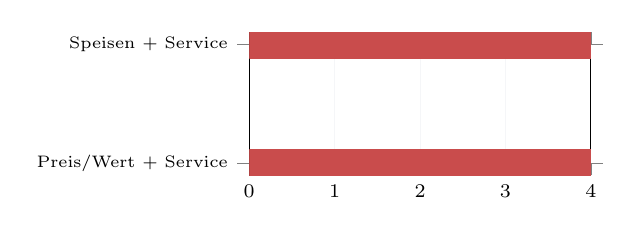
\begin{tikzpicture}\begin{axis}[xbar,width=5.92cm,height=3.4cm,xmin=0,xmax=4,symbolic y coords={Price+Service,Food+Service},ytick=data,yticklabels={Preis/Wert + Service,Speisen + Service},y tick label style={font=\fontsize{6.1}{7.1}\selectfont},xtick={0,1,2,3,4},xticklabel style={font=\scriptsize},grid=major,grid style={LightGray}]\addplot[fill=Red,draw=Red] coordinates {(\LowPairTwoCount,Price+Service) (\LowPairOneCount,Food+Service)};\end{axis}\end{tikzpicture}\par{\fontsize{7}{8.4}\selectfont Alle anderen Paare treten einmal auf. Gemeinsame Nennungen lenken interne Prüfungen, beweisen aber keine Ursache. Tages-, Uhrzeit- und Schichtdaten fehlen.}\end{columns}
  \vfill\goldbutton{a-bad-patterns}{Vollständige Muster anzeigen}\quad\redbutton{a-bad-cooccurrence}{Jüngste Verschiebung anzeigen}
\end{frame}

\begin{frame}{Jede schlechte Bewertung als operativen Fall behandeln, nicht nur als Zitat}
  \hypertarget{m-badcases}{}\sectiontag{Kapitel 5 - Operativer Fallprozess}
  \begin{columns}[T,onlytextwidth]\column{0.31\textwidth}\colorbox{PaleRed}{\parbox[c][3.75cm][t]{0.92\linewidth}{\vspace{0.14cm}\smallcapslabel{Fallerfassung}\par\vspace{0.10cm}{\fontsize{8.2}{9.8}\selectfont Anonyme Fall-ID, Bewertung/Datum, positive und negative Themen, Artikel-/Buffet-/Getränke-/Kartenmerkmale, mit/ohne Text und öffentlicher Link zur Originalbewertung.}}}\column{0.31\textwidth}\colorbox{PaleGold}{\parbox[c][3.75cm][t]{0.92\linewidth}{\vspace{0.14cm}\smallcapslabel{Zuständigkeit}\par\vspace{0.10cm}{\fontsize{8.2}{9.8}\selectfont Vorgeschlagene Zuständigkeit, 48-Stunden-Ziel für die öffentliche Antwort, problemspezifische interne Prüfung und Antwortdatum, sofern vorhanden.}}}\column{0.31\textwidth}\colorbox{PaleTeal}{\parbox[c][3.75cm][t]{0.92\linewidth}{\vspace{0.14cm}\smallcapslabel{Abschluss}\par\vspace{0.10cm}{\fontsize{8.2}{9.8}\selectfont Fall offen halten, bis interne Prüfung und Maßnahme dokumentiert sind. Felder zur internen Lösung sind derzeit nicht verfügbar.}}}\end{columns}
  \vfill\redbutton{a-bad-register}{30-Fälle-Register anzeigen}\quad\goldbutton{a-Antwort-process}{Antwortcheckliste anzeigen}
\end{frame}

\chapterdivider{6}{Service}{Der Service wird überwiegend positiv bewertet, ist aber die deutlichste wiederkehrende Schwäche bei niedrigen Bewertungen.}{Wiederholte Probleme bei Wartezeit, Reaktion und Kommunikation können viele positive Nennungen überlagern.}{Alle negativen Fälle nach Kontaktpunkt sowie künftig nach Schicht und Uhrzeit untersuchen.}{m-ch6}{Teal}

\begin{frame}{Der Service ist insgesamt positiv und bleibt dennoch die klarste wiederkehrende Schwäche}
  \hypertarget{m-ch6-content}{}\hypertarget{m-service}{}\sectiontag{Kapitel 6 - Service}
  \begin{columns}[T,onlytextwidth]\column{0.48\textwidth}\smallcapslabel{Historisch}\par\vspace{0.07cm}\countsentimentbar{\ServicePeriodHistoricalPositive}{\ServicePeriodHistoricalNeutral}{\ServicePeriodHistoricalNegative}\par{\color{Gray}\fontsize{6.7}{8}\selectfont \ServicePeriodHistoricalMentions\ Nennungen | \ServicePeriodHistoricalNegative\ negativ | \ServicePeriodHistoricalNegativeEvidence\ Schwächenevidenz}\par\vspace{0.15cm}\smallcapslabel{Letzte 90 Tage}\par\vspace{0.07cm}\countsentimentbar{\ServicePeriodRecentPositive}{\ServicePeriodRecentNeutral}{\ServicePeriodRecentNegative}\par{\color{Gray}\fontsize{6.7}{8}\selectfont \ServicePeriodRecentMentions\ Nennungen | \ServicePeriodRecentNegative\ negativ | \ServicePeriodRecentNegativeEvidence\ Schwächenevidenz}\par\vspace{0.15cm}{\fontsize{7.8}{9.3}\selectfont Letzte 30 Tage: \RecentThirtyServiceMentions\ Nennungen; \RecentThirtyServiceNegative\ negativ (\RecentThirtyServiceNegativeEvidence\ Evidenz). Strukturierte Bewertung: \ServiceRating.}\column{0.48\textwidth}\quoteneg{\QuoteServiceWaitText}{\QuoteServiceWaitMeta}\par\vspace{0.07cm}\quoteneg{\QuoteServiceOverwhelmedText}{\QuoteServiceOverwhelmedMeta}\par\vspace{0.07cm}\quotepos{\QuoteServicePositiveText}{\QuoteServicePositiveMeta}\end{columns}
  \vfill{\color{Gray}\fontsize{6.3}{7.5}\selectfont Historisch \EarliestReviewDate-\RecentNinetyStart; letzte 90 Tage \RecentNinetyStart-\LatestReviewDate; letzte 30 Tage \RecentThirtyStart-\LatestReviewDate.}\par\vspace{0.07cm}\redbutton{a-service}{Alle negativen Servicefälle anzeigen}
\end{frame}

\chapterdivider{7}{Küche / Speisen / Geschmack}{Speisen und Geschmack sind breite Stärken; jüngste Beschwerden mit geringem Volumen betreffen Qualität, Frische und Trockenheit.}{Starkes langfristiges Sentiment darf wenige, aber handlungsrelevante aktuelle Fälle nicht verdecken.}{Jede Beschwerde nach Gericht, Zubereitung, Warmhaltung sowie künftig Schicht und Uhrzeit prüfen.}{m-ch7}{Gold}

\begin{frame}{Speisen und Geschmack bleiben Stärken; jüngste Beschwerden brauchen eine Musterprüfung}
  \hypertarget{m-ch7-content}{}\hypertarget{m-food}{}\sectiontag{Kapitel 7 - Küche / Speisen / Geschmack}
  \begin{columns}[T,onlytextwidth]\column{0.48\textwidth}\smallcapslabel{Speisen: historisch / aktuell / zuletzt}\par{\fontsize{7.4}{8.8}\selectfont Historisch \FoodPeriodHistoricalMentions\ Nennungen, \FoodPeriodHistoricalNegative\ negativ (\FoodPeriodHistoricalNegativeEvidence). Letzte 90 Tage \FoodPeriodRecentMentions\, \FoodPeriodRecentNegative\ negativ (\FoodPeriodRecentNegativeEvidence). Letzte 30 Tage \RecentThirtyFoodMentions\, \RecentThirtyFoodNegative\ negativ (\RecentThirtyFoodNegativeEvidence).}\par\vspace{0.13cm}\smallcapslabel{Geschmack: historisch / aktuell / zuletzt}\par{\fontsize{7.4}{8.8}\selectfont Historisch \TastePeriodHistoricalMentions\ Nennungen, \TastePeriodHistoricalNegative\ negativ (\TastePeriodHistoricalNegativeEvidence). Letzte 90 Tage \TastePeriodRecentMentions\, \TastePeriodRecentNegative\ negativ (\TastePeriodRecentNegativeEvidence). Letzte 30 Tage \RecentThirtyTasteMentions\, \RecentThirtyTasteNegative\ negativ (\RecentThirtyTasteNegativeEvidence).}\column{0.48\textwidth}\quoteneg{\QuoteFoodStaleText}{\QuoteFoodStaleMeta}\par\vspace{0.07cm}\quoteneg{\QuoteTasteDryText}{\QuoteTasteDryMeta}\par\vspace{0.07cm}\quotepos{\QuoteFoodFreshText}{\QuoteFoodFreshMeta}\end{columns}
  \vfill{\color{Gray}\fontsize{6.3}{7.5}\selectfont Historisch \EarliestReviewDate-\RecentNinetyStart; letzte 90 Tage \RecentNinetyStart-\LatestReviewDate; letzte 30 Tage \RecentThirtyStart-\LatestReviewDate.}\par\vspace{0.07cm}\redbutton{a-food}{Alle negativen Speisen-/Geschmacksfälle anzeigen}
\end{frame}

\chapterdivider{8}{Bar \& Getränke}{Die Karte enthält 34 Getränkeartikel; nur zwei davon erhalten beobachtbare Aufmerksamkeit in Bewertungen.}{Geringe Aufmerksamkeit ist ein Sichtbarkeits- und Kontextsignal, keine Verkaufsaussage.}{Empfehlung, Präsentation und Bundles prüfen; Entscheidungen mit POS-Daten verknüpfen.}{m-ch8}{Teal}

\begin{frame}{Die Bar ist auf der Karte präsent, erhält aber wenig beobachtbare Aufmerksamkeit in Bewertungen}
  \hypertarget{m-ch8-content}{}\hypertarget{m-bar}{}\sectiontag{Kapitel 8 - Bar \& Getränke}
  \begin{columns}[T,onlytextwidth]\column{0.55\textwidth}\begin{tikzpicture}\begin{axis}[ybar stacked,bar width=24pt,width=8.0cm,height=4.45cm,symbolic x coords={0,1},xtick=data,xticklabels={Historisch,Letzte 90 Tage},x tick label style={font=\fontsize{6.5}{7.5}\selectfont},ytick={0,20,40,60,80,100},yticklabel style={font=\scriptsize},legend style={font=\fontsize{5.8}{6.8}\selectfont,at={(0.5,1.02)},anchor=south,legend columns=3,draw=none},grid=major,grid style={LightGray},ylabel={Sentimentanteil (\%)},ylabel style={font=\scriptsize}]\addplot[fill=Teal,draw=Teal] table[x=index,y=positive_pct,col sep=comma]{assets/bar_periods.csv};\addplot[fill=Gray!45,draw=Gray] table[x=index,y=neutral_pct,col sep=comma]{assets/bar_periods.csv};\addplot[fill=Red,draw=Red] table[x=index,y=negative_pct,col sep=comma]{assets/bar_periods.csv};\legend{Positiv,Neutral,Negativ}\end{axis}\end{tikzpicture}\column{0.41\textwidth}\smallcapslabel{Aufmerksamkeitsbasis}\par{\fontsize{7.6}{9.1}\selectfont Gesamtzeitraum \DrinkMentions\ Nennungen (\DrinkCoverage\% Abdeckung schriftlicher Bewertungen). \DrinkItemsMentioned/\DrinkMenuItems\ Getränkeartikel in Bewertungen beobachtet (\DrinkMenuCoverage\%). Letzte 30 Tage: \RecentThirtyDrinksMentions\ Nennungen; \RecentThirtyDrinksNegative\ negativ, \RecentThirtyDrinksNeutral\ neutral.}\par\vspace{0.12cm}\quotegray{\QuoteDrinkWrongText}{\QuoteDrinkWrongMeta}\end{columns}
  \vfill{\color{Gray}\fontsize{6.3}{7.5}\selectfont Historisch \EarliestReviewDate-\RecentNinetyStart; letzte 90 Tage \RecentNinetyStart-\LatestReviewDate. Aufmerksamkeit in Bewertungen ist nicht gleichbedeutend mit Verkaufszahlen.}\par\vspace{0.07cm}\goldbutton{a-bar}{Getränkebezogene Fälle anzeigen}
\end{frame}

\chapterdivider{9}{Buffet}{Insgesamt überwiegend positiv, aber die Evidenz zu Unterthemen ist dünn.}{Das Konzept ist operativ wichtig; Bewertungsdaten allein erlauben jedoch keine verlässliche Qualitätsdiagnose.}{Gezieltes Feedback erheben und Qualität, Preis-Leistung, Nachfüllung sowie Warteschlangen beobachten.}{m-ch9}{Gold}

\begin{frame}{Das Buffet wird insgesamt überwiegend positiv bewertet; die Evidenz zu Unterthemen ist jedoch dünn}
  \hypertarget{m-ch9-content}{}\hypertarget{m-buffet}{}\sectiontag{Kapitel 9 - Buffet}
  \begin{columns}[T,onlytextwidth]\column{0.48\textwidth}\begin{tikzpicture}\begin{axis}[ybar,bar width=24pt,width=6.8cm,height=4.2cm,symbolic x coords={Positive,Neutral,Negative},xtick=data,xticklabels={Positiv,Neutral,Negativ},x tick label style={font=\fontsize{6.5}{7.5}\selectfont},ytick={0,2,4,6,8,10,12},yticklabel style={font=\scriptsize},grid=major,grid style={LightGray},ylabel={Bewertungen},ylabel style={font=\scriptsize}]\addplot[fill=Gold,draw=Gold] table[x=sentiment,y=count,col sep=comma]{assets/buffet_sentiment.csv};\end{axis}\end{tikzpicture}\par{\color{Gray}\fontsize{6.2}{7.3}\selectfont Gesamtzeitraum \EarliestReviewDate-\LatestReviewDate: \BuffetReviews\ Nennungen, \BuffetCoverage\% Abdeckung schriftlicher Bewertungen.}\column{0.48\textwidth}\quotepos{\QuoteBuffetPositiveText}{\QuoteBuffetPositiveMeta}\par\vspace{0.07cm}\quoteneg{\QuoteBuffetNegativeText}{\QuoteBuffetNegativeMeta}\par\vspace{0.07cm}\quotegray{\QuoteBuffetNeutralText}{\QuoteBuffetNeutralMeta}\end{columns}
  \vfill{\fontsize{6.5}{7.7}\selectfont Qualität \BuffetQualityReviews\ | Auswahl \BuffetVarietyReviews\ | Frische \BuffetFreshnessReviews\ | Preis-Leistung \BuffetValueReviews\ | Nachfüllung \BuffetReplenishmentReviews\ | Warteschlange \BuffetWaitingQueueReviews. Unterthemen ohne stützende Bewertungen haben keine Evidenz, nicht niedrige Evidenz.}\par\vspace{0.07cm}\goldbutton{a-buffet}{Negative/neutrale Buffetfälle anzeigen}
\end{frame}

\chapterdivider{10}{Speisekarte \& Bestellung}{102 von 118 Kartenpositionen werden nicht erwähnt; daraus lassen sich weder Nachfrage noch Profitabilität ableiten.}{Streichungen oder Neugestaltung allein auf Basis von Bewertungserwähnungen würden Erinnerung mit Absatz verwechseln.}{Saubere POS-Kennzahlen erheben, Hypothesen bilden und anschließend kontrolliert testen.}{m-ch10}{Teal}

\begin{frame}{Fehlende Erwähnungen sind ein Speisekartensignal, keine Streichentscheidung}
  \hypertarget{m-ch10-content}{}\hypertarget{m-menu}{}\sectiontag{Kapitel 10 - Speisekarte \& Bestellung}
  \begin{columns}[T,onlytextwidth]\column{0.34\textwidth}\smallcapslabel{Was Bewertungen zeigen}\par\vspace{0.06cm}{\fontsize{7.5}{9}\selectfont \MenuItems\ Kartenpositionen; \MenuItemsMentioned\ mentioned; \MenuItemsUnmentioned\ ohne beobachtbare Nennung; \MenuAttentionCoverage\% Aufmerksamkeitsabdeckung. Bewertungen zeigen Erinnerung, Lob, Beschwerden und Orientierungshürden.}\par\vspace{0.13cm}\smallcapslabel{Was Bewertungen nicht zeigen}\par\vspace{0.06cm}{\fontsize{7.5}{9}\selectfont Bestellungen, Wiederkäufe, Umsatz, Marge, Retouren, Zeitmuster oder operative Komplexität.}\column{0.34\textwidth}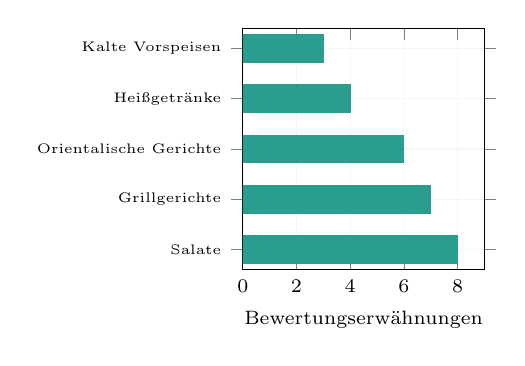
\begin{tikzpicture}\begin{axis}[xbar,width=4.65cm,height=4.65cm,xmin=0,xmax=9,ytick={0,1,2,3,4},yticklabels={\MenuCategoryOneName,\MenuCategoryTwoName,\MenuCategoryThreeName,\MenuCategoryFourName,\MenuCategoryFiveName},y tick label style={font=\fontsize{5.2}{6.2}\selectfont},xtick={0,2,4,6,8},xticklabel style={font=\scriptsize},grid=major,grid style={LightGray},xlabel={Bewertungserwähnungen},xlabel style={font=\scriptsize}]\addplot[fill=Teal,draw=Teal] coordinates {(\MenuCategoryOneMentions,0) (\MenuCategoryTwoMentions,1) (\MenuCategoryThreeMentions,2) (\MenuCategoryFourMentions,3) (\MenuCategoryFiveMentions,4)};\end{axis}\end{tikzpicture}\column{0.28\textwidth}\smallcapslabel{Entscheidungsmatrix}\par\vspace{0.06cm}{\fontsize{7.1}{8.5}\selectfont\textbf{Hohe Bestellungen / hohe Aufmerksamkeit}\par schützen und hervorheben\par\vspace{0.08cm}\textbf{Hoch / niedrig}\par Darstellung verbessern\par\vspace{0.08cm}\textbf{Niedrig / hoch}\par Polarisierung untersuchen\par\vspace{0.08cm}\textbf{Niedrig / niedrig}\par erst nach Margenprüfung vereinfachen}\end{columns}
  \vfill{\color{Gray}\fontsize{6.3}{7.5}\selectfont Bewertungszeitraum \EarliestReviewDate-\LatestReviewDate. POS-/Bestelldaten sind nicht verfügbar. Woche 2 bereitet Daten und Hypothesen vor; sie schließt keine Neugestaltung ab.}\par\vspace{0.07cm}\goldbutton{a-menu}{Beschwerdefälle zur Speisekarte anzeigen}\quad\tealbutton{a-pos}{POS-Felder und Matrix anzeigen}
\end{frame}

\chapterdivider{11}{In Bewertungen erwähnte Gerichte}{Sechzehn Gerichte bzw. Artikel haben beobachtbare Erwähnungen; nur Mansaf und Tabbouleh erfüllen die Schwelle von fünf Bewertungen.}{Ein Vergleich von zwei Artikeln trägt keine Best-/Schlechtestaussage, und Erwähnungen sind keine Bestellungen.}{Artikelebene als Hypothesen nutzen und mit POS-Daten verknüpfen.}{m-ch11}{Gold}

\begin{frame}{Gerichtevidenz zeigt Aufmerksamkeit und Einzelfälle, keine Bestseller}
  \hypertarget{m-ch11-content}{}\hypertarget{m-dishes}{}\sectiontag{Kapitel 11 - In Bewertungen erwähnte Gerichte}
  \begin{columns}[T,onlytextwidth]\column{0.53\textwidth}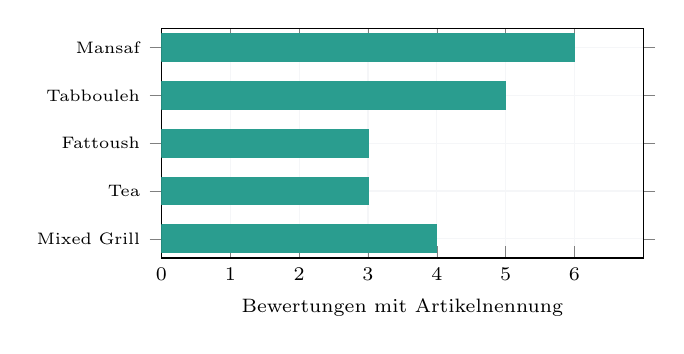
\begin{tikzpicture}\begin{axis}[xbar,width=7.7cm,height=4.5cm,xmin=0,xmax=7,symbolic y coords={MixedGrill,Tea,Fattoush,Tabbouleh,Mansaf},xtick={0,1,2,3,4,5,6},ytick=data,yticklabels={Mixed Grill,Tea,Fattoush,Tabbouleh,Mansaf},y tick label style={font=\fontsize{6.2}{7.2}\selectfont},xticklabel style={font=\scriptsize},grid=major,grid style={LightGray},xlabel={Bewertungen mit Artikelnennung},xlabel style={font=\scriptsize}]\addplot[fill=Teal,draw=Teal] coordinates {(\DiscussedDishThreeMentions,MixedGrill) (\DiscussedDishFiveMentions,Tea) (\DiscussedDishFourMentions,Fattoush) (\DiscussedDishTwoMentions,Tabbouleh) (\DiscussedDishOneMentions,Mansaf)};\end{axis}\end{tikzpicture}\column{0.43\textwidth}\smallcapslabel{Nach Bewertungsschwelle qualifiziert}\par{\fontsize{7.5}{9}\selectfont Mansaf \MansafMentions\ Nennungen, Durchschnitt der Gesamtbewertung \MansafReviewAverage; Tabbouleh \TabboulehMentions, Durchschnitt \TabboulehReviewAverage. Weniger als drei Gerichte qualifizieren sich; daher wird keine vergleichende Höchst-/Niedrigstplatzierung gezeigt.}\par\vspace{0.12cm}\smallcapslabel{Negative Artikelevidenz}\par{\fontsize{7.5}{9}\selectfont Mixed Grill: \MixedGrillMentions\ Nennungen, \MixedGrillNegative\ negativ; Durchschnitt der Gesamtbewertung \MixedGrillReviewAverage; \MixedGrillEvidence\ Evidenz.}\end{columns}
  \vfill{\color{Gray}\fontsize{6.3}{7.5}\selectfont Bewertungszeitraum \EarliestReviewDate-\LatestReviewDate. Die Gesamtbewertung ist keine garantierte gerichtsspezifische Bewertung.}\par\vspace{0.07cm}\goldbutton{a-dishes}{Alle 16 Gerichte/Artikel anzeigen}
\end{frame}

\chapterdivider{12}{Managementbeobachtungen}{Kundenevidenz, interne Beobachtungen, Datenbedarf, Experimente und Empfehlungen sind unterschiedliche Quellen.}{Vermischte Herkunft kann Hypothesen wie Fakten erscheinen lassen.}{Jede Aussage kennzeichnen und Experimente ausdrücklich freigeben.}{m-ch12}{Teal}

\begin{frame}{Evidenz, Beobachtungen, Experimente und Entscheidungen trennen}
  \hypertarget{m-ch12-content}{}\hypertarget{m-observations}{}\sectiontag{Kapitel 12 - Managementbeobachtungen}
  \begin{columns}[T,onlytextwidth]\column{0.48\textwidth}\sourceReview\par\vspace{0.06cm}{\fontsize{7.6}{9.1}\selectfont Getränke/Bar erhalten wenig beobachtbare Aufmerksamkeit; Verwirrung bei Karte/Tablet erscheint in der Kundenevidenz.}\par\vspace{0.13cm}\sourceInternal\par\vspace{0.06cm}{\fontsize{7.6}{9.1}\selectfont Statische Karte, manuelle Favoriten, fehlende wiederkehrende Angebote/Bundles, Parksichtbarkeit und aktuelle Begrüßung/Beratung sind Geschäftsbeobachtungen.}\par\vspace{0.13cm}\sourceExperiment\par\vspace{0.06cm}{\fontsize{7.6}{9.1}\selectfont Begrüßungsgeste, Wochenempfehlung, Bundle, Getränkefokus und bessere Gerichtmedien sind Tests.}\column{0.48\textwidth}\sourceData\par\vspace{0.06cm}{\fontsize{7.6}{9.1}\selectfont POS-Bestellungen, Umsatz, Marge, Retouren und Zeitmuster werden benötigt.}\par\vspace{0.13cm}\badge{PaleTeal}{MANAGEMENTMASSNAHME}\par\vspace{0.06cm}{\fontsize{7.6}{9.1}\selectfont Das Buffet benötigt gezieltes Feedback und Qualitätsmonitoring.}\par\vspace{0.13cm}\badge{PaleGold}{MESSPRINZIP}\par\vspace{0.06cm}{\fontsize{7.6}{9.1}\selectfont Die Gesamtbewertung verändert sich langsam; wöchentlich mit rollierenden 30-/90-Tage-Werten steuern.}\end{columns}
  \vfill\goldbutton{a-observations}{Herkunftsregister anzeigen}
\end{frame}

\chapterdivider{13}{Aktionsplan}{Sofortige Wiederherstellung ist von evidenzabhängigen Änderungen an Karte und Betrieb zu trennen.}{Eine verfrühte Neugestaltung würde der POS-Datenreife vorgreifen und Verantwortlichkeiten verdecken.}{Woche 1 jetzt umsetzen; Woche 2 für Daten und Hypothesen nutzen; anschließend testen und entscheiden.}{m-ch13}{Gold}

\begin{frame}{Sofortmaßnahmen von evidenzabhängigen Änderungen trennen}
  \hypertarget{m-ch13-content}{}\hypertarget{m-actions}{}\sectiontag{Kapitel 13 - Aktionsplan}
  \begin{columns}[T,onlytextwidth]\column{0.48\textwidth}\colorbox{PaleRed}{\parbox[c][4.45cm][t]{0.94\linewidth}{\vspace{0.13cm}{\color{Red}\fontsize{13}{15}\selectfont\bfseries Sofort}\par\vspace{0.10cm}\begin{itemize}\setlength\itemsep{0.07cm}\fontsize{7.8}{9.3}\selectfont\item Antwortverantwortung festlegen und Fälle protokollieren\item Offene aktuelle Bewertungen beantworten\item Service-/Speisenfälle prüfen\item Rollierendes KPI-Dashboard starten\item Team zur Beratung bei Karte, Buffet und Getränken briefen\item Wettbewerber-/Marktverkostungen zuweisen\end{itemize}\vfill\redbutton{a-actions}{Sofortcheckliste öffnen}}}\column{0.48\textwidth}\colorbox{PaleTeal}{\parbox[c][4.45cm][t]{0.94\linewidth}{\vspace{0.13cm}{\color{Teal}\fontsize{13}{15}\selectfont\bfseries Evidenzabhängig}\par\vspace{0.10cm}\begin{itemize}\setlength\itemsep{0.07cm}\fontsize{7.8}{9.3}\selectfont\item Woche 2: POS-Daten exportieren/bereinigen\item Felder und Neugestaltungshypothesen definieren\item Methode zur Favoritenauswahl definieren\item Erste kontrollierte Tests auswählen\item Wochen 3-4: testen, prüfen, entscheiden\item Marktcheck wiederholen und Evidenz vergleichen\end{itemize}\vfill\tealbutton{a-week2}{Plan für Woche 2 öffnen}}}\end{columns}
  \vfill\goldbutton{a-market-scan}{Wettbewerber-/Marktauftrag anzeigen}\quad\tealbutton{a-tests}{Test- und Entscheidungsplan anzeigen}
\end{frame}

\chapterdivider{14}{Delegation \& Zuständigkeit}{Sieben fragmentierte Arbeitsstränge lassen sich in vier verantwortliche Bereiche bündeln.}{Klare Zuständigkeit reduziert Übergaben, ohne die Managementverantwortung zu mindern.}{Ergebnisse und KPIs delegieren; Evidenz, Hindernisse und Termine wöchentlich prüfen.}{m-ch14}{Teal}

\begin{frame}{Vier Arbeitsbereiche; die Gesamtverantwortung bleibt beim Management}
  \hypertarget{m-ch14-content}{}\hypertarget{m-delegation}{}\sectiontag{Kapitel 14 - Delegation \& Zuständigkeit}
  \begin{columns}[T,onlytextwidth]\column{0.48\textwidth}\colorbox{PaleGold}{\parbox[c][1.81cm][t]{0.94\linewidth}{\vspace{0.06cm}\textbf{1. Reputation \& Daten}\par{\fontsize{7}{8.3}\selectfont Bewertungen, Antworten, Fälle, Dashboard und Evidenz. Zuständig: Administration/Marketing oder Management.}}}\par\vspace{0.06cm}\colorbox{PaleTeal}{\parbox[c][1.81cm][t]{0.94\linewidth}{\vspace{0.06cm}\textbf{2. Gästeerlebnis}\par{\fontsize{7}{8.3}\selectfont Begrüßung, Kartenberatung, Warten, Kommunikation und Buffetservice. Zuständig: Serviceleitung.}}}\column{0.48\textwidth}\colorbox{PaleRed}{\parbox[c][1.81cm][t]{0.94\linewidth}{\vspace{0.06cm}\textbf{3. Küche \& Buffetqualität}\par{\fontsize{7}{8.3}\selectfont Speisenfälle, Gerichtequalität, Frische, Konsistenz und Buffetkontrollen. Zuständig: Küchenleitung.}}}\par\vspace{0.06cm}\colorbox{LightGray}{\parbox[c][1.81cm][t]{0.94\linewidth}{\vspace{0.06cm}\textbf{4. Speisekarte, Bar \& Angebote}\par{\fontsize{7}{8.3}\selectfont POS-Analyse, Hypothesen, Favoriten, Angebote, Getränke und Medien. Zuständig: Management + Bereichsleitung.}}}\end{columns}
  \vfill\implication{Zuständigkeit delegieren, nicht Gesamtverantwortung. Das Management prüft wöchentlich Ergebnis, Evidenz, Hindernis, nächste Maßnahme und Frist.}\par\vspace{0.07cm}\goldbutton{a-workstreams}{Verantwortlichkeiten, KPIs und Eskalation anzeigen}
\end{frame}

\chapterdivider{15}{KPI-Steuerung}{Die wöchentliche Steuerung braucht rollierende Bewertungs-, Nachverfolgungs-, Betriebs- und Experimentkennzahlen.}{Die langfristige Google-Bewertung verändert sich zu langsam für die wöchentliche Steuerung.}{Aktuelle 30-Tage-Basis verwenden und rollierende 30-/90-Tage-Werte wöchentlich prüfen.}{m-ch15}{Gold}

\begin{frame}{Wöchentliches KPI-Dashboard: vier Steuerungsblöcke}
  \hypertarget{m-ch15-content}{}\hypertarget{m-kpi}{}\sectiontag{Kapitel 15 - KPI-Steuerung}
  \begin{columns}[T,onlytextwidth]\column{0.48\textwidth}\colorbox{PaleTeal}{\parbox[c][2.0cm][t]{0.94\linewidth}{\vspace{0.09cm}\smallcapslabel{1. Wöchentliche Bewertungs-KPIs}\par{\fontsize{7.2}{8.6}\selectfont Neue Bewertungen; Durchschnitt neuer Bewertungen; Negativanteil; Fälle mit niedriger Punktzahl. \textbf{Baseline:} \RecentThirtyPerWeek/Woche, \RecentThirtyAverage\ Durchschnitt, \RecentThirtyNegativePct\% negativ.}}}\par\vspace{0.10cm}\colorbox{PaleGold}{\parbox[c][2.0cm][t]{0.94\linewidth}{\vspace{0.09cm}\smallcapslabel{2. Nachverfolgungs-KPIs}\par{\fontsize{7.2}{8.6}\selectfont Antwortrate; Antworten auf niedrige Bewertungen; Verzögerung; offene Fälle. \textbf{Baseline:} \OwnerRecentThirtyRate\% aktuelle Antworten.}}}\column{0.48\textwidth}\colorbox{PaleRed}{\parbox[c][2.0cm][t]{0.94\linewidth}{\vspace{0.09cm}\smallcapslabel{3. Operative KPIs}\par{\fontsize{7.2}{8.6}\selectfont Negative Service- und Speisen-/Geschmacksfälle; Kartenbeschwerden; Getränkeaufmerksamkeit; Buffetsentiment. Anzahl, Anteil und Evidenz zeigen.}}}\par\vspace{0.10cm}\colorbox{LightGray}{\parbox[c][2.0cm][t]{0.94\linewidth}{\vspace{0.09cm}\smallcapslabel{4. Experiment-KPIs}\par{\fontsize{7.2}{8.6}\selectfont Nutzung von Angeboten/Bundles; Begrüßungsfeedback; geeignete Bestellungen; Umsatz/Marge; POS-/Bestellwirkung. Bis Testbeginn nicht verfügbar.}}}\end{columns}
  \vfill\colorbox{Navy}{\parbox{0.965\linewidth}{\color{white}\fontsize{7.4}{8.8}\selectfont Die langfristige Google-Bewertung verändert sich langsam. Für schnelles Feedback rollierende 30 Tage und für Stabilität 90 Tage nutzen; Gesamtwert monatlich prüfen.}}\par\vspace{0.07cm}\goldbutton{a-kpi}{KPI-Definitionen anzeigen}
\end{frame}

\chapterdivider{16}{Evidenzanhang}{Die Managementaussagen sind auf datierte Register, Diagramme, anonyme Auszüge und öffentliche Bewertungslinks zurückführbar.}{Entscheider können Details prüfen, ohne die Kernaussage zu überladen.}{Den passenden Anhang öffnen und anschließend zur Ausgangsfolie zurückkehren.}{m-ch16}{Teal}

\begin{frame}{Übersicht Evidenzanhang - Leistung und Fälle}
  \hypertarget{m-ch16-content}{}\hypertarget{a-index}{}\sectiontag{Kapitel 16 - Evidenzanhang}
  \begin{columns}[T,onlytextwidth]\column{0.48\textwidth}{\fontsize{7.2}{8.6}\selectfont\textbf{Anhang A - Letzte 30 Tage}\par Zusammenfassung sowie alle 14 Fälle mit Themen, Sprache, Antwort und Originallinks.\par\vspace{0.13cm}\textbf{Anhang B - Vorherige 30 Tage}\par Alle sechs Vergleichsfälle mit denselben Feldern.\par\vspace{0.13cm}\textbf{Anhang C - Register niedriger Bewertungen}\par Alle 30 Fälle mit niedriger Punktzahl samt vorgeschlagener Zuständigkeit, Frist, Prüfung und Abschlussstatus.\par\vspace{0.13cm}\textbf{Anhang D - Muster niedriger Bewertungen}\par Bereiche, gemeinsame Nennungen, aktuelle Verschiebung und Datenlücken.}\column{0.48\textwidth}{\fontsize{7.2}{8.6}\selectfont\textbf{Anhang E - Service}\par Alle negativen Servicefälle.\par\vspace{0.13cm}\textbf{Anhang F - Speisen/Geschmack}\par Alle negativen Fälle zu Speisen, Geschmack und Qualität.\par\vspace{0.13cm}\textbf{Anhang G - Bar/Getränke}\par Negative und neutrale Getränkefälle.\par\vspace{0.13cm}\textbf{Anhang H - Buffet}\par Negative und neutrale Buffetfälle.}\end{columns}
  \vfill\redbutton{a-bad-register}{30 Fälle niedriger Bewertungen öffnen}\quad\tealbutton{a-zuletzt-register}{Die letzten 14 Fälle öffnen}\quad\goldbutton{a-service}{Serviceevidenz öffnen}
\end{frame}

\begin{frame}{Übersicht Evidenzanhang - Betrieb und Maßnahmen}
  \hypertarget{m-appendix-roadmap-2}{}\sectiontag{Kapitel 16 - Evidenzanhang}
  \begin{columns}[T,onlytextwidth]\column{0.48\textwidth}{\fontsize{7.2}{8.6}\selectfont\textbf{Anhang I - Speisekarte/Tablet}\par Beschwerde- und neutrale Fälle.\par\vspace{0.13cm}\textbf{Anhang J - Gerichte/Artikel}\par Alle 16 Artikel mit Anzahlen, Sentiment, Durchschnitt, Evidenz, jüngstem Datum, Auszug und Link.\par\vspace{0.13cm}\textbf{Anhang K - Inhaberantwort}\par Periodendiagramm, Verzögerung und Antworten auf niedrige Bewertungen.\par\vspace{0.13cm}\textbf{Anhang L - Herkunft}\par Korrigierte Kennzeichnungen für Evidenz, Beobachtung und Maßnahme.}\column{0.48\textwidth}{\fontsize{7.2}{8.6}\selectfont\textbf{Anhang M - Maßnahmensystem}\par Sofortcheckliste; Datenaufbau in Woche 2; Tests; Marktprüfung; vier Arbeitsbereiche; Antwortprozess; POS-Matrix.\par\vspace{0.13cm}\textbf{Anhang N - KPI-Steuerung}\par Definitionen, Frequenz, Zuständigkeit und Ausgangswert.\par\vspace{0.20cm}\colorbox{PaleGold}{\parbox{0.92\linewidth}{\fontsize{7}{8.4}\selectfont Gold = Evidenz-/Maßnahmendetail. Türkis = Fall-/Datendetail. Rot = Register niedriger Bewertungen. Jede Anhangsseite hat eine sichtbare Zurück-Schaltfläche.}}}\end{columns}
  \vfill\goldbutton{a-dishes}{Alle Gerichte öffnen}\quad\tealbutton{a-actions}{Maßnahmencheckliste öffnen}\quad\backbutton{m-roadmap}{Zurück zur Präsentationsübersicht}
\end{frame}

% Generated by presentation/build_presentation.py. Do not edit manually.
\begin{frame}{Anhang O - Monatliche Trendevidenz}
  \hypertarget{a-trend}{}\appendixhead{O - Trends}
  {\color{Gray}\fontsize{6.3}{7.5}\selectfont Datensatz \EarliestReviewDate\ bis \LatestReviewDate. Dez. 2024 und Sep. 2026 sind unvollständig; alle dazwischenliegenden Monate sind vollständig.}
  \vspace{0.08cm}\begin{columns}[T,onlytextwidth]\column{0.33\textwidth}\smallcapslabel{Durchschnittsbewertung}\par\begin{tikzpicture}\begin{axis}[width=4.65cm,height=3.85cm,xmin=-.5,xmax=21.5,ymin=2.4,ymax=5.15,monthly axis ticks,x tick label style={font=\fontsize{4.6}{5.5}\selectfont,rotate=35,anchor=east},ytick={3,4,5},yticklabel style={font=\tiny},grid=major,grid style={LightGray}]\addplot[Navy,thick,mark=*,mark size=1pt] table[x=index,y=average,col sep=comma]{assets/monthly_trend.csv};\addplot[Gold,only marks,mark=*,mark size=3pt] table[x=index,y=average,col sep=comma]{assets/monthly_partial.csv};\end{axis}\end{tikzpicture}\column{0.33\textwidth}\smallcapslabel{Bewertungsvolumen}\par\begin{tikzpicture}\begin{axis}[ybar,bar width=3pt,width=4.65cm,height=3.85cm,xmin=-.5,xmax=21.5,ymin=0,ymax=24,monthly axis ticks,x tick label style={font=\fontsize{4.6}{5.5}\selectfont,rotate=35,anchor=east},ytick={0,10,20},yticklabel style={font=\tiny},grid=major,grid style={LightGray}]\addplot[fill=Teal,draw=Teal] table[x=index,y=reviews,col sep=comma]{assets/review_volume.csv};\end{axis}\end{tikzpicture}\column{0.33\textwidth}\smallcapslabel{Volumen niedriger Bewertungen}\par\begin{tikzpicture}\begin{axis}[ybar,bar width=3pt,width=4.65cm,height=3.85cm,xmin=-.5,xmax=21.5,ymin=0,ymax=6,monthly axis ticks,x tick label style={font=\fontsize{4.6}{5.5}\selectfont,rotate=35,anchor=east},ytick={0,2,4,6},yticklabel style={font=\tiny},grid=major,grid style={LightGray}]\addplot[fill=Red,draw=Red] table[x=index,y=low_scores,col sep=comma]{assets/monthly_trend.csv};\end{axis}\end{tikzpicture}\end{columns}
  \vfill\implication{Bewertung zusammen mit Volumen und niedrigen Bewertungen lesen; unvollständige Monate sind nicht mit vollen Monatssummen vergleichbar.}\par\vspace{0.07cm}\backbutton{m-trend}{Zurück zu Leistungstrends}
\end{frame}

\begin{frame}{Anhang A1 - Letzte 30 Tage: Detailvergleich}
  \hypertarget{a-zuletzt-summary}{}\appendixhead{A1 - Zusammenfassung letzte 30 Tage}
  {\color{Gray}\fontsize{6.5}{7.7}\selectfont Letzte 30 Tage: \RecentThirtyStart\ bis \LatestReviewDate. Vorherige 30 Tage: \PreviousThirtyStart\ bis \RecentThirtyStart.}
  \vspace{0.10cm}\begin{columns}[T,onlytextwidth]
    \column{0.43\textwidth}\smallcapslabel{Zeitraumübersicht}\par\vspace{0.07cm}{\fontsize{7.6}{9.1}\selectfont Aktuell: \RecentThirtyReviews\ Bewertungen / \RecentThirtyWritten\ mit Text / Durchschnitt \RecentThirtyAverage\ / \RecentThirtyNegativePct\% negativ / \RecentThirtyLowScores\ niedrige Punktzahl / \OwnerRecentThirtyRate\% Antwort.\par\vspace{0.10cm}Vorher: \PreviousThirtyReviews\ Bewertungen / \PreviousThirtyWritten\ mit Text / Durchschnitt \PreviousThirtyAverage\ / \PreviousThirtyNegativePct\% negativ / \PreviousThirtyLowScores\ niedrige Punktzahl / \OwnerPreviousThirtyRate\% Antwort.\par\vspace{0.10cm}Speisen, Service, Geschmack, Getränke, Buffet und Speisekarte/Tablet werden rechts verglichen; gezählt werden eindeutige Bewertungen, keine Phrasen.}
    \column{0.53\textwidth}\begin{tikzpicture}\begin{axis}[ybar,bar width=4pt,width=7.6cm,height=4.35cm,symbolic x coords={Food,Service,Taste,Drinks,Buffet,Menu & Tablet,Atmosphere,Staff Friendliness,Staff Communication,Parking},xtick=data,xticklabels={Speisen,Service,Geschmack,Getränke,Buffet,Speisekarte,Atmosphäre,Friendliness,Communication,Parken},x tick label style={font=\fontsize{5.3}{6.3}\selectfont,rotate=30,anchor=east},ytick={0,1,2,3,4,5,6},yticklabel style={font=\scriptsize},legend style={font=\fontsize{5.8}{6.8}\selectfont,at={(0.5,1.02)},anchor=south,legend columns=2,draw=none},grid=major,grid style={LightGray}]\addplot[fill=Teal,draw=Teal] table[x=topic,y=recent_mentions,col sep=comma]{assets/last_30d_topics.csv};\addplot[fill=Gray!50,draw=Gray] table[x=topic,y=previous_mentions,col sep=comma]{assets/last_30d_topics.csv};\legend{Aktuell,Vorher}\end{axis}\end{tikzpicture}
  \end{columns}\vfill\backbutton{m-lastmonth}{Zurück zur Monatsentwicklung}\quad\tealbutton{a-zuletzt-register}{Alle 14 Fälle öffnen}
\end{frame}

\begin{frame}{Anhang A2 - Fallregister der letzten 30 Tage}
  \hypertarget{a-zuletzt-register}{}\appendixhead{A2 - Fälle 1-2 von 14}
  \casecard{L01}{03 Sep 2026 | 5 Sterne | mit Text | Englisch | keine Übersetzung erforderlich | Inhaberantwort nein}{Negativ: keine erkannt; Positiv: Atmosphäre, Speisen, Gastfreundschaft, Service +1; Neutral: keine erkannt.}{Artikel: keine erkannt; Buffet nein; Getränke nein; Karte/Tablet nein; Service ja; Preis-Leistung nein.}{Eine wunderbare Entdeckung: Das Essen war köstlich, und das Personal war freundlich und herzlich. Die Atmosphäre mit orientalischem Flair war großartig.}{\href{https://www.google.com/maps/Bewertungen/data=!4m8!14m7!1m6!2m5!1sCi9DQUlRQUNvZENodHljRjlvT21GVlJVSmxNalpHV0hBNFdtaE5OV1ZoV0d4TVZrRRAB!2m1!1s0x0:0x27a031a79977995f!3m1!1s2@1:CAIQACodChtycF9oOmFVRUJlMjZGWHA4WmhNNWVhWGxMVkE\%7C\%7C?hl=en}{\color{Teal}\fontsize{6.1}{7.2}\selectfont\bfseries Originalbewertung öffnen $\rightarrow$}}
  \casecard{L02}{31 Aug 2026 | 2 Sterne | mit Text | Deutsch | Übersetzung ja | Inhaberantwort nein}{Negativ: Speisen, Speisekarte \& Tablet, Parken, Service +2; Positiv: Komfort; Neutral: Buffet, Card Zahlung, Sauberkeit, Getränke +2.}{Artikel: keine erkannt; Buffet ja; Getränke ja; Karte/Tablet ja; Service ja; Preis-Leistung nein.}{Leider müssen wir unsere Bewertung aktualisieren. Die Qualität hat stark abgenommen, bei unserem letzten Besuch wurden weder Salz/Pfeffer noch Öl an den Tisch gebracht und geschmacklich hat ...}{\href{https://www.google.com/maps/Bewertungen/data=!4m8!14m7!1m6!2m5!1sChZDSUhNMG9nS0VKbnJfYUtMMi1yY1ZREAE!2m1!1s0x0:0x27a031a79977995f!3m1!1s2@1:CIHM0ogKEJnr\_aKL2-rcVQ\%7C\%7C?hl=en}{\color{Teal}\fontsize{6.1}{7.2}\selectfont\bfseries Originalbewertung öffnen $\rightarrow$}}
  \vfill\backbutton{m-lastmonth}{Zurück zur Monatsentwicklung}
\end{frame}

\begin{frame}{Anhang A3 - Fallregister der letzten 30 Tage}
  \hypertarget{a-zuletzt-3}{}\appendixhead{A3 - Fälle 3-4 von 14}
  \casecard{L03}{29 Aug 2026 | 4 Sterne | mit Text | Deutsch | Übersetzung ja | Inhaberantwort nein}{Negativ: keine erkannt; Positiv: Gastfreundschaft, Service; Neutral: keine erkannt.}{Artikel: keine erkannt; Buffet nein; Getränke nein; Karte/Tablet nein; Service ja; Preis-Leistung nein.}{Avin ? Top Service,danke für deine Gastfreundlichkeit. So wünscht man sich das heutzutage. Toller Abend.}{\href{https://www.google.com/maps/Bewertungen/data=!4m8!14m7!1m6!2m5!1sCi9DQUlRQUNvZENodHljRjlvT2tWWVpsVmtkVnBLUVZvMVlXOTJhM1JXWWtVMmJXYxAB!2m1!1s0x0:0x27a031a79977995f!3m1!1s2@1:CAIQACodChtycF9oOkVYZlVkdVpKQVo1YW92a3RWYkU2bWc\%7C\%7C?hl=en}{\color{Teal}\fontsize{6.1}{7.2}\selectfont\bfseries Originalbewertung öffnen $\rightarrow$}}
  \casecard{L04}{25 Aug 2026 | 4 Sterne | ohne Text | Unbekannt | Übersetzung nein | Inhaberantwort nein}{Negativ: keine erkannt; Positiv: keine erkannt; Neutral: keine erkannt.}{Artikel: keine erkannt; Buffet nein; Getränke nein; Karte/Tablet nein; Service nein; Preis-Leistung nein.}{Kein Bewertungstext verfügbar.}{\href{https://www.google.com/maps/Bewertungen/data=!4m8!14m7!1m6!2m5!1sCi9DQUlRQUNvZENodHljRjlvT2poT1VUVXhabU5rZFVOQ00yTnRWemxFVmpaRlpIYxAB!2m1!1s0x0:0x27a031a79977995f!3m1!1s2@1:CAIQACodChtycF9oOjhOUTUxZmNkdUNCM2NtVzlEVjZFZHc\%7C\%7C?hl=en}{\color{Teal}\fontsize{6.1}{7.2}\selectfont\bfseries Originalbewertung öffnen $\rightarrow$}}
  \vfill\backbutton{m-lastmonth}{Zurück zur Monatsentwicklung}
\end{frame}

\begin{frame}{Anhang A4 - Fallregister der letzten 30 Tage}
  \hypertarget{a-zuletzt-4}{}\appendixhead{A4 - Fälle 5-6 von 14}
  \casecard{L05}{25 Aug 2026 | 5 Sterne | mit Text | Deutsch | Übersetzung ja | Inhaberantwort nein}{Negativ: keine erkannt; Positiv: Atmosphäre, Buffet, Komfort, Speisen +7; Neutral: Speisenauswahl, Kommunikation des Personals.}{Artikel: keine erkannt; Buffet ja; Getränke nein; Karte/Tablet nein; Service ja; Preis-Leistung ja.}{Wir waren im Restaurant Al Assiel und waren rundum begeistert! Das Essen war sehr lecker und das Buffet wirklich hervorragend. Es ist sehr vielfältig und bietet eine ...}{\href{https://www.google.com/maps/Bewertungen/data=!4m8!14m7!1m6!2m5!1sCi9DQUlRQUNvZENodHljRjlvT2tGUVIzQTVSbXhSWlV0VVpXOXRSWFppWlRVd1VIYxAB!2m1!1s0x0:0x27a031a79977995f!3m1!1s2@1:CAIQACodChtycF9oOkFQR3A5RmxRZUtUZW9tRXZiZTUwUHc\%7C\%7C?hl=en}{\color{Teal}\fontsize{6.1}{7.2}\selectfont\bfseries Originalbewertung öffnen $\rightarrow$}}
  \casecard{L06}{22 Aug 2026 | 5 Sterne | mit Text | Deutsch | Übersetzung ja | Inhaberantwort nein}{Negativ: keine erkannt; Positiv: Atmosphäre, Buffet, Komfort, Service +2; Neutral: Shisha.}{Artikel: keine erkannt; Buffet ja; Getränke nein; Karte/Tablet nein; Service ja; Preis-Leistung nein.}{Tolles gemütliches Ambiente, Buffet war reichhaltig abwechslungsreich und sehr lecker. Dessert waren einfach köstlich. Zudem konnten wir Shisha rauchen.Das Personal war einfach nur mega lieb und freundlich.Wir ...}{\href{https://www.google.com/maps/Bewertungen/data=!4m8!14m7!1m6!2m5!1sCi9DQUlRQUNvZENodHljRjlvT2pGSU1uTkxWbXA0TjFOQlVYY3plRXBQTkc1SlZIYxAB!2m1!1s0x0:0x27a031a79977995f!3m1!1s2@1:CAIQACodChtycF9oOjFIMnNLVmp4N1NBUXczeEpPNG5JVHc\%7C\%7C?hl=en}{\color{Teal}\fontsize{6.1}{7.2}\selectfont\bfseries Originalbewertung öffnen $\rightarrow$}}
  \vfill\backbutton{m-lastmonth}{Zurück zur Monatsentwicklung}
\end{frame}

\begin{frame}{Anhang A5 - Fallregister der letzten 30 Tage}
  \hypertarget{a-zuletzt-5}{}\appendixhead{A5 - Fälle 7-8 von 14}
  \casecard{L07}{22 Aug 2026 | 5 Sterne | mit Text | Deutsch | Übersetzung ja | Inhaberantwort nein}{Negativ: keine erkannt; Positiv: Atmosphäre, Buffet, Speisen, Geschmack; Neutral: Gastfreundschaft, Service, Shisha.}{Artikel: keine erkannt; Buffet ja; Getränke nein; Karte/Tablet nein; Service ja; Preis-Leistung nein.}{Richtig schöne Ambiente am Wochenende Buffet. Richtig leckeres Essen kann ich nur empfehlen!!! Auch shisha gibt es hier !! Und man wird so herzlich empfangen. Super Service!}{\href{https://www.google.com/maps/Bewertungen/data=!4m8!14m7!1m6!2m5!1sCi9DQUlRQUNvZENodHljRjlvT2pGQmVrNTFNRTU0WVhWRWNsaHlabGR4ZUVkbFduYxAB!2m1!1s0x0:0x27a031a79977995f!3m1!1s2@1:CAIQACodChtycF9oOjFBek51ME54YXVEclhyZldxeEdlWnc\%7C\%7C?hl=en}{\color{Teal}\fontsize{6.1}{7.2}\selectfont\bfseries Originalbewertung öffnen $\rightarrow$}}
  \casecard{L08}{22 Aug 2026 | 2 Sterne | mit Text | Arabisch | Übersetzung ja | Inhaberantwort nein}{Negativ: keine erkannt; Positiv: Speisen, Service, Geschmack; Neutral: keine erkannt.}{Artikel: keine erkannt; Buffet nein; Getränke nein; Karte/Tablet nein; Service ja; Preis-Leistung nein.}{Köstliches Essen und guter Service.}{\href{https://www.google.com/maps/Bewertungen/data=!4m8!14m7!1m6!2m5!1sCi9DQUlRQUNvZENodHljRjlvT2s5MGNFdHVWVFkyTFRWNllVVllNbHBFUWtkdlZXYxAB!2m1!1s0x0:0x27a031a79977995f!3m1!1s2@1:CAIQACodChtycF9oOk90cEtuVTY2LTV6YUVYMlpEQkdvVWc\%7C\%7C?hl=en}{\color{Teal}\fontsize{6.1}{7.2}\selectfont\bfseries Originalbewertung öffnen $\rightarrow$}}
  \vfill\backbutton{m-lastmonth}{Zurück zur Monatsentwicklung}
\end{frame}

\begin{frame}{Anhang A6 - Fallregister der letzten 30 Tage}
  \hypertarget{a-zuletzt-6}{}\appendixhead{A6 - Fälle 9-10 von 14}
  \casecard{L09}{16 Aug 2026 | 5 Sterne | ohne Text | Unbekannt | Übersetzung nein | Inhaberantwort nein}{Negativ: keine erkannt; Positiv: keine erkannt; Neutral: keine erkannt.}{Artikel: keine erkannt; Buffet nein; Getränke nein; Karte/Tablet nein; Service nein; Preis-Leistung nein.}{Kein Bewertungstext verfügbar.}{\href{https://www.google.com/maps/Bewertungen/data=!4m8!14m7!1m6!2m5!1sCi9DQUlRQUNvZENodHljRjlvT2poNmJHZHFTalJFWWtkYWQzYzBZelppYld0dVFuYxAB!2m1!1s0x0:0x27a031a79977995f!3m1!1s2@1:CAIQACodChtycF9oOjh6bGdqSjREYkdad3c0YzZibWtuQnc\%7C\%7C?hl=en}{\color{Teal}\fontsize{6.1}{7.2}\selectfont\bfseries Originalbewertung öffnen $\rightarrow$}}
  \casecard{L10}{16 Aug 2026 | 5 Sterne | mit Text | Deutsch | Übersetzung ja | Inhaberantwort nein}{Negativ: keine erkannt; Positiv: Speisen, Service; Neutral: keine erkannt.}{Artikel: keine erkannt; Buffet nein; Getränke nein; Karte/Tablet nein; Service ja; Preis-Leistung nein.}{Wir waren da, ich würde gerne wieder hin super Service,,,,, super Essen ,}{\href{https://www.google.com/maps/Bewertungen/data=!4m8!14m7!1m6!2m5!1sCi9DQUlRQUNvZENodHljRjlvT2s1c1IzZDFPWFp1TWt4cllYaHZkelZKVmxwdk5VRRAB!2m1!1s0x0:0x27a031a79977995f!3m1!1s2@1:CAIQACodChtycF9oOk5sR3d1OXZuMkxrYXhvdzVJVlpvNUE\%7C\%7C?hl=en}{\color{Teal}\fontsize{6.1}{7.2}\selectfont\bfseries Originalbewertung öffnen $\rightarrow$}}
  \vfill\backbutton{m-lastmonth}{Zurück zur Monatsentwicklung}
\end{frame}

\begin{frame}{Anhang A7 - Fallregister der letzten 30 Tage}
  \hypertarget{a-zuletzt-7}{}\appendixhead{A7 - Fälle 11-12 von 14}
  \casecard{L11}{12 Aug 2026 | 2 Sterne | mit Text | Deutsch | Übersetzung ja | Inhaberantwort nein}{Negativ: Getränke, Wartezeit; Positiv: Geschmack; Neutral: Speisen, Service.}{Artikel: keine erkannt; Buffet nein; Getränke ja; Karte/Tablet nein; Service ja; Preis-Leistung nein.}{Essen kam nach über einer Stunde immnoch nicht war trozdem lecker. Der Service war okay haben aber das falsche Getränk bekommen.}{\href{https://www.google.com/maps/Bewertungen/data=!4m8!14m7!1m6!2m5!1sCi9DQUlRQUNvZENodHljRjlvT205UGNsZEdkbTlXUW10aVJUZGpjak5CY1hSQmFWRRAB!2m1!1s0x0:0x27a031a79977995f!3m1!1s2@1:CAIQACodChtycF9oOm9PcldGdm9WQmtiRTdjcjNBcXRBaVE\%7C\%7C?hl=en}{\color{Teal}\fontsize{6.1}{7.2}\selectfont\bfseries Originalbewertung öffnen $\rightarrow$}}
  \casecard{L12}{09 Aug 2026 | 5 Sterne | ohne Text | Unbekannt | Übersetzung nein | Inhaberantwort nein}{Negativ: keine erkannt; Positiv: keine erkannt; Neutral: keine erkannt.}{Artikel: keine erkannt; Buffet nein; Getränke nein; Karte/Tablet nein; Service nein; Preis-Leistung nein.}{Kein Bewertungstext verfügbar.}{\href{https://www.google.com/maps/Bewertungen/data=!4m8!14m7!1m6!2m5!1sCi9DQUlRQUNvZENodHljRjlvT21sVWJXVm9hWGxQV201Q1UxRk1hbE0wYWtabFRrRRAB!2m1!1s0x0:0x27a031a79977995f!3m1!1s2@1:CAIQACodChtycF9oOmlUbWVoaXlPWm5CU1FMalM0akZlTkE\%7C\%7C?hl=en}{\color{Teal}\fontsize{6.1}{7.2}\selectfont\bfseries Originalbewertung öffnen $\rightarrow$}}
  \vfill\backbutton{m-lastmonth}{Zurück zur Monatsentwicklung}
\end{frame}

\begin{frame}{Anhang A8 - Fallregister der letzten 30 Tage}
  \hypertarget{a-zuletzt-8}{}\appendixhead{A8 - Fälle 13-14 von 14}
  \casecard{L13}{08 Aug 2026 | 1 Stern | mit Text | Arabisch | Übersetzung ja | Inhaberantwort nein}{Negativ: Buffet, Speisen, Speisen Qualität, Speisenauswahl +1; Positiv: keine erkannt; Neutral: Buffetauswahl.}{Artikel: Fattoush, kibbeh; Buffet ja; Getränke nein; Karte/Tablet nein; Service nein; Preis-Leistung nein.}{Wir waren zu zweit und bestellten das offene Buffet. Leider waren die Speisen furchtbar und sehr abgestanden. Kein einziges Gericht wirkte frisch. Der Fattoush-Salat war alt und ...}{\href{https://www.google.com/maps/Bewertungen/data=!4m8!14m7!1m6!2m5!1sCi9DQUlRQUNvZENodHljRjlvT21Kc2VrbDZjRmQzWWpCWlJub3hjbXhqU1RoTE5IYxAB!2m1!1s0x0:0x27a031a79977995f!3m1!1s2@1:CAIQACodChtycF9oOmJsekl6cFd3YjBZRnoxcmxjSThLNHc\%7C\%7C?hl=en}{\color{Teal}\fontsize{6.1}{7.2}\selectfont\bfseries Originalbewertung öffnen $\rightarrow$}}
  \casecard{L14}{08 Aug 2026 | 5 Sterne | mit Text | Deutsch | Übersetzung ja | Inhaberantwort nein}{Negativ: keine erkannt; Positiv: Atmosphäre, Speisen, Anrichtung, Frische +5; Neutral: Speisen Qualität, Gastfreundschaft.}{Artikel: keine erkannt; Buffet nein; Getränke nein; Karte/Tablet ja; Service ja; Preis-Leistung nein.}{Das Essen war einfach ausgezeichnet - frisch zubereitet, geschmackvoll und sehr schön angerichtet. Man merkt sofort, dass hier viel Wert auf Qualität und frische Zutaten gelegt wird. ...}{\href{https://www.google.com/maps/Bewertungen/data=!4m8!14m7!1m6!2m5!1sCi9DQUlRQUNvZENodHljRjlvT21sVU1HZHhPV3g0UVZaU2FGSXhkWGRJV0hONU0zYxAB!2m1!1s0x0:0x27a031a79977995f!3m1!1s2@1:CAIQACodChtycF9oOmlUMGdxOWx4QVZSaFIxdXdIWHN5M3c\%7C\%7C?hl=en}{\color{Teal}\fontsize{6.1}{7.2}\selectfont\bfseries Originalbewertung öffnen $\rightarrow$}}
  \vfill\backbutton{m-lastmonth}{Zurück zur Monatsentwicklung}
\end{frame}

\begin{frame}{Anhang B1 - Fallregister der vorherigen 30 Tage}
  \hypertarget{a-previous-register}{}\appendixhead{B1 - Fälle 1-2 von 6}
  \casecard{P01}{04 Aug 2026 | 5 Sterne | mit Text | Deutsch | Übersetzung ja | Inhaberantwort nein}{Negativ: keine erkannt; Positiv: Speisen, Service, Freundlichkeit des Personals, Geschmack; Neutral: keine erkannt.}{Artikel: keine erkannt; Buffet nein; Getränke nein; Karte/Tablet nein; Service ja; Preis-Leistung nein.}{Wir waren dort zu zweit essen , es war so ein schöner Abend. Das Essen war unfassbar lecker und die Mitarbeiter waren sehr freundlich ! Es hat ...}{\href{https://www.google.com/maps/Bewertungen/data=!4m8!14m7!1m6!2m5!1sCi9DQUlRQUNvZENodHljRjlvT25WU1VVdGlSekZ1ZUdaSFdIcElMVmswWTNGamFuYxAB!2m1!1s0x0:0x27a031a79977995f!3m1!1s2@1:CAIQACodChtycF9oOnVSUUtiRzFueGZHWHpILVk0Y3Fjanc\%7C\%7C?hl=en}{\color{Teal}\fontsize{6.1}{7.2}\selectfont\bfseries Originalbewertung öffnen $\rightarrow$}}
  \casecard{P02}{01 Aug 2026 | 5 Sterne | ohne Text | Unbekannt | Übersetzung nein | Inhaberantwort nein}{Negativ: keine erkannt; Positiv: keine erkannt; Neutral: keine erkannt.}{Artikel: keine erkannt; Buffet nein; Getränke nein; Karte/Tablet nein; Service nein; Preis-Leistung nein.}{Kein Bewertungstext verfügbar.}{\href{https://www.google.com/maps/Bewertungen/data=!4m8!14m7!1m6!2m5!1sCi9DQUlRQUNvZENodHljRjlvT2tWdlpFbEJlbmhSUVZkVlZWQXhVMXB0VmxsUlJIYxAB!2m1!1s0x0:0x27a031a79977995f!3m1!1s2@1:CAIQACodChtycF9oOkVvZElBenhRQVdVVVAxU1ptVllRRHc\%7C\%7C?hl=en}{\color{Teal}\fontsize{6.1}{7.2}\selectfont\bfseries Originalbewertung öffnen $\rightarrow$}}
  \vfill\backbutton{m-lastmonth}{Zurück zur Monatsentwicklung}
\end{frame}

\begin{frame}{Anhang B2 - Fallregister der vorherigen 30 Tage}
  \hypertarget{a-previous-2}{}\appendixhead{B2 - Fälle 3-4 von 6}
  \casecard{P03}{29 Jul 2026 | 5 Sterne | mit Text | Arabisch | Übersetzung ja | Inhaberantwort nein}{Negativ: keine erkannt; Positiv: Atmosphäre, Buffet, Speisen, Preis-Leistungs-Verhältnis +1; Neutral: keine erkannt.}{Artikel: keine erkannt; Buffet ja; Getränke nein; Karte/Tablet nein; Service nein; Preis-Leistung ja.}{Das Essen ist köstlich und hervorragend, das Buffet bietet alles, und die Preise sind im Vergleich zu anderen Restaurants günstig. Ehrlich gesagt ist es hinsichtlich Essen und ...}{\href{https://www.google.com/maps/Bewertungen/data=!4m8!14m7!1m6!2m5!1sCi9DQUlRQUNvZENodHljRjlvT2tWaFZqVlVhVTgyYTFoMlkxbElabUYzTlVsTmEwRRAB!2m1!1s0x0:0x27a031a79977995f!3m1!1s2@1:CAIQACodChtycF9oOkVhVjVUaU82a1h2Y1lIZmF3NUlNa0E\%7C\%7C?hl=en}{\color{Teal}\fontsize{6.1}{7.2}\selectfont\bfseries Originalbewertung öffnen $\rightarrow$}}
  \casecard{P04}{28 Jul 2026 | 1 Stern | mit Text | Deutsch | Übersetzung ja | Inhaberantwort nein}{Negativ: Speisen, Speisen Qualität, Meat Qualität, Service +2; Positiv: keine erkannt; Neutral: Getränke.}{Artikel: Gemischte Grillplatte, burger; Buffet nein; Getränke ja; Karte/Tablet nein; Service ja; Preis-Leistung nein.}{Also Burger kam ohne Nachos. Bedienung war überfordert und unfreundlich. Getränke kamen nach der Vorspeise. Teller werden nicht abgeräumt es wird nach Ablage der Gerichte nicht mehr ...}{\href{https://www.google.com/maps/Bewertungen/data=!4m8!14m7!1m6!2m5!1sCi9DQUlRQUNvZENodHljRjlvT2xodWRYUnJabmw1Vld0aFZGVmpNMVF6WlhjMFZVRRAB!2m1!1s0x0:0x27a031a79977995f!3m1!1s2@1:CAIQACodChtycF9oOlhudXRrZnl5VWthVFVjM1QzZXc0VUE\%7C\%7C?hl=en}{\color{Teal}\fontsize{6.1}{7.2}\selectfont\bfseries Originalbewertung öffnen $\rightarrow$}}
  \vfill\backbutton{m-lastmonth}{Zurück zur Monatsentwicklung}
\end{frame}

\begin{frame}{Anhang B3 - Fallregister der vorherigen 30 Tage}
  \hypertarget{a-previous-3}{}\appendixhead{B3 - Fälle 5-6 von 6}
  \casecard{P05}{28 Jul 2026 | 1 Stern | mit Text | Deutsch | Übersetzung ja | Inhaberantwort nein}{Negativ: Speisen, Speisen Qualität, Frische, Service; Positiv: keine erkannt; Neutral: Preis-Leistungs-Verhältnis.}{Artikel: burger; Buffet nein; Getränke nein; Karte/Tablet nein; Service ja; Preis-Leistung ja.}{Wir haben hier u.a. Burger gegessen, der war leider verdorben. Am Nachbartisch das gleiche, aber der Inhaber hat bestritten dass es ein Problem gibt... wir mussten den ...}{\href{https://www.google.com/maps/Bewertungen/data=!4m8!14m7!1m6!2m5!1sCi9DQUlRQUNvZENodHljRjlvT2xWZmFFTndPRzFPVDA1TE5IaEZSV1ZuYW05d1RIYxAB!2m1!1s0x0:0x27a031a79977995f!3m1!1s2@1:CAIQACodChtycF9oOlVfaENwOG1OT05LNHhFRWVnam9wTHc\%7C\%7C?hl=en}{\color{Teal}\fontsize{6.1}{7.2}\selectfont\bfseries Originalbewertung öffnen $\rightarrow$}}
  \casecard{P06}{16 Jul 2026 | 5 Sterne | mit Text | Deutsch | Übersetzung ja | Inhaberantwort nein}{Negativ: keine erkannt; Positiv: Service, Aufmerksamkeit des Personals, Geschmack, Terrasse \& Außenplätze; Neutral: keine erkannt.}{Artikel: Mokka; Buffet nein; Getränke nein; Karte/Tablet nein; Service ja; Preis-Leistung nein.}{Ein sehr schöner Abend auf der Terrasse des Al Assiel in Endenich. Leckerer Vorspeisenteller und köstliche Desserts, dazu zum Abschluss arabischer Mokka. Die Bedienung war sehr zuvorkommend ...}{\href{https://www.google.com/maps/Bewertungen/data=!4m8!14m7!1m6!2m5!1sCi9DQUlRQUNvZENodHljRjlvT2pKME5UUm1WbEZrZUhOQlYzTnhWekJrUVZKdlYxRRAB!2m1!1s0x0:0x27a031a79977995f!3m1!1s2@1:CAIQACodChtycF9oOjJ0NTRmVlFkeHNBV3NxVzBkQVJvV1E\%7C\%7C?hl=en}{\color{Teal}\fontsize{6.1}{7.2}\selectfont\bfseries Originalbewertung öffnen $\rightarrow$}}
  \vfill\backbutton{m-lastmonth}{Zurück zur Monatsentwicklung}
\end{frame}

\begin{frame}{Anhang C1 - Fallregister schlechter Bewertungen}
  \hypertarget{a-bad-register}{}\appendixhead{C1 - Fälle 1-2 von 30}
  \opcasecard{C01}{31 Aug 2026 | 2 Sterne | letzte 30 Tage | mit Text | Deutsch | Übersetzung ja | Inhaberantwort nein}{Negativ: Speisen, Speisekarte \& Tablet, Parken, Service +2; Positiv: Komfort; Neutral: Buffet, Card Zahlung, Sauberkeit, Getränke +2.}{Artikel: keine erkannt | Buffet ja | Getränke ja | Speisekarte ja | Service ja | Preis-Leistung nein. Zuständig: Küche \& Buffet; öffentliches Antwortziel 48 Std.; Antwort --; erkannte Probleme prüfen; Abschluss OFFEN (Lösungsdaten nicht verfügbar).}{Leider müssen wir unsere Bewertung aktualisieren. Die Qualität hat stark abgenommen, bei unserem letzten Besuch wurden ...}{\href{https://www.google.com/maps/Bewertungen/data=!4m8!14m7!1m6!2m5!1sChZDSUhNMG9nS0VKbnJfYUtMMi1yY1ZREAE!2m1!1s0x0:0x27a031a79977995f!3m1!1s2@1:CIHM0ogKEJnr\_aKL2-rcVQ\%7C\%7C?hl=en}{\color{Teal}\fontsize{6.1}{7.2}\selectfont\bfseries Originalbewertung öffnen $\rightarrow$}}
  \opcasecard{C02}{22 Aug 2026 | 2 Sterne | letzte 30 Tage | mit Text | Arabisch | Übersetzung ja | Inhaberantwort nein}{Negativ: keine erkannt; Positiv: Speisen, Service, Geschmack; Neutral: keine erkannt.}{Artikel: keine erkannt | Buffet nein | Getränke nein | Speisekarte nein | Service ja | Preis-Leistung nein. Zuständig: Reputation \& Daten; öffentliches Antwortziel 48 Std.; Antwort --; erkannte Probleme prüfen; Abschluss OFFEN (Lösungsdaten nicht verfügbar).}{Köstliches Essen und guter Service.}{\href{https://www.google.com/maps/Bewertungen/data=!4m8!14m7!1m6!2m5!1sCi9DQUlRQUNvZENodHljRjlvT2s5MGNFdHVWVFkyTFRWNllVVllNbHBFUWtkdlZXYxAB!2m1!1s0x0:0x27a031a79977995f!3m1!1s2@1:CAIQACodChtycF9oOk90cEtuVTY2LTV6YUVYMlpEQkdvVWc\%7C\%7C?hl=en}{\color{Teal}\fontsize{6.1}{7.2}\selectfont\bfseries Originalbewertung öffnen $\rightarrow$}}
  \vfill\backbutton{m-badscale}{Zurück zu schlechten Bewertungen}
\end{frame}

\begin{frame}{Anhang C2 - Fallregister schlechter Bewertungen}
  \hypertarget{a-bad-2}{}\appendixhead{C2 - Fälle 3-4 von 30}
  \opcasecard{C03}{12 Aug 2026 | 2 Sterne | letzte 30 Tage | mit Text | Deutsch | Übersetzung ja | Inhaberantwort nein}{Negativ: Getränke, Wartezeit; Positiv: Geschmack; Neutral: Speisen, Service.}{Artikel: keine erkannt | Buffet nein | Getränke ja | Speisekarte nein | Service ja | Preis-Leistung nein. Zuständig: Gästeerlebnis; öffentliches Antwortziel 48 Std.; Antwort --; erkannte Probleme prüfen; Abschluss OFFEN (Lösungsdaten nicht verfügbar).}{Essen kam nach über einer Stunde immnoch nicht war trozdem lecker. Der Service war okay haben ...}{\href{https://www.google.com/maps/Bewertungen/data=!4m8!14m7!1m6!2m5!1sCi9DQUlRQUNvZENodHljRjlvT205UGNsZEdkbTlXUW10aVJUZGpjak5CY1hSQmFWRRAB!2m1!1s0x0:0x27a031a79977995f!3m1!1s2@1:CAIQACodChtycF9oOm9PcldGdm9WQmtiRTdjcjNBcXRBaVE\%7C\%7C?hl=en}{\color{Teal}\fontsize{6.1}{7.2}\selectfont\bfseries Originalbewertung öffnen $\rightarrow$}}
  \opcasecard{C04}{08 Aug 2026 | 1 Stern | letzte 30 Tage | mit Text | Arabisch | Übersetzung ja | Inhaberantwort nein}{Negativ: Buffet, Speisen, Speisen Qualität, Speisenauswahl +1; Positiv: keine erkannt; Neutral: Buffetauswahl.}{Artikel: Fattoush, kibbeh | Buffet ja | Getränke nein | Speisekarte nein | Service nein | Preis-Leistung nein. Zuständig: Küche \& Buffet; öffentliches Antwortziel 48 Std.; Antwort --; erkannte Probleme prüfen; Abschluss OFFEN (Lösungsdaten nicht verfügbar).}{Wir waren zu zweit und bestellten das offene Buffet. Leider waren die Speisen furchtbar und sehr ...}{\href{https://www.google.com/maps/Bewertungen/data=!4m8!14m7!1m6!2m5!1sCi9DQUlRQUNvZENodHljRjlvT21Kc2VrbDZjRmQzWWpCWlJub3hjbXhqU1RoTE5IYxAB!2m1!1s0x0:0x27a031a79977995f!3m1!1s2@1:CAIQACodChtycF9oOmJsekl6cFd3YjBZRnoxcmxjSThLNHc\%7C\%7C?hl=en}{\color{Teal}\fontsize{6.1}{7.2}\selectfont\bfseries Originalbewertung öffnen $\rightarrow$}}
  \vfill\backbutton{m-badscale}{Zurück zu schlechten Bewertungen}
\end{frame}

\begin{frame}{Anhang C3 - Fallregister schlechter Bewertungen}
  \hypertarget{a-bad-3}{}\appendixhead{C3 - Fälle 5-6 von 30}
  \opcasecard{C05}{28 Jul 2026 | 1 Stern | letzte 90 Tage | mit Text | Deutsch | Übersetzung ja | Inhaberantwort nein}{Negativ: Speisen, Speisen Qualität, Meat Qualität, Service +2; Positiv: keine erkannt; Neutral: Getränke.}{Artikel: Gemischte Grillplatte, burger | Buffet nein | Getränke ja | Speisekarte nein | Service ja | Preis-Leistung nein. Zuständig: Küche \& Buffet; öffentliches Antwortziel 48 Std.; Antwort --; erkannte Probleme prüfen; Abschluss OFFEN (Lösungsdaten nicht verfügbar).}{Also Burger kam ohne Nachos. Bedienung war überfordert und unfreundlich. Getränke kamen nach der Vorspeise. Teller ...}{\href{https://www.google.com/maps/Bewertungen/data=!4m8!14m7!1m6!2m5!1sCi9DQUlRQUNvZENodHljRjlvT2xodWRYUnJabmw1Vld0aFZGVmpNMVF6WlhjMFZVRRAB!2m1!1s0x0:0x27a031a79977995f!3m1!1s2@1:CAIQACodChtycF9oOlhudXRrZnl5VWthVFVjM1QzZXc0VUE\%7C\%7C?hl=en}{\color{Teal}\fontsize{6.1}{7.2}\selectfont\bfseries Originalbewertung öffnen $\rightarrow$}}
  \opcasecard{C06}{28 Jul 2026 | 1 Stern | letzte 90 Tage | mit Text | Deutsch | Übersetzung ja | Inhaberantwort nein}{Negativ: Speisen, Speisen Qualität, Frische, Service; Positiv: keine erkannt; Neutral: Preis-Leistungs-Verhältnis.}{Artikel: burger | Buffet nein | Getränke nein | Speisekarte nein | Service ja | Preis-Leistung ja. Zuständig: Küche \& Buffet; öffentliches Antwortziel 48 Std.; Antwort --; erkannte Probleme prüfen; Abschluss OFFEN (Lösungsdaten nicht verfügbar).}{Wir haben hier u.a. Burger gegessen, der war leider verdorben. Am Nachbartisch das gleiche, aber der ...}{\href{https://www.google.com/maps/Bewertungen/data=!4m8!14m7!1m6!2m5!1sCi9DQUlRQUNvZENodHljRjlvT2xWZmFFTndPRzFPVDA1TE5IaEZSV1ZuYW05d1RIYxAB!2m1!1s0x0:0x27a031a79977995f!3m1!1s2@1:CAIQACodChtycF9oOlVfaENwOG1OT05LNHhFRWVnam9wTHc\%7C\%7C?hl=en}{\color{Teal}\fontsize{6.1}{7.2}\selectfont\bfseries Originalbewertung öffnen $\rightarrow$}}
  \vfill\backbutton{m-badscale}{Zurück zu schlechten Bewertungen}
\end{frame}

\begin{frame}{Anhang C4 - Fallregister schlechter Bewertungen}
  \hypertarget{a-bad-4}{}\appendixhead{C4 - Fälle 7-8 von 30}
  \opcasecard{C07}{01 Jul 2026 | 1 Stern | letzte 90 Tage | mit Text | Arabisch | Übersetzung ja | Inhaberantwort nein}{Negativ: keine erkannt; Positiv: Atmosphäre, Service, Geschmack; Neutral: Speisen.}{Artikel: Tabbouleh | Buffet nein | Getränke nein | Speisekarte nein | Service ja | Preis-Leistung nein. Zuständig: Reputation \& Daten; öffentliches Antwortziel 48 Std.; Antwort --; erkannte Probleme prüfen; Abschluss OFFEN (Lösungsdaten nicht verfügbar).}{Die Atmosphäre war großartig, und der Service war ausgezeichnet und höflich. Das Essen war jedoch furchtbar. ...}{\href{https://www.google.com/maps/Bewertungen/data=!4m8!14m7!1m6!2m5!1sCi9DQUlRQUNvZENodHljRjlvT21sR2VXMVBjMVJ6V1hCbmVUUlNXR2xOWmpKV05sRRAB!2m1!1s0x0:0x27a031a79977995f!3m1!1s2@1:CAIQACodChtycF9oOmlGeW1Pc1RzWXBneTRSWGlNZjJWNlE\%7C\%7C?hl=en}{\color{Teal}\fontsize{6.1}{7.2}\selectfont\bfseries Originalbewertung öffnen $\rightarrow$}}
  \opcasecard{C08}{26 Jun 2026 | 1 Stern | letzte 90 Tage | mit Text | Deutsch | Übersetzung ja | Inhaberantwort nein}{Negativ: Geschmack; Positiv: Atmosphäre; Neutral: keine erkannt.}{Artikel: Gemischte Grillplatte | Buffet nein | Getränke nein | Speisekarte nein | Service nein | Preis-Leistung nein. Zuständig: Küche \& Buffet; öffentliches Antwortziel 48 Std.; Antwort --; erkannte Probleme prüfen; Abschluss OFFEN (Lösungsdaten nicht verfügbar).}{Wir waren zu 4 da und haben Grillteller bestellt, das war leider garnicht gut, es hat ...}{\href{https://www.google.com/maps/Bewertungen/data=!4m8!14m7!1m6!2m5!1sCi9DQUlRQUNvZENodHljRjlvT2pKUFJrZERaVXB2ZEZGeWJHbEtabk5GTFZkbk5VRRAB!2m1!1s0x0:0x27a031a79977995f!3m1!1s2@1:CAIQACodChtycF9oOjJPRkdDZUpvdFFybGlKZnNFLVdnNUE\%7C\%7C?hl=en}{\color{Teal}\fontsize{6.1}{7.2}\selectfont\bfseries Originalbewertung öffnen $\rightarrow$}}
  \vfill\backbutton{m-badscale}{Zurück zu schlechten Bewertungen}
\end{frame}

\begin{frame}{Anhang C5 - Fallregister schlechter Bewertungen}
  \hypertarget{a-bad-5}{}\appendixhead{C5 - Fälle 9-10 von 30}
  \opcasecard{C09}{13 Jun 2026 | 1 Stern | letzte 90 Tage | mit Text | Deutsch | Übersetzung ja | Inhaberantwort nein}{Negativ: Speisen, Geschmack; Positiv: keine erkannt; Neutral: keine erkannt.}{Artikel: keine erkannt | Buffet nein | Getränke nein | Speisekarte nein | Service nein | Preis-Leistung nein. Zuständig: Küche \& Buffet; öffentliches Antwortziel 48 Std.; Antwort --; erkannte Probleme prüfen; Abschluss OFFEN (Lösungsdaten nicht verfügbar).}{Die Essen gefällt mir nicht.}{\href{https://www.google.com/maps/Bewertungen/data=!4m8!14m7!1m6!2m5!1sCi9DQUlRQUNvZENodHljRjlvT2xrNU5XaFFiblkwUzJFeWFEUTBOMGhaV1ZsTlVGRRAB!2m1!1s0x0:0x27a031a79977995f!3m1!1s2@1:CAIQACodChtycF9oOlk5NWhQbnY0S2EyaDQ0N0hZWVlNUFE\%7C\%7C?hl=en}{\color{Teal}\fontsize{6.1}{7.2}\selectfont\bfseries Originalbewertung öffnen $\rightarrow$}}
  \opcasecard{C10}{08 Mai 2026 | 1 Stern | vorherige 90 Tage | mit Text | Arabisch | Übersetzung ja | Inhaberantwort nein}{Negativ: Speisen; Positiv: keine erkannt; Neutral: keine erkannt.}{Artikel: Shawarma Arabi, shawarma | Buffet nein | Getränke nein | Speisekarte nein | Service nein | Preis-Leistung nein. Zuständig: Küche \& Buffet; öffentliches Antwortziel 48 Std.; Antwort --; erkannte Probleme prüfen; Abschluss OFFEN (Lösungsdaten nicht verfügbar).}{Auf der Durchreise durch Bonn kaufte ich leider ein arabisches Shawarma, das überhaupt nicht wie Shawarma ...}{\href{https://www.google.com/maps/Bewertungen/data=!4m8!14m7!1m6!2m5!1sCi9DQUlRQUNvZENodHljRjlvT25KRWJGZERNRXd4VVRRd2JGTnZNVUZuWm14VWFFRRAB!2m1!1s0x0:0x27a031a79977995f!3m1!1s2@1:CAIQACodChtycF9oOnJEbFdDMEwxUTQwbFNvMUFnZmxUaEE\%7C\%7C?hl=en}{\color{Teal}\fontsize{6.1}{7.2}\selectfont\bfseries Originalbewertung öffnen $\rightarrow$}}
  \vfill\backbutton{m-badscale}{Zurück zu schlechten Bewertungen}
\end{frame}

\begin{frame}{Anhang C6 - Fallregister schlechter Bewertungen}
  \hypertarget{a-bad-6}{}\appendixhead{C6 - Fälle 11-12 von 30}
  \opcasecard{C11}{07 Mai 2026 | 2 Sterne | vorherige 90 Tage | mit Text | Deutsch | Übersetzung ja | Inhaberantwort nein}{Negativ: Speisen, Speisen Qualität, Preis-Leistungs-Verhältnis, Freundlichkeit des Personals +1; Positiv: Service; Neutral: Wartezeit.}{Artikel: shawarma | Buffet nein | Getränke nein | Speisekarte nein | Service ja | Preis-Leistung ja. Zuständig: Küche \& Buffet; öffentliches Antwortziel 48 Std.; Antwort --; erkannte Probleme prüfen; Abschluss OFFEN (Lösungsdaten nicht verfügbar).}{Die Shawarma sollte meiner Meinung nach nicht mehr angeboten werden. Sie hat leider nicht gut geschmeckt, ...}{\href{https://www.google.com/maps/Bewertungen/data=!4m8!14m7!1m6!2m5!1sCi9DQUlRQUNvZENodHljRjlvT2xwdlR6RnNkRFp1Tnpsdk1rWkNlbVozY1UxNldGRRAB!2m1!1s0x0:0x27a031a79977995f!3m1!1s2@1:CAIQACodChtycF9oOlpvTzFsdDZuNzlvMkZCemZ3cU16WFE\%7C\%7C?hl=en}{\color{Teal}\fontsize{6.1}{7.2}\selectfont\bfseries Originalbewertung öffnen $\rightarrow$}}
  \opcasecard{C12}{02 Mai 2026 | 1 Stern | vorherige 90 Tage | ohne Text | Unbekannt | Übersetzung nein | Inhaberantwort nein}{Negativ: keine erkannt; Positiv: keine erkannt; Neutral: keine erkannt.}{Artikel: keine erkannt | Buffet nein | Getränke nein | Speisekarte nein | Service nein | Preis-Leistung nein. Zuständig: Reputation \& Daten; öffentliches Antwortziel 48 Std.; Antwort --; erkannte Probleme prüfen; Abschluss OFFEN (Lösungsdaten nicht verfügbar).}{Kein Bewertungstext verfügbar.}{\href{https://www.google.com/maps/Bewertungen/data=!4m8!14m7!1m6!2m5!1sCi9DQUlRQUNvZENodHljRjlvT2s5WlVHaENjMHcyYVZscFVuVlNRV1pXWW14ek1sRRAB!2m1!1s0x0:0x27a031a79977995f!3m1!1s2@1:CAIQACodChtycF9oOk9ZUGhCc0w2aVlpUnVSQWZWYmxzMlE\%7C\%7C?hl=en}{\color{Teal}\fontsize{6.1}{7.2}\selectfont\bfseries Originalbewertung öffnen $\rightarrow$}}
  \vfill\backbutton{m-badscale}{Zurück zu schlechten Bewertungen}
\end{frame}

\begin{frame}{Anhang C7 - Fallregister schlechter Bewertungen}
  \hypertarget{a-bad-7}{}\appendixhead{C7 - Fälle 13-14 von 30}
  \opcasecard{C13}{02 Mai 2026 | 1 Stern | vorherige 90 Tage | mit Text | Englisch | keine Übersetzung erforderlich | Inhaberantwort nein}{Negativ: Speisen, Service, Geschmack; Positiv: keine erkannt; Neutral: keine erkannt.}{Artikel: keine erkannt | Buffet nein | Getränke nein | Speisekarte nein | Service ja | Preis-Leistung nein. Zuständig: Küche \& Buffet; öffentliches Antwortziel 48 Std.; Antwort --; erkannte Probleme prüfen; Abschluss OFFEN (Lösungsdaten nicht verfügbar).}{Das Essen schmeckte furchtbar, und das Personal reagierte nicht.}{\href{https://www.google.com/maps/Bewertungen/data=!4m8!14m7!1m6!2m5!1sCi9DQUlRQUNvZENodHljRjlvT2pRd0xWbzNRMk5uUjJaVFMweEhkakZQUzBaamRsRRAB!2m1!1s0x0:0x27a031a79977995f!3m1!1s2@1:CAIQACodChtycF9oOjQwLVo3Q2NnR2ZTS0xHdjFPS0ZjdlE\%7C\%7C?hl=en}{\color{Teal}\fontsize{6.1}{7.2}\selectfont\bfseries Originalbewertung öffnen $\rightarrow$}}
  \opcasecard{C14}{04 Apr 2026 | 1 Stern | vorherige 90 Tage | mit Text | Englisch | keine Übersetzung erforderlich | Inhaberantwort nein}{Negativ: Speisen, Speisen Qualität, Frische, Preis-Leistungs-Verhältnis; Positiv: keine erkannt; Neutral: Buffet.}{Artikel: keine erkannt | Buffet ja | Getränke nein | Speisekarte nein | Service nein | Preis-Leistung ja. Zuständig: Küche \& Buffet; öffentliches Antwortziel 48 Std.; Antwort --; erkannte Probleme prüfen; Abschluss OFFEN (Lösungsdaten nicht verfügbar).}{Wir waren hier zum Abendbuffet. Das Essen war nicht gut und abgestanden; mein Mann bekam anschließend ...}{\href{https://www.google.com/maps/Bewertungen/data=!4m8!14m7!1m6!2m5!1sCi9DQUlRQUNvZENodHljRjlvT21sS01IRjJWak5mWm1odmREZFRibXR2YVVvNFJGRRAB!2m1!1s0x0:0x27a031a79977995f!3m1!1s2@1:CAIQACodChtycF9oOmlKMHF2VjNfZmhvdDdTbmtvaUo4RFE\%7C\%7C?hl=en}{\color{Teal}\fontsize{6.1}{7.2}\selectfont\bfseries Originalbewertung öffnen $\rightarrow$}}
  \vfill\backbutton{m-badscale}{Zurück zu schlechten Bewertungen}
\end{frame}

\begin{frame}{Anhang C8 - Fallregister schlechter Bewertungen}
  \hypertarget{a-bad-8}{}\appendixhead{C8 - Fälle 15-16 von 30}
  \opcasecard{C15}{20 Mär 2026 | 1 Stern | vorherige 90 Tage | mit Text | Deutsch | Übersetzung ja | Inhaberantwort nein}{Negativ: Speisentemperatur, Service; Positiv: Speisen; Neutral: keine erkannt.}{Artikel: keine erkannt | Buffet nein | Getränke nein | Speisekarte nein | Service ja | Preis-Leistung nein. Zuständig: Küche \& Buffet; öffentliches Antwortziel 48 Std.; Antwort --; erkannte Probleme prüfen; Abschluss OFFEN (Lösungsdaten nicht verfügbar).}{Am letzten Tag des Ramadan gingen mein Freund und ich essen. Er war schon zweimal dort ...}{\href{https://www.google.com/maps/Bewertungen/data=!4m8!14m7!1m6!2m5!1sCi9DQUlRQUNvZENodHljRjlvT21KdFp6aFJjRFpRUW1wTE5WZE1VbW94VHpKQlMwRRAB!2m1!1s0x0:0x27a031a79977995f!3m1!1s2@1:CAIQACodChtycF9oOmJtZzhRcDZQQmpLNVdMUmoxTzJBS0E\%7C\%7C?hl=en}{\color{Teal}\fontsize{6.1}{7.2}\selectfont\bfseries Originalbewertung öffnen $\rightarrow$}}
  \opcasecard{C16}{15 Mär 2026 | 1 Stern | vorherige 90 Tage | mit Text | Arabisch | Übersetzung ja | Inhaberantwort nein}{Negativ: Service; Positiv: keine erkannt; Neutral: keine erkannt.}{Artikel: keine erkannt | Buffet nein | Getränke nein | Speisekarte nein | Service ja | Preis-Leistung nein. Zuständig: Gästeerlebnis; öffentliches Antwortziel 48 Std.; Antwort --; erkannte Probleme prüfen; Abschluss OFFEN (Lösungsdaten nicht verfügbar).}{Schlechter Kundenservice.}{\href{https://www.google.com/maps/Bewertungen/data=!4m8!14m7!1m6!2m5!1sCi9DQUlRQUNvZENodHljRjlvT2tORmVrSkNXWGxUTVRVemJYTXhURnBDYUU5NFRsRRAB!2m1!1s0x0:0x27a031a79977995f!3m1!1s2@1:CAIQACodChtycF9oOkNFekJCWXlTMTUzbXMxTFpCaE94TlE\%7C\%7C?hl=en}{\color{Teal}\fontsize{6.1}{7.2}\selectfont\bfseries Originalbewertung öffnen $\rightarrow$}}
  \vfill\backbutton{m-badscale}{Zurück zu schlechten Bewertungen}
\end{frame}

\begin{frame}{Anhang C9 - Fallregister schlechter Bewertungen}
  \hypertarget{a-bad-9}{}\appendixhead{C9 - Fälle 17-18 von 30}
  \opcasecard{C17}{07 Mär 2026 | 2 Sterne | historisch | mit Text | Deutsch | Übersetzung ja | Inhaberantwort nein}{Negativ: Preis-Leistungs-Verhältnis, Service, Wartezeit; Positiv: keine erkannt; Neutral: Speisen.}{Artikel: keine erkannt | Buffet nein | Getränke nein | Speisekarte nein | Service ja | Preis-Leistung ja. Zuständig: Gästeerlebnis; öffentliches Antwortziel 48 Std.; Antwort --; erkannte Probleme prüfen; Abschluss OFFEN (Lösungsdaten nicht verfügbar).}{Telefonisch nicht/nie erreichbar. Das Essen ist ganz okay aber dafür zu teuer der Service absolut unfreundlich ...}{\href{https://www.google.com/maps/Bewertungen/data=!4m8!14m7!1m6!2m5!1sCi9DQUlRQUNvZENodHljRjlvT2xSWFUzVkhNMWRDV2pSVWVEVkNlSFUxVVZwWmRtYxAB!2m1!1s0x0:0x27a031a79977995f!3m1!1s2@1:CAIQACodChtycF9oOlRXU3VHM1dCWjRUeDVCeHU1UVpZdmc\%7C\%7C?hl=en}{\color{Teal}\fontsize{6.1}{7.2}\selectfont\bfseries Originalbewertung öffnen $\rightarrow$}}
  \opcasecard{C18}{24 Feb 2026 | 1 Stern | historisch | mit Text | Deutsch | Übersetzung ja | Inhaberantwort nein}{Negativ: keine erkannt; Positiv: keine erkannt; Neutral: keine erkannt.}{Artikel: keine erkannt | Buffet nein | Getränke nein | Speisekarte nein | Service nein | Preis-Leistung nein. Zuständig: Reputation \& Daten; öffentliches Antwortziel 48 Std.; Antwort --; erkannte Probleme prüfen; Abschluss OFFEN (Lösungsdaten nicht verfügbar).}{Leider kein genuss für mich und keine Weiterempfehlung. Schade!}{\href{https://www.google.com/maps/Bewertungen/data=!4m8!14m7!1m6!2m5!1sCi9DQUlRQUNvZENodHljRjlvT2pCUE9EWjFZbUU0WVVsNGFtSXlMVnBET1daNk5VRRAB!2m1!1s0x0:0x27a031a79977995f!3m1!1s2@1:CAIQACodChtycF9oOjBPODZ1YmE4YUl4amIyLVpDOWZ6NUE\%7C\%7C?hl=en}{\color{Teal}\fontsize{6.1}{7.2}\selectfont\bfseries Originalbewertung öffnen $\rightarrow$}}
  \vfill\backbutton{m-badscale}{Zurück zu schlechten Bewertungen}
\end{frame}

\begin{frame}{Anhang C10 - Fallregister schlechter Bewertungen}
  \hypertarget{a-bad-10}{}\appendixhead{C10 - Fälle 19-20 von 30}
  \opcasecard{C19}{18 Feb 2026 | 2 Sterne | historisch | mit Text | Deutsch | Übersetzung ja | Inhaberantwort nein}{Negativ: Professionalität des Personals; Positiv: keine erkannt; Neutral: Reservierungen.}{Artikel: keine erkannt | Buffet nein | Getränke nein | Speisekarte nein | Service nein | Preis-Leistung nein. Zuständig: Reputation \& Daten; öffentliches Antwortziel 48 Std.; Antwort --; erkannte Probleme prüfen; Abschluss OFFEN (Lösungsdaten nicht verfügbar).}{Gutschein bei Groupon gekauft, beim zwingend erforderlichen Buchungstool für mittags reserviert - und dann vor verschlossener ...}{\href{https://www.google.com/maps/Bewertungen/data=!4m8!14m7!1m6!2m5!1sCi9DQUlRQUNvZENodHljRjlvT201d2VXeDFTMkV4TTNOWFJGb3hRazVDZWpWTWNIYxAB!2m1!1s0x0:0x27a031a79977995f!3m1!1s2@1:CAIQACodChtycF9oOm5weWx1S2ExM3NXRFoxQk5CejVMcHc\%7C\%7C?hl=en}{\color{Teal}\fontsize{6.1}{7.2}\selectfont\bfseries Originalbewertung öffnen $\rightarrow$}}
  \opcasecard{C20}{14 Feb 2026 | 1 Stern | historisch | mit Text | Deutsch | Übersetzung ja | Inhaberantwort nein}{Negativ: Buffetnachfüllung, Speisen, Speisen Qualität; Positiv: keine erkannt; Neutral: keine erkannt.}{Artikel: keine erkannt | Buffet nein | Getränke nein | Speisekarte nein | Service nein | Preis-Leistung nein. Zuständig: Küche \& Buffet; öffentliches Antwortziel 48 Std.; Antwort --; erkannte Probleme prüfen; Abschluss OFFEN (Lösungsdaten nicht verfügbar).}{Das Essen ist so eklig 5 mal Haare im essen gesehen Essen ist immer leer wird ...}{\href{https://www.google.com/maps/Bewertungen/data=!4m8!14m7!1m6!2m5!1sCi9DQUlRQUNvZENodHljRjlvT2paRFZGY3paMGREUkVoRU1qVjBTME5uVWtnd1oyYxAB!2m1!1s0x0:0x27a031a79977995f!3m1!1s2@1:CAIQACodChtycF9oOjZDVFczZ0dDREhEMjV0S0NnUkgwZ2c\%7C\%7C?hl=en}{\color{Teal}\fontsize{6.1}{7.2}\selectfont\bfseries Originalbewertung öffnen $\rightarrow$}}
  \vfill\backbutton{m-badscale}{Zurück zu schlechten Bewertungen}
\end{frame}

\begin{frame}{Anhang C11 - Fallregister schlechter Bewertungen}
  \hypertarget{a-bad-11}{}\appendixhead{C11 - Fälle 21-22 von 30}
  \opcasecard{C21}{14 Feb 2026 | 1 Stern | historisch | mit Text | Deutsch | Übersetzung ja | Inhaberantwort nein}{Negativ: Gastfreundschaft, Preis-Leistungs-Verhältnis, Wartezeit; Positiv: keine erkannt; Neutral: Buffet, Family \& Groups, Speisen, Speisenauswahl.}{Artikel: keine erkannt | Buffet ja | Getränke nein | Speisekarte nein | Service nein | Preis-Leistung ja. Zuständig: Gästeerlebnis; öffentliches Antwortziel 48 Std.; Antwort --; erkannte Probleme prüfen; Abschluss OFFEN (Lösungsdaten nicht verfügbar).}{über Groupon haben wir einen Gutschein für Ihr Buffet erworben. Dort wurde ein regulärer Preis von ...}{\href{https://www.google.com/maps/Bewertungen/data=!4m8!14m7!1m6!2m5!1sCi9DQUlRQUNvZENodHljRjlvT2tOeVVEQkplRUZsVkVSNFlqaHJlbUZLVEVGSllXYxAB!2m1!1s0x0:0x27a031a79977995f!3m1!1s2@1:CAIQACodChtycF9oOkNyUDBJeEFlVER4YjhremFKTEFJYWc\%7C\%7C?hl=en}{\color{Teal}\fontsize{6.1}{7.2}\selectfont\bfseries Originalbewertung öffnen $\rightarrow$}}
  \opcasecard{C22}{21 Jan 2026 | 2 Sterne | historisch | mit Text | Deutsch | Übersetzung ja | Inhaberantwort nein}{Negativ: Preis-Leistungs-Verhältnis, Service; Positiv: Speisen; Neutral: Sauberkeit, Speisenauswahl.}{Artikel: keine erkannt | Buffet nein | Getränke nein | Speisekarte nein | Service ja | Preis-Leistung ja. Zuständig: Gästeerlebnis; öffentliches Antwortziel 48 Std.; Antwort --; erkannte Probleme prüfen; Abschluss OFFEN (Lösungsdaten nicht verfügbar).}{Ich war gestern dort mit 6 Personen, um es auszuprobieren. Das Essen war ganz gut und ...}{\href{https://www.google.com/maps/Bewertungen/data=!4m8!14m7!1m6!2m5!1sCi9DQUlRQUNvZENodHljRjlvT21WdmFHSmZUR0YwTjBZMVJtcENlVzFHWkZOaVYwRRAB!2m1!1s0x0:0x27a031a79977995f!3m1!1s2@1:CAIQACodChtycF9oOmVvaGJfTGF0N0Y1RmpCeW1GZFNiV0E\%7C\%7C?hl=en}{\color{Teal}\fontsize{6.1}{7.2}\selectfont\bfseries Originalbewertung öffnen $\rightarrow$}}
  \vfill\backbutton{m-badscale}{Zurück zu schlechten Bewertungen}
\end{frame}

\begin{frame}{Anhang C12 - Fallregister schlechter Bewertungen}
  \hypertarget{a-bad-12}{}\appendixhead{C12 - Fälle 23-24 von 30}
  \opcasecard{C23}{11 Jan 2026 | 2 Sterne | historisch | ohne Text | Unbekannt | Übersetzung nein | Inhaberantwort nein}{Negativ: keine erkannt; Positiv: keine erkannt; Neutral: keine erkannt.}{Artikel: keine erkannt | Buffet nein | Getränke nein | Speisekarte nein | Service nein | Preis-Leistung nein. Zuständig: Reputation \& Daten; öffentliches Antwortziel 48 Std.; Antwort --; erkannte Probleme prüfen; Abschluss OFFEN (Lösungsdaten nicht verfügbar).}{Kein Bewertungstext verfügbar.}{\href{https://www.google.com/maps/Bewertungen/data=!4m8!14m7!1m6!2m5!1sCi9DQUlRQUNvZENodHljRjlvT2pSc2NWQnplVWhPZG1aUVRFUkpWRGhMVlMxcFEyYxAB!2m1!1s0x0:0x27a031a79977995f!3m1!1s2@1:CAIQACodChtycF9oOjRscVBzeUhOdmZQTERJVDhLVS1pQ2c\%7C\%7C?hl=en}{\color{Teal}\fontsize{6.1}{7.2}\selectfont\bfseries Originalbewertung öffnen $\rightarrow$}}
  \opcasecard{C24}{03 Jan 2026 | 1 Stern | historisch | ohne Text | Unbekannt | Übersetzung nein | Inhaberantwort nein}{Negativ: keine erkannt; Positiv: keine erkannt; Neutral: keine erkannt.}{Artikel: keine erkannt | Buffet nein | Getränke nein | Speisekarte nein | Service nein | Preis-Leistung nein. Zuständig: Reputation \& Daten; öffentliches Antwortziel 48 Std.; Antwort --; erkannte Probleme prüfen; Abschluss OFFEN (Lösungsdaten nicht verfügbar).}{Kein Bewertungstext verfügbar.}{\href{https://www.google.com/maps/Bewertungen/data=!4m8!14m7!1m6!2m5!1sCi9DQUlRQUNvZENodHljRjlvT25ac1dEbHFUVlpTWjFwMVNUWnVaRFF4T1VadmIxRRAB!2m1!1s0x0:0x27a031a79977995f!3m1!1s2@1:CAIQACodChtycF9oOnZsWDlqTVZSZ1p1STZuZDQxOUZvb1E\%7C\%7C?hl=en}{\color{Teal}\fontsize{6.1}{7.2}\selectfont\bfseries Originalbewertung öffnen $\rightarrow$}}
  \vfill\backbutton{m-badscale}{Zurück zu schlechten Bewertungen}
\end{frame}

\begin{frame}{Anhang C13 - Fallregister schlechter Bewertungen}
  \hypertarget{a-bad-13}{}\appendixhead{C13 - Fälle 25-26 von 30}
  \opcasecard{C25}{03 Jan 2026 | 1 Stern | historisch | ohne Text | Unbekannt | Übersetzung nein | Inhaberantwort nein}{Negativ: keine erkannt; Positiv: keine erkannt; Neutral: keine erkannt.}{Artikel: keine erkannt | Buffet nein | Getränke nein | Speisekarte nein | Service nein | Preis-Leistung nein. Zuständig: Reputation \& Daten; öffentliches Antwortziel 48 Std.; Antwort --; erkannte Probleme prüfen; Abschluss OFFEN (Lösungsdaten nicht verfügbar).}{Kein Bewertungstext verfügbar.}{\href{https://www.google.com/maps/Bewertungen/data=!4m8!14m7!1m6!2m5!1sCi9DQUlRQUNvZENodHljRjlvT2t4blRXVldkM2czV1V4UE9YazRORUpSU2xoeVNtYxAB!2m1!1s0x0:0x27a031a79977995f!3m1!1s2@1:CAIQACodChtycF9oOkxnTWVWd3g3WUxPOXk4NEJRSlhySmc\%7C\%7C?hl=en}{\color{Teal}\fontsize{6.1}{7.2}\selectfont\bfseries Originalbewertung öffnen $\rightarrow$}}
  \opcasecard{C26}{03 Jan 2026 | 1 Stern | historisch | ohne Text | Unbekannt | Übersetzung nein | Inhaberantwort nein}{Negativ: keine erkannt; Positiv: keine erkannt; Neutral: keine erkannt.}{Artikel: keine erkannt | Buffet nein | Getränke nein | Speisekarte nein | Service nein | Preis-Leistung nein. Zuständig: Reputation \& Daten; öffentliches Antwortziel 48 Std.; Antwort --; erkannte Probleme prüfen; Abschluss OFFEN (Lösungsdaten nicht verfügbar).}{Kein Bewertungstext verfügbar.}{\href{https://www.google.com/maps/Bewertungen/data=!4m8!14m7!1m6!2m5!1sCi9DQUlRQUNvZENodHljRjlvT2pORFkwaGZSRUZVVFY5U1VGSkVhMjV0ZGpSbmNuYxAB!2m1!1s0x0:0x27a031a79977995f!3m1!1s2@1:CAIQACodChtycF9oOjNDY0hfREFUTV9SUFJEa25tdjRncnc\%7C\%7C?hl=en}{\color{Teal}\fontsize{6.1}{7.2}\selectfont\bfseries Originalbewertung öffnen $\rightarrow$}}
  \vfill\backbutton{m-badscale}{Zurück zu schlechten Bewertungen}
\end{frame}

\begin{frame}{Anhang C14 - Fallregister schlechter Bewertungen}
  \hypertarget{a-bad-14}{}\appendixhead{C14 - Fälle 27-28 von 30}
  \opcasecard{C27}{21 Dez 2025 | 2 Sterne | historisch | ohne Text | Unbekannt | Übersetzung nein | Inhaberantwort nein}{Negativ: keine erkannt; Positiv: keine erkannt; Neutral: keine erkannt.}{Artikel: keine erkannt | Buffet nein | Getränke nein | Speisekarte nein | Service nein | Preis-Leistung nein. Zuständig: Reputation \& Daten; öffentliches Antwortziel 48 Std.; Antwort --; erkannte Probleme prüfen; Abschluss OFFEN (Lösungsdaten nicht verfügbar).}{Kein Bewertungstext verfügbar.}{\href{https://www.google.com/maps/Bewertungen/data=!4m8!14m7!1m6!2m5!1sCi9DQUlRQUNvZENodHljRjlvT25sclQxOXNjMnhVYjI5VFFtMW9XVFU1YXpGd2NGRRAB!2m1!1s0x0:0x27a031a79977995f!3m1!1s2@1:CAIQACodChtycF9oOnlrT19sc2xUb29TQm1oWTU5azFwcFE\%7C\%7C?hl=en}{\color{Teal}\fontsize{6.1}{7.2}\selectfont\bfseries Originalbewertung öffnen $\rightarrow$}}
  \opcasecard{C28}{13 Dez 2025 | 1 Stern | historisch | mit Text | Deutsch | Übersetzung ja | Inhaberantwort nein}{Negativ: Gastfreundschaft, Reservierungen; Positiv: keine erkannt; Neutral: keine erkannt.}{Artikel: keine erkannt | Buffet nein | Getränke nein | Speisekarte nein | Service nein | Preis-Leistung nein. Zuständig: Reputation \& Daten; öffentliches Antwortziel 48 Std.; Antwort --; erkannte Probleme prüfen; Abschluss OFFEN (Lösungsdaten nicht verfügbar).}{Trotz Reservierung wurden alle Gäste, die nicht Teil einer arabischen Feier waren, nach einer halben Stunde ...}{\href{https://www.google.com/maps/Bewertungen/data=!4m8!14m7!1m6!2m5!1sCi9DQUlRQUNvZENodHljRjlvT25GYVJWaHBkbXRtZG1zMFEwTk5hMUZTUW5KVlYyYxAB!2m1!1s0x0:0x27a031a79977995f!3m1!1s2@1:CAIQACodChtycF9oOnFaRVhpdmtmdms0Q0NNa1FSQnJVV2c\%7C\%7C?hl=en}{\color{Teal}\fontsize{6.1}{7.2}\selectfont\bfseries Originalbewertung öffnen $\rightarrow$}}
  \vfill\backbutton{m-badscale}{Zurück zu schlechten Bewertungen}
\end{frame}

\begin{frame}{Anhang C15 - Fallregister schlechter Bewertungen}
  \hypertarget{a-bad-15}{}\appendixhead{C15 - Fälle 29-30 von 30}
  \opcasecard{C29}{31 Okt 2025 | 1 Stern | historisch | mit Text | Deutsch | Übersetzung ja | Inhaberantwort nein}{Negativ: Service, Freundlichkeit des Personals; Positiv: keine erkannt; Neutral: keine erkannt.}{Artikel: keine erkannt | Buffet nein | Getränke nein | Speisekarte nein | Service ja | Preis-Leistung nein. Zuständig: Gästeerlebnis; öffentliches Antwortziel 48 Std.; Antwort --; erkannte Probleme prüfen; Abschluss OFFEN (Lösungsdaten nicht verfügbar).}{Wir sind aus Düsseldorf in das Restaurant gekommen, um es auszuprobieren, aber die Behandlung war sehr ...}{\href{https://www.google.com/maps/Bewertungen/data=!4m8!14m7!1m6!2m5!1sCi9DQUlRQUNvZENodHljRjlvT25NemIyaEhNMGRKYlVOVlMyeDFhbkkyZUhObVUxRRAB!2m1!1s0x0:0x27a031a79977995f!3m1!1s2@1:CAIQACodChtycF9oOnMzb2hHM0dJbUNVS2x1anI2eHNmU1E\%7C\%7C?hl=en}{\color{Teal}\fontsize{6.1}{7.2}\selectfont\bfseries Originalbewertung öffnen $\rightarrow$}}
  \opcasecard{C30}{26 Jan 2025 | 2 Sterne | historisch | mit Text | Deutsch | Übersetzung ja | Inhaberantwort ja}{Negativ: Authentizität, Speisenauswahl; Positiv: Geschmack; Neutral: Speisen.}{Artikel: Mozzarella-Sticks | Buffet nein | Getränke nein | Speisekarte nein | Service nein | Preis-Leistung nein. Zuständig: Reputation \& Daten; öffentliches Antwortziel 48 Std.; Antwort 2025-01-27; erkannte Probleme prüfen; Abschluss OFFEN (Lösungsdaten nicht verfügbar).}{An sich sehr leckes Essen aber ein sehr eingeschränktes Angebot an tatsächlich orientalischer Küche. Stattdessen werden ...}{\href{https://www.google.com/maps/Bewertungen/data=!4m8!14m7!1m6!2m5!1sChZDSUhNMG9nS0VJQ0FnSURfZzhlN1RnEAE!2m1!1s0x0:0x27a031a79977995f!3m1!1s2@1:CIHM0ogKEICAgID\_g8e7Tg\%7C\%7C?hl=en}{\color{Teal}\fontsize{6.1}{7.2}\selectfont\bfseries Originalbewertung öffnen $\rightarrow$}}
  \vfill\backbutton{m-badscale}{Zurück zu schlechten Bewertungen}
\end{frame}

\begin{frame}{Anhang D1 - Muster schlechter Bewertungen nach Betriebsbereich}
  \hypertarget{a-bad-patterns}{}\appendixhead{D1 - Musteranalyse}
  \begin{columns}[T,onlytextwidth]\column{0.58\textwidth}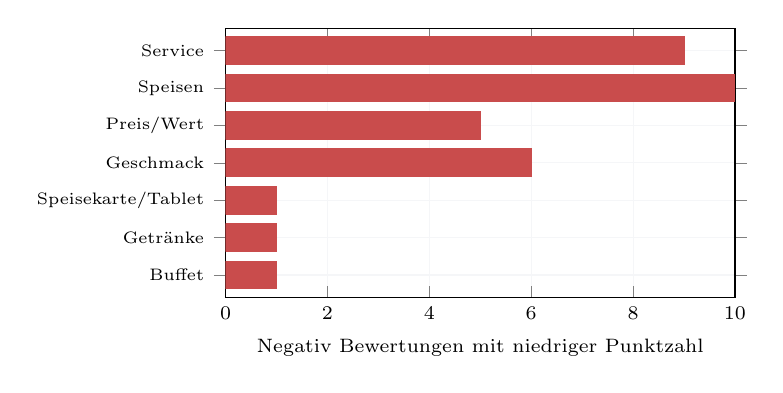
\begin{tikzpicture}\begin{axis}[xbar,width=8.05cm,height=5.0cm,xmin=0,xmax=10,symbolic y coords={Buffet,Drinks,Menu,Taste,Price,Food,Service},ytick=data,yticklabels={Buffet,Getränke,Speisekarte/Tablet,Geschmack,Preis/Wert,Speisen,Service},y tick label style={font=\fontsize{6.2}{7.2}\selectfont},xtick={0,2,4,6,8,10},xticklabel style={font=\scriptsize},xlabel={Negativ Bewertungen mit niedriger Punktzahl},xlabel style={font=\scriptsize},grid=major,grid style={LightGray}]\addplot[fill=Red,draw=Red] coordinates {(\LowBuffetCount,Buffet) (\LowDrinksCount,Drinks) (\LowMenuCount,Menu) (\LowTasteCount,Taste) (\LowPriceCount,Price) (\LowFoodCount,Food) (\LowServiceCount,Service)};\end{axis}\end{tikzpicture}\column{0.38\textwidth}{\fontsize{7.3}{8.7}\selectfont Service \LowServiceCount\ (\LowServicePct\%, \LowServiceEvidence); Speisen \LowFoodCount\ (\LowFoodPct\%, \LowFoodEvidence); Preis/Wert \LowPriceCount\ (\LowPricePct\%, \LowPriceEvidence); Geschmack \LowTasteCount\ (\LowTastePct\%, \LowTasteEvidence); Speisekarte/Tablet \LowMenuCount; Getränke \LowDrinksCount; Buffet \LowBuffetCount.\par\vspace{0.14cm}\textbf{Einordnung:} Service ist der klarste wiederkehrende operative Bereich. Speisen und Preis-Leistung treten wiederholt, aber seltener auf. Einmalige Themen bleiben Prüfsignale.}
  \end{columns}\vfill\backbutton{m-badpatterns}{Zurück zu Muster niedriger Bewertungen}
\end{frame}

\begin{frame}{Anhang D2 - Gemeinsame Problemnennungen und jüngste Verschiebung}
  \hypertarget{a-bad-cooccurrence}{}\appendixhead{D2 - Gemeinsame Nennungen und Zeitpunkt}
  \begin{columns}[T,onlytextwidth]\column{0.52\textwidth}\smallcapslabel{Repeated combinations}\par\vspace{0.09cm}\evidenceitem{\LowPairOneName}{\LowPairOneCount\ Fälle | \LowPairOneShare\%}{\badge{PaleGold}{REPEATED}}\evidenceitem{\LowPairTwoName}{\LowPairTwoCount\ Fälle | \LowPairTwoShare\%}{\badge{PaleGold}{REPEATED}}\vspace{0.12cm}{\fontsize{7.2}{8.6}\selectfont Alle anderen Kombinationen treten einmal auf. Gemeinsame Nennungen helfen bei der Prüfung, beweisen aber keine Ursache. Tages-, Uhrzeit- und Schichtdaten sind nicht verfügbar.}\column{0.44\textwidth}\smallcapslabel{Letzte 90 Tage gegenüber historisch}\par\vspace{0.08cm}{\fontsize{7.4}{8.8}\selectfont Speisen: \LowRecentFoodHistorical\ $\rightarrow$ \LowRecentFoodRecent\ (+\LowRecentFoodChange\ pp; aktuelle Evidenz nach Stützung gewichtet)\\Geschmack: \LowRecentTasteHistorical\ $\rightarrow$ \LowRecentTasteRecent\ (+\LowRecentTasteChange\ pp)\\Service: \LowRecentServiceHistorical\ $\rightarrow$ \LowRecentServiceRecent\ (\LowRecentServiceChange\ pp)\\Preis/Wert: \LowRecentPriceHistorical\ $\rightarrow$ \LowRecentPriceRecent\ (\LowRecentPriceChange\ pp)\par\vspace{0.15cm}\textbf{Zeitraum:} letzte 90 Tage \RecentNinetyStart\ bis \LatestReviewDate; historisch \EarliestReviewDate\ bis \RecentNinetyStart.}
  \end{columns}\vfill\backbutton{m-badpatterns}{Zurück zu Muster niedriger Bewertungen}
\end{frame}

\begin{frame}{Anhang E1 - Negative Serviceevidenz}
  \hypertarget{a-service}{}\appendixhead{E1 - Negative Serviceevidenz}
  \casecard{E01}{31 Aug 2026 | 2 Sterne | letzte 30 Tage | mit Text | Deutsch | Übersetzung ja | Inhaberantwort nein}{Negativ: Speisen, Speisekarte \& Tablet, Parken, Service +2; Positiv: Komfort; Neutral: Buffet, Card Zahlung, Sauberkeit, Getränke +2.}{Artikel: keine erkannt; Buffet ja; Getränke ja; Karte/Tablet ja; Service ja; Preis-Leistung nein.}{Leider müssen wir unsere Bewertung aktualisieren. Die Qualität hat stark abgenommen, bei unserem letzten Besuch wurden weder Salz/Pfeffer noch Öl an den Tisch gebracht und geschmacklich hat ...}{\href{https://www.google.com/maps/Bewertungen/data=!4m8!14m7!1m6!2m5!1sChZDSUhNMG9nS0VKbnJfYUtMMi1yY1ZREAE!2m1!1s0x0:0x27a031a79977995f!3m1!1s2@1:CIHM0ogKEJnr\_aKL2-rcVQ\%7C\%7C?hl=en}{\color{Teal}\fontsize{6.1}{7.2}\selectfont\bfseries Originalbewertung öffnen $\rightarrow$}}
  \casecard{E02}{28 Jul 2026 | 1 Stern | letzte 90 Tage | mit Text | Deutsch | Übersetzung ja | Inhaberantwort nein}{Negativ: Speisen, Speisen Qualität, Meat Qualität, Service +2; Positiv: keine erkannt; Neutral: Getränke.}{Artikel: Gemischte Grillplatte, burger; Buffet nein; Getränke ja; Karte/Tablet nein; Service ja; Preis-Leistung nein.}{Also Burger kam ohne Nachos. Bedienung war überfordert und unfreundlich. Getränke kamen nach der Vorspeise. Teller werden nicht abgeräumt es wird nach Ablage der Gerichte nicht mehr ...}{\href{https://www.google.com/maps/Bewertungen/data=!4m8!14m7!1m6!2m5!1sCi9DQUlRQUNvZENodHljRjlvT2xodWRYUnJabmw1Vld0aFZGVmpNMVF6WlhjMFZVRRAB!2m1!1s0x0:0x27a031a79977995f!3m1!1s2@1:CAIQACodChtycF9oOlhudXRrZnl5VWthVFVjM1QzZXc0VUE\%7C\%7C?hl=en}{\color{Teal}\fontsize{6.1}{7.2}\selectfont\bfseries Originalbewertung öffnen $\rightarrow$}}
  \vfill\backbutton{m-service}{Zurück zu Service}
\end{frame}

\begin{frame}{Anhang E2 - Negative Serviceevidenz}
  \hypertarget{a-service-2}{}\appendixhead{E2 - Negative Serviceevidenz}
  \casecard{E03}{28 Jul 2026 | 1 Stern | letzte 90 Tage | mit Text | Deutsch | Übersetzung ja | Inhaberantwort nein}{Negativ: Speisen, Speisen Qualität, Frische, Service; Positiv: keine erkannt; Neutral: Preis-Leistungs-Verhältnis.}{Artikel: burger; Buffet nein; Getränke nein; Karte/Tablet nein; Service ja; Preis-Leistung ja.}{Wir haben hier u.a. Burger gegessen, der war leider verdorben. Am Nachbartisch das gleiche, aber der Inhaber hat bestritten dass es ein Problem gibt... wir mussten den ...}{\href{https://www.google.com/maps/Bewertungen/data=!4m8!14m7!1m6!2m5!1sCi9DQUlRQUNvZENodHljRjlvT2xWZmFFTndPRzFPVDA1TE5IaEZSV1ZuYW05d1RIYxAB!2m1!1s0x0:0x27a031a79977995f!3m1!1s2@1:CAIQACodChtycF9oOlVfaENwOG1OT05LNHhFRWVnam9wTHc\%7C\%7C?hl=en}{\color{Teal}\fontsize{6.1}{7.2}\selectfont\bfseries Originalbewertung öffnen $\rightarrow$}}
  \casecard{E04}{02 Mai 2026 | 1 Stern | vorherige 90 Tage | mit Text | Englisch | keine Übersetzung erforderlich | Inhaberantwort nein}{Negativ: Speisen, Service, Geschmack; Positiv: keine erkannt; Neutral: keine erkannt.}{Artikel: keine erkannt; Buffet nein; Getränke nein; Karte/Tablet nein; Service ja; Preis-Leistung nein.}{Das Essen schmeckte furchtbar, und das Personal reagierte nicht.}{\href{https://www.google.com/maps/Bewertungen/data=!4m8!14m7!1m6!2m5!1sCi9DQUlRQUNvZENodHljRjlvT2pRd0xWbzNRMk5uUjJaVFMweEhkakZQUzBaamRsRRAB!2m1!1s0x0:0x27a031a79977995f!3m1!1s2@1:CAIQACodChtycF9oOjQwLVo3Q2NnR2ZTS0xHdjFPS0ZjdlE\%7C\%7C?hl=en}{\color{Teal}\fontsize{6.1}{7.2}\selectfont\bfseries Originalbewertung öffnen $\rightarrow$}}
  \vfill\backbutton{m-service}{Zurück zu Service}
\end{frame}

\begin{frame}{Anhang E3 - Negative Serviceevidenz}
  \hypertarget{a-service-3}{}\appendixhead{E3 - Negative Serviceevidenz}
  \casecard{E05}{20 Mär 2026 | 1 Stern | vorherige 90 Tage | mit Text | Deutsch | Übersetzung ja | Inhaberantwort nein}{Negativ: Speisentemperatur, Service; Positiv: Speisen; Neutral: keine erkannt.}{Artikel: keine erkannt; Buffet nein; Getränke nein; Karte/Tablet nein; Service ja; Preis-Leistung nein.}{Am letzten Tag des Ramadan gingen mein Freund und ich essen. Er war schon zweimal dort gewesen, und die Rechnung betrug damals 20 Euro pro Person. Heute ...}{\href{https://www.google.com/maps/Bewertungen/data=!4m8!14m7!1m6!2m5!1sCi9DQUlRQUNvZENodHljRjlvT21KdFp6aFJjRFpRUW1wTE5WZE1VbW94VHpKQlMwRRAB!2m1!1s0x0:0x27a031a79977995f!3m1!1s2@1:CAIQACodChtycF9oOmJtZzhRcDZQQmpLNVdMUmoxTzJBS0E\%7C\%7C?hl=en}{\color{Teal}\fontsize{6.1}{7.2}\selectfont\bfseries Originalbewertung öffnen $\rightarrow$}}
  \casecard{E06}{15 Mär 2026 | 1 Stern | vorherige 90 Tage | mit Text | Arabisch | Übersetzung ja | Inhaberantwort nein}{Negativ: Service; Positiv: keine erkannt; Neutral: keine erkannt.}{Artikel: keine erkannt; Buffet nein; Getränke nein; Karte/Tablet nein; Service ja; Preis-Leistung nein.}{Schlechter Kundenservice.}{\href{https://www.google.com/maps/Bewertungen/data=!4m8!14m7!1m6!2m5!1sCi9DQUlRQUNvZENodHljRjlvT2tORmVrSkNXWGxUTVRVemJYTXhURnBDYUU5NFRsRRAB!2m1!1s0x0:0x27a031a79977995f!3m1!1s2@1:CAIQACodChtycF9oOkNFekJCWXlTMTUzbXMxTFpCaE94TlE\%7C\%7C?hl=en}{\color{Teal}\fontsize{6.1}{7.2}\selectfont\bfseries Originalbewertung öffnen $\rightarrow$}}
  \vfill\backbutton{m-service}{Zurück zu Service}
\end{frame}

\begin{frame}{Anhang E4 - Negative Serviceevidenz}
  \hypertarget{a-service-4}{}\appendixhead{E4 - Negative Serviceevidenz}
  \casecard{E07}{07 Mär 2026 | 2 Sterne | historisch | mit Text | Deutsch | Übersetzung ja | Inhaberantwort nein}{Negativ: Preis-Leistungs-Verhältnis, Service, Wartezeit; Positiv: keine erkannt; Neutral: Speisen.}{Artikel: keine erkannt; Buffet nein; Getränke nein; Karte/Tablet nein; Service ja; Preis-Leistung ja.}{Telefonisch nicht/nie erreichbar. Das Essen ist ganz okay aber dafür zu teuer der Service absolut unfreundlich und wir mussten sehr lange warten.}{\href{https://www.google.com/maps/Bewertungen/data=!4m8!14m7!1m6!2m5!1sCi9DQUlRQUNvZENodHljRjlvT2xSWFUzVkhNMWRDV2pSVWVEVkNlSFUxVVZwWmRtYxAB!2m1!1s0x0:0x27a031a79977995f!3m1!1s2@1:CAIQACodChtycF9oOlRXU3VHM1dCWjRUeDVCeHU1UVpZdmc\%7C\%7C?hl=en}{\color{Teal}\fontsize{6.1}{7.2}\selectfont\bfseries Originalbewertung öffnen $\rightarrow$}}
  \casecard{E08}{21 Jan 2026 | 2 Sterne | historisch | mit Text | Deutsch | Übersetzung ja | Inhaberantwort nein}{Negativ: Preis-Leistungs-Verhältnis, Service; Positiv: Speisen; Neutral: Sauberkeit, Speisenauswahl.}{Artikel: keine erkannt; Buffet nein; Getränke nein; Karte/Tablet nein; Service ja; Preis-Leistung ja.}{Ich war gestern dort mit 6 Personen, um es auszuprobieren. Das Essen war ganz gut und hat mir gefallen, es gab viel Auswahl. Preislich leider viel zu ...}{\href{https://www.google.com/maps/Bewertungen/data=!4m8!14m7!1m6!2m5!1sCi9DQUlRQUNvZENodHljRjlvT21WdmFHSmZUR0YwTjBZMVJtcENlVzFHWkZOaVYwRRAB!2m1!1s0x0:0x27a031a79977995f!3m1!1s2@1:CAIQACodChtycF9oOmVvaGJfTGF0N0Y1RmpCeW1GZFNiV0E\%7C\%7C?hl=en}{\color{Teal}\fontsize{6.1}{7.2}\selectfont\bfseries Originalbewertung öffnen $\rightarrow$}}
  \vfill\backbutton{m-service}{Zurück zu Service}
\end{frame}

\begin{frame}{Anhang E5 - Negative Serviceevidenz}
  \hypertarget{a-service-5}{}\appendixhead{E5 - Negative Serviceevidenz}
  \casecard{E09}{31 Okt 2025 | 1 Stern | historisch | mit Text | Deutsch | Übersetzung ja | Inhaberantwort nein}{Negativ: Service, Freundlichkeit des Personals; Positiv: keine erkannt; Neutral: keine erkannt.}{Artikel: keine erkannt; Buffet nein; Getränke nein; Karte/Tablet nein; Service ja; Preis-Leistung nein.}{Wir sind aus Düsseldorf in das Restaurant gekommen, um es auszuprobieren, aber die Behandlung war sehr schlecht. Wir standen vor der Tür und ein Mitarbeiter kam heraus, ...}{\href{https://www.google.com/maps/Bewertungen/data=!4m8!14m7!1m6!2m5!1sCi9DQUlRQUNvZENodHljRjlvT25NemIyaEhNMGRKYlVOVlMyeDFhbkkyZUhObVUxRRAB!2m1!1s0x0:0x27a031a79977995f!3m1!1s2@1:CAIQACodChtycF9oOnMzb2hHM0dJbUNVS2x1anI2eHNmU1E\%7C\%7C?hl=en}{\color{Teal}\fontsize{6.1}{7.2}\selectfont\bfseries Originalbewertung öffnen $\rightarrow$}}
  \casecard{E10}{11 Aug 2025 | 3 Sterne | historisch | mit Text | Englisch | keine Übersetzung erforderlich | Inhaberantwort nein}{Negativ: Service; Positiv: keine erkannt; Neutral: Speisen.}{Artikel: keine erkannt; Buffet nein; Getränke nein; Karte/Tablet nein; Service ja; Preis-Leistung nein.}{Mir gefiel nicht, dass eine Kellnerin behauptete, mein gewähltes Gericht sei zu klein, und mir zusätzlich einen Salat verkaufte. Das Gericht war ausreichend groß; durch ihre Empfehlung ...}{\href{https://www.google.com/maps/Bewertungen/data=!4m8!14m7!1m6!2m5!1sCi9DQUlRQUNvZENodHljRjlvT25jNVNqSmtXR0ZyYkVJeldHNHdSRk5xVmtaMVdWRRAB!2m1!1s0x0:0x27a031a79977995f!3m1!1s2@1:CAIQACodChtycF9oOnc5SjJkWGFrbEIzWG4wRFNqVkZ1WVE\%7C\%7C?hl=en}{\color{Teal}\fontsize{6.1}{7.2}\selectfont\bfseries Originalbewertung öffnen $\rightarrow$}}
  \vfill\backbutton{m-service}{Zurück zu Service}
\end{frame}

\begin{frame}{Anhang F1 - Negative Evidenz zu Speisen und Geschmack}
  \hypertarget{a-food}{}\appendixhead{F1 - Negative Evidenz zu Speisen und Geschmack}
  \casecard{F01}{31 Aug 2026 | 2 Sterne | letzte 30 Tage | mit Text | Deutsch | Übersetzung ja | Inhaberantwort nein}{Negativ: Speisen, Speisekarte \& Tablet, Parken, Service +2; Positiv: Komfort; Neutral: Buffet, Card Zahlung, Sauberkeit, Getränke +2.}{Artikel: keine erkannt; Buffet ja; Getränke ja; Karte/Tablet ja; Service ja; Preis-Leistung nein.}{Leider müssen wir unsere Bewertung aktualisieren. Die Qualität hat stark abgenommen, bei unserem letzten Besuch wurden weder Salz/Pfeffer noch Öl an den Tisch gebracht und geschmacklich hat ...}{\href{https://www.google.com/maps/Bewertungen/data=!4m8!14m7!1m6!2m5!1sChZDSUhNMG9nS0VKbnJfYUtMMi1yY1ZREAE!2m1!1s0x0:0x27a031a79977995f!3m1!1s2@1:CIHM0ogKEJnr\_aKL2-rcVQ\%7C\%7C?hl=en}{\color{Teal}\fontsize{6.1}{7.2}\selectfont\bfseries Originalbewertung öffnen $\rightarrow$}}
  \casecard{F02}{08 Aug 2026 | 1 Stern | letzte 30 Tage | mit Text | Arabisch | Übersetzung ja | Inhaberantwort nein}{Negativ: Buffet, Speisen, Speisen Qualität, Speisenauswahl +1; Positiv: keine erkannt; Neutral: Buffetauswahl.}{Artikel: Fattoush, kibbeh; Buffet ja; Getränke nein; Karte/Tablet nein; Service nein; Preis-Leistung nein.}{Wir waren zu zweit und bestellten das offene Buffet. Leider waren die Speisen furchtbar und sehr abgestanden. Kein einziges Gericht wirkte frisch. Der Fattoush-Salat war alt und ...}{\href{https://www.google.com/maps/Bewertungen/data=!4m8!14m7!1m6!2m5!1sCi9DQUlRQUNvZENodHljRjlvT21Kc2VrbDZjRmQzWWpCWlJub3hjbXhqU1RoTE5IYxAB!2m1!1s0x0:0x27a031a79977995f!3m1!1s2@1:CAIQACodChtycF9oOmJsekl6cFd3YjBZRnoxcmxjSThLNHc\%7C\%7C?hl=en}{\color{Teal}\fontsize{6.1}{7.2}\selectfont\bfseries Originalbewertung öffnen $\rightarrow$}}
  \vfill\backbutton{m-food}{Zurück zu Speisen/Geschmack}
\end{frame}

\begin{frame}{Anhang F2 - Negative Evidenz zu Speisen und Geschmack}
  \hypertarget{a-food-2}{}\appendixhead{F2 - Negative Evidenz zu Speisen und Geschmack}
  \casecard{F03}{28 Jul 2026 | 1 Stern | letzte 90 Tage | mit Text | Deutsch | Übersetzung ja | Inhaberantwort nein}{Negativ: Speisen, Speisen Qualität, Meat Qualität, Service +2; Positiv: keine erkannt; Neutral: Getränke.}{Artikel: Gemischte Grillplatte, burger; Buffet nein; Getränke ja; Karte/Tablet nein; Service ja; Preis-Leistung nein.}{Also Burger kam ohne Nachos. Bedienung war überfordert und unfreundlich. Getränke kamen nach der Vorspeise. Teller werden nicht abgeräumt es wird nach Ablage der Gerichte nicht mehr ...}{\href{https://www.google.com/maps/Bewertungen/data=!4m8!14m7!1m6!2m5!1sCi9DQUlRQUNvZENodHljRjlvT2xodWRYUnJabmw1Vld0aFZGVmpNMVF6WlhjMFZVRRAB!2m1!1s0x0:0x27a031a79977995f!3m1!1s2@1:CAIQACodChtycF9oOlhudXRrZnl5VWthVFVjM1QzZXc0VUE\%7C\%7C?hl=en}{\color{Teal}\fontsize{6.1}{7.2}\selectfont\bfseries Originalbewertung öffnen $\rightarrow$}}
  \casecard{F04}{28 Jul 2026 | 1 Stern | letzte 90 Tage | mit Text | Deutsch | Übersetzung ja | Inhaberantwort nein}{Negativ: Speisen, Speisen Qualität, Frische, Service; Positiv: keine erkannt; Neutral: Preis-Leistungs-Verhältnis.}{Artikel: burger; Buffet nein; Getränke nein; Karte/Tablet nein; Service ja; Preis-Leistung ja.}{Wir haben hier u.a. Burger gegessen, der war leider verdorben. Am Nachbartisch das gleiche, aber der Inhaber hat bestritten dass es ein Problem gibt... wir mussten den ...}{\href{https://www.google.com/maps/Bewertungen/data=!4m8!14m7!1m6!2m5!1sCi9DQUlRQUNvZENodHljRjlvT2xWZmFFTndPRzFPVDA1TE5IaEZSV1ZuYW05d1RIYxAB!2m1!1s0x0:0x27a031a79977995f!3m1!1s2@1:CAIQACodChtycF9oOlVfaENwOG1OT05LNHhFRWVnam9wTHc\%7C\%7C?hl=en}{\color{Teal}\fontsize{6.1}{7.2}\selectfont\bfseries Originalbewertung öffnen $\rightarrow$}}
  \vfill\backbutton{m-food}{Zurück zu Speisen/Geschmack}
\end{frame}

\begin{frame}{Anhang F3 - Negative Evidenz zu Speisen und Geschmack}
  \hypertarget{a-food-3}{}\appendixhead{F3 - Negative Evidenz zu Speisen und Geschmack}
  \casecard{F05}{26 Jun 2026 | 1 Stern | letzte 90 Tage | mit Text | Deutsch | Übersetzung ja | Inhaberantwort nein}{Negativ: Geschmack; Positiv: Atmosphäre; Neutral: keine erkannt.}{Artikel: Gemischte Grillplatte; Buffet nein; Getränke nein; Karte/Tablet nein; Service nein; Preis-Leistung nein.}{Wir waren zu 4 da und haben Grillteller bestellt, das war leider garnicht gut, es hat uns nicht gefallen es war zu trocken keinen guten Geschmack. Die ...}{\href{https://www.google.com/maps/Bewertungen/data=!4m8!14m7!1m6!2m5!1sCi9DQUlRQUNvZENodHljRjlvT2pKUFJrZERaVXB2ZEZGeWJHbEtabk5GTFZkbk5VRRAB!2m1!1s0x0:0x27a031a79977995f!3m1!1s2@1:CAIQACodChtycF9oOjJPRkdDZUpvdFFybGlKZnNFLVdnNUE\%7C\%7C?hl=en}{\color{Teal}\fontsize{6.1}{7.2}\selectfont\bfseries Originalbewertung öffnen $\rightarrow$}}
  \casecard{F06}{13 Jun 2026 | 1 Stern | letzte 90 Tage | mit Text | Deutsch | Übersetzung ja | Inhaberantwort nein}{Negativ: Speisen, Geschmack; Positiv: keine erkannt; Neutral: keine erkannt.}{Artikel: keine erkannt; Buffet nein; Getränke nein; Karte/Tablet nein; Service nein; Preis-Leistung nein.}{Die Essen gefällt mir nicht.}{\href{https://www.google.com/maps/Bewertungen/data=!4m8!14m7!1m6!2m5!1sCi9DQUlRQUNvZENodHljRjlvT2xrNU5XaFFiblkwUzJFeWFEUTBOMGhaV1ZsTlVGRRAB!2m1!1s0x0:0x27a031a79977995f!3m1!1s2@1:CAIQACodChtycF9oOlk5NWhQbnY0S2EyaDQ0N0hZWVlNUFE\%7C\%7C?hl=en}{\color{Teal}\fontsize{6.1}{7.2}\selectfont\bfseries Originalbewertung öffnen $\rightarrow$}}
  \vfill\backbutton{m-food}{Zurück zu Speisen/Geschmack}
\end{frame}

\begin{frame}{Anhang F4 - Negative Evidenz zu Speisen und Geschmack}
  \hypertarget{a-food-4}{}\appendixhead{F4 - Negative Evidenz zu Speisen und Geschmack}
  \casecard{F07}{08 Mai 2026 | 1 Stern | vorherige 90 Tage | mit Text | Arabisch | Übersetzung ja | Inhaberantwort nein}{Negativ: Speisen; Positiv: keine erkannt; Neutral: keine erkannt.}{Artikel: Shawarma Arabi, shawarma; Buffet nein; Getränke nein; Karte/Tablet nein; Service nein; Preis-Leistung nein.}{Auf der Durchreise durch Bonn kaufte ich leider ein arabisches Shawarma, das überhaupt nicht wie Shawarma schmeckte.}{\href{https://www.google.com/maps/Bewertungen/data=!4m8!14m7!1m6!2m5!1sCi9DQUlRQUNvZENodHljRjlvT25KRWJGZERNRXd4VVRRd2JGTnZNVUZuWm14VWFFRRAB!2m1!1s0x0:0x27a031a79977995f!3m1!1s2@1:CAIQACodChtycF9oOnJEbFdDMEwxUTQwbFNvMUFnZmxUaEE\%7C\%7C?hl=en}{\color{Teal}\fontsize{6.1}{7.2}\selectfont\bfseries Originalbewertung öffnen $\rightarrow$}}
  \casecard{F08}{07 Mai 2026 | 2 Sterne | vorherige 90 Tage | mit Text | Deutsch | Übersetzung ja | Inhaberantwort nein}{Negativ: Speisen, Speisen Qualität, Preis-Leistungs-Verhältnis, Freundlichkeit des Personals +1; Positiv: Service; Neutral: Wartezeit.}{Artikel: shawarma; Buffet nein; Getränke nein; Karte/Tablet nein; Service ja; Preis-Leistung ja.}{Die Shawarma sollte meiner Meinung nach nicht mehr angeboten werden. Sie hat leider nicht gut geschmeckt, viel zu dick geschnitte und war teilweise sogar angebrannt. Ehrlich gesagt ...}{\href{https://www.google.com/maps/Bewertungen/data=!4m8!14m7!1m6!2m5!1sCi9DQUlRQUNvZENodHljRjlvT2xwdlR6RnNkRFp1Tnpsdk1rWkNlbVozY1UxNldGRRAB!2m1!1s0x0:0x27a031a79977995f!3m1!1s2@1:CAIQACodChtycF9oOlpvTzFsdDZuNzlvMkZCemZ3cU16WFE\%7C\%7C?hl=en}{\color{Teal}\fontsize{6.1}{7.2}\selectfont\bfseries Originalbewertung öffnen $\rightarrow$}}
  \vfill\backbutton{m-food}{Zurück zu Speisen/Geschmack}
\end{frame}

\begin{frame}{Anhang F5 - Negative Evidenz zu Speisen und Geschmack}
  \hypertarget{a-food-5}{}\appendixhead{F5 - Negative Evidenz zu Speisen und Geschmack}
  \casecard{F09}{02 Mai 2026 | 1 Stern | vorherige 90 Tage | mit Text | Englisch | keine Übersetzung erforderlich | Inhaberantwort nein}{Negativ: Speisen, Service, Geschmack; Positiv: keine erkannt; Neutral: keine erkannt.}{Artikel: keine erkannt; Buffet nein; Getränke nein; Karte/Tablet nein; Service ja; Preis-Leistung nein.}{Das Essen schmeckte furchtbar, und das Personal reagierte nicht.}{\href{https://www.google.com/maps/Bewertungen/data=!4m8!14m7!1m6!2m5!1sCi9DQUlRQUNvZENodHljRjlvT2pRd0xWbzNRMk5uUjJaVFMweEhkakZQUzBaamRsRRAB!2m1!1s0x0:0x27a031a79977995f!3m1!1s2@1:CAIQACodChtycF9oOjQwLVo3Q2NnR2ZTS0xHdjFPS0ZjdlE\%7C\%7C?hl=en}{\color{Teal}\fontsize{6.1}{7.2}\selectfont\bfseries Originalbewertung öffnen $\rightarrow$}}
  \casecard{F10}{04 Apr 2026 | 1 Stern | vorherige 90 Tage | mit Text | Englisch | keine Übersetzung erforderlich | Inhaberantwort nein}{Negativ: Speisen, Speisen Qualität, Frische, Preis-Leistungs-Verhältnis; Positiv: keine erkannt; Neutral: Buffet.}{Artikel: keine erkannt; Buffet ja; Getränke nein; Karte/Tablet nein; Service nein; Preis-Leistung ja.}{Wir waren hier zum Abendbuffet. Das Essen war nicht gut und abgestanden; mein Mann bekam anschließend eine Lebensmittelvergiftung. Es war eine sehr traurige und schlechte Erfahrung. Auch ...}{\href{https://www.google.com/maps/Bewertungen/data=!4m8!14m7!1m6!2m5!1sCi9DQUlRQUNvZENodHljRjlvT21sS01IRjJWak5mWm1odmREZFRibXR2YVVvNFJGRRAB!2m1!1s0x0:0x27a031a79977995f!3m1!1s2@1:CAIQACodChtycF9oOmlKMHF2VjNfZmhvdDdTbmtvaUo4RFE\%7C\%7C?hl=en}{\color{Teal}\fontsize{6.1}{7.2}\selectfont\bfseries Originalbewertung öffnen $\rightarrow$}}
  \vfill\backbutton{m-food}{Zurück zu Speisen/Geschmack}
\end{frame}

\begin{frame}{Anhang F6 - Negative Evidenz zu Speisen und Geschmack}
  \hypertarget{a-food-6}{}\appendixhead{F6 - Negative Evidenz zu Speisen und Geschmack}
  \casecard{F11}{29 Mär 2026 | 3 Sterne | vorherige 90 Tage | mit Text | Deutsch | Übersetzung ja | Inhaberantwort nein}{Negativ: Buffet, Speisen, Speisen Qualität, Preis-Leistungs-Verhältnis; Positiv: Service, Freundlichkeit des Personals; Neutral: keine erkannt.}{Artikel: keine erkannt; Buffet ja; Getränke nein; Karte/Tablet nein; Service ja; Preis-Leistung ja.}{Die Qualität des Essens bei Buffet ist schlecht, daher ist das Restaurant umsonst teuer. Die Mitarbeiter sind aber freundlich.}{\href{https://www.google.com/maps/Bewertungen/data=!4m8!14m7!1m6!2m5!1sCi9DQUlRQUNvZENodHljRjlvT20xeWFqY3piMVV4Ym1jeFRGRkVWbXhOU3kxNmEzYxAB!2m1!1s0x0:0x27a031a79977995f!3m1!1s2@1:CAIQACodChtycF9oOm1yajczb1UxbmcxTFFEVmxNSy16a3c\%7C\%7C?hl=en}{\color{Teal}\fontsize{6.1}{7.2}\selectfont\bfseries Originalbewertung öffnen $\rightarrow$}}
  \casecard{F12}{20 Mär 2026 | 1 Stern | vorherige 90 Tage | mit Text | Deutsch | Übersetzung ja | Inhaberantwort nein}{Negativ: Speisentemperatur, Service; Positiv: Speisen; Neutral: keine erkannt.}{Artikel: keine erkannt; Buffet nein; Getränke nein; Karte/Tablet nein; Service ja; Preis-Leistung nein.}{Am letzten Tag des Ramadan gingen mein Freund und ich essen. Er war schon zweimal dort gewesen, und die Rechnung betrug damals 20 Euro pro Person. Heute ...}{\href{https://www.google.com/maps/Bewertungen/data=!4m8!14m7!1m6!2m5!1sCi9DQUlRQUNvZENodHljRjlvT21KdFp6aFJjRFpRUW1wTE5WZE1VbW94VHpKQlMwRRAB!2m1!1s0x0:0x27a031a79977995f!3m1!1s2@1:CAIQACodChtycF9oOmJtZzhRcDZQQmpLNVdMUmoxTzJBS0E\%7C\%7C?hl=en}{\color{Teal}\fontsize{6.1}{7.2}\selectfont\bfseries Originalbewertung öffnen $\rightarrow$}}
  \vfill\backbutton{m-food}{Zurück zu Speisen/Geschmack}
\end{frame}

\begin{frame}{Anhang F7 - Negative Evidenz zu Speisen und Geschmack}
  \hypertarget{a-food-7}{}\appendixhead{F7 - Negative Evidenz zu Speisen und Geschmack}
  \casecard{F13}{14 Feb 2026 | 1 Stern | historisch | mit Text | Deutsch | Übersetzung ja | Inhaberantwort nein}{Negativ: Buffetnachfüllung, Speisen, Speisen Qualität; Positiv: keine erkannt; Neutral: keine erkannt.}{Artikel: keine erkannt; Buffet nein; Getränke nein; Karte/Tablet nein; Service nein; Preis-Leistung nein.}{Das Essen ist so eklig 5 mal Haare im essen gesehen Essen ist immer leer wird kaum aufgefüllt einfach niewieder}{\href{https://www.google.com/maps/Bewertungen/data=!4m8!14m7!1m6!2m5!1sCi9DQUlRQUNvZENodHljRjlvT2paRFZGY3paMGREUkVoRU1qVjBTME5uVWtnd1oyYxAB!2m1!1s0x0:0x27a031a79977995f!3m1!1s2@1:CAIQACodChtycF9oOjZDVFczZ0dDREhEMjV0S0NnUkgwZ2c\%7C\%7C?hl=en}{\color{Teal}\fontsize{6.1}{7.2}\selectfont\bfseries Originalbewertung öffnen $\rightarrow$}}
  \vfill\backbutton{m-food}{Zurück zu Speisen/Geschmack}
\end{frame}

\begin{frame}{Anhang G1 - Negative/neutrale Evidenz zu Bar und Getränken}
  \hypertarget{a-bar}{}\appendixhead{G1 - Negative/neutrale Evidenz zu Bar und Getränken}
  \casecard{G01}{31 Aug 2026 | 2 Sterne | letzte 30 Tage | mit Text | Deutsch | Übersetzung ja | Inhaberantwort nein}{Negativ: Speisen, Speisekarte \& Tablet, Parken, Service +2; Positiv: Komfort; Neutral: Buffet, Card Zahlung, Sauberkeit, Getränke +2.}{Artikel: keine erkannt; Buffet ja; Getränke ja; Karte/Tablet ja; Service ja; Preis-Leistung nein.}{Leider müssen wir unsere Bewertung aktualisieren. Die Qualität hat stark abgenommen, bei unserem letzten Besuch wurden weder Salz/Pfeffer noch Öl an den Tisch gebracht und geschmacklich hat ...}{\href{https://www.google.com/maps/Bewertungen/data=!4m8!14m7!1m6!2m5!1sChZDSUhNMG9nS0VKbnJfYUtMMi1yY1ZREAE!2m1!1s0x0:0x27a031a79977995f!3m1!1s2@1:CIHM0ogKEJnr\_aKL2-rcVQ\%7C\%7C?hl=en}{\color{Teal}\fontsize{6.1}{7.2}\selectfont\bfseries Originalbewertung öffnen $\rightarrow$}}
  \casecard{G02}{12 Aug 2026 | 2 Sterne | letzte 30 Tage | mit Text | Deutsch | Übersetzung ja | Inhaberantwort nein}{Negativ: Getränke, Wartezeit; Positiv: Geschmack; Neutral: Speisen, Service.}{Artikel: keine erkannt; Buffet nein; Getränke ja; Karte/Tablet nein; Service ja; Preis-Leistung nein.}{Essen kam nach über einer Stunde immnoch nicht war trozdem lecker. Der Service war okay haben aber das falsche Getränk bekommen.}{\href{https://www.google.com/maps/Bewertungen/data=!4m8!14m7!1m6!2m5!1sCi9DQUlRQUNvZENodHljRjlvT205UGNsZEdkbTlXUW10aVJUZGpjak5CY1hSQmFWRRAB!2m1!1s0x0:0x27a031a79977995f!3m1!1s2@1:CAIQACodChtycF9oOm9PcldGdm9WQmtiRTdjcjNBcXRBaVE\%7C\%7C?hl=en}{\color{Teal}\fontsize{6.1}{7.2}\selectfont\bfseries Originalbewertung öffnen $\rightarrow$}}
  \vfill\backbutton{m-bar}{Zurück zu Bar/Getränken}
\end{frame}

\begin{frame}{Anhang G2 - Negative/neutrale Evidenz zu Bar und Getränken}
  \hypertarget{a-bar-2}{}\appendixhead{G2 - Negative/neutrale Evidenz zu Bar und Getränken}
  \casecard{G03}{28 Jul 2026 | 1 Stern | letzte 90 Tage | mit Text | Deutsch | Übersetzung ja | Inhaberantwort nein}{Negativ: Speisen, Speisen Qualität, Meat Qualität, Service +2; Positiv: keine erkannt; Neutral: Getränke.}{Artikel: Gemischte Grillplatte, burger; Buffet nein; Getränke ja; Karte/Tablet nein; Service ja; Preis-Leistung nein.}{Also Burger kam ohne Nachos. Bedienung war überfordert und unfreundlich. Getränke kamen nach der Vorspeise. Teller werden nicht abgeräumt es wird nach Ablage der Gerichte nicht mehr ...}{\href{https://www.google.com/maps/Bewertungen/data=!4m8!14m7!1m6!2m5!1sCi9DQUlRQUNvZENodHljRjlvT2xodWRYUnJabmw1Vld0aFZGVmpNMVF6WlhjMFZVRRAB!2m1!1s0x0:0x27a031a79977995f!3m1!1s2@1:CAIQACodChtycF9oOlhudXRrZnl5VWthVFVjM1QzZXc0VUE\%7C\%7C?hl=en}{\color{Teal}\fontsize{6.1}{7.2}\selectfont\bfseries Originalbewertung öffnen $\rightarrow$}}
  \casecard{G04}{22 Mai 2026 | 3 Sterne | vorherige 90 Tage | mit Text | Deutsch | Übersetzung ja | Inhaberantwort nein}{Negativ: Getränke, Preis-Leistungs-Verhältnis, Aufmerksamkeit des Personals; Positiv: Speisen, Geschmack; Neutral: Speisen Qualität, Meat Qualität, Service, Kommunikation des Personals.}{Artikel: Gemischte Grillplatte; Buffet nein; Getränke ja; Karte/Tablet nein; Service ja; Preis-Leistung ja.}{Wir sind letztes Jahr aufgrund des leckeren Essens und den angemessen Preisen zu Stammgästen geworden und waren oft da. Da wir gerne im Freien Sitzen, waren wir ...}{\href{https://www.google.com/maps/Bewertungen/data=!4m8!14m7!1m6!2m5!1sCi9DQUlRQUNvZENodHljRjlvT21kU1owRlJZbEJ3V21wUVkzcFlYM0Z2TlRoTk5XYxAB!2m1!1s0x0:0x27a031a79977995f!3m1!1s2@1:CAIQACodChtycF9oOmdSZ0FRYlBwWmpQY3pYX3FvNThNNWc\%7C\%7C?hl=en}{\color{Teal}\fontsize{6.1}{7.2}\selectfont\bfseries Originalbewertung öffnen $\rightarrow$}}
  \vfill\backbutton{m-bar}{Zurück zu Bar/Getränken}
\end{frame}

\begin{frame}{Anhang H1 - Negative/neutrale Buffetevidenz}
  \hypertarget{a-buffet}{}\appendixhead{H1 - Negative/neutrale Buffetevidenz}
  \casecard{H01}{31 Aug 2026 | 2 Sterne | letzte 30 Tage | mit Text | Deutsch | Übersetzung ja | Inhaberantwort nein}{Negativ: Speisen, Speisekarte \& Tablet, Parken, Service +2; Positiv: Komfort; Neutral: Buffet, Card Zahlung, Sauberkeit, Getränke +2.}{Artikel: keine erkannt; Buffet ja; Getränke ja; Karte/Tablet ja; Service ja; Preis-Leistung nein.}{Leider müssen wir unsere Bewertung aktualisieren. Die Qualität hat stark abgenommen, bei unserem letzten Besuch wurden weder Salz/Pfeffer noch Öl an den Tisch gebracht und geschmacklich hat ...}{\href{https://www.google.com/maps/Bewertungen/data=!4m8!14m7!1m6!2m5!1sChZDSUhNMG9nS0VKbnJfYUtMMi1yY1ZREAE!2m1!1s0x0:0x27a031a79977995f!3m1!1s2@1:CIHM0ogKEJnr\_aKL2-rcVQ\%7C\%7C?hl=en}{\color{Teal}\fontsize{6.1}{7.2}\selectfont\bfseries Originalbewertung öffnen $\rightarrow$}}
  \casecard{H02}{08 Aug 2026 | 1 Stern | letzte 30 Tage | mit Text | Arabisch | Übersetzung ja | Inhaberantwort nein}{Negativ: Buffet, Speisen, Speisen Qualität, Speisenauswahl +1; Positiv: keine erkannt; Neutral: Buffetauswahl.}{Artikel: Fattoush, kibbeh; Buffet ja; Getränke nein; Karte/Tablet nein; Service nein; Preis-Leistung nein.}{Wir waren zu zweit und bestellten das offene Buffet. Leider waren die Speisen furchtbar und sehr abgestanden. Kein einziges Gericht wirkte frisch. Der Fattoush-Salat war alt und ...}{\href{https://www.google.com/maps/Bewertungen/data=!4m8!14m7!1m6!2m5!1sCi9DQUlRQUNvZENodHljRjlvT21Kc2VrbDZjRmQzWWpCWlJub3hjbXhqU1RoTE5IYxAB!2m1!1s0x0:0x27a031a79977995f!3m1!1s2@1:CAIQACodChtycF9oOmJsekl6cFd3YjBZRnoxcmxjSThLNHc\%7C\%7C?hl=en}{\color{Teal}\fontsize{6.1}{7.2}\selectfont\bfseries Originalbewertung öffnen $\rightarrow$}}
  \vfill\backbutton{m-buffet}{Zurück zu Buffet}
\end{frame}

\begin{frame}{Anhang H2 - Negative/neutrale Buffetevidenz}
  \hypertarget{a-buffet-2}{}\appendixhead{H2 - Negative/neutrale Buffetevidenz}
  \casecard{H03}{16 Mai 2026 | 5 Sterne | vorherige 90 Tage | mit Text | Arabisch | Übersetzung ja | Inhaberantwort nein}{Negativ: keine erkannt; Positiv: Speisen, Geschmack; Neutral: Authentizität, Buffet, Portionsgröße, Preis-Leistungs-Verhältnis +1.}{Artikel: keine erkannt; Buffet ja; Getränke nein; Karte/Tablet nein; Service ja; Preis-Leistung ja.}{Sehr köstliche Speisen, zubereitet von erfahrenen Köchen mit Leidenschaft und Kreativität. Jedes Gericht folgt traditionellen Rezepten und wird mit großer Sorgfalt zubereitet. Entscheidend sind nicht nur große ...}{\href{https://www.google.com/maps/Bewertungen/data=!4m8!14m7!1m6!2m5!1sCi9DQUlRQUNvZENodHljRjlvT2sxR1NEZE9YMGhTUWxweVFYaFpTMFpXVVhOZmFGRRAB!2m1!1s0x0:0x27a031a79977995f!3m1!1s2@1:CAIQACodChtycF9oOk1GSDdOX0hSQlpyQXhZS0ZWUXNfaFE\%7C\%7C?hl=en}{\color{Teal}\fontsize{6.1}{7.2}\selectfont\bfseries Originalbewertung öffnen $\rightarrow$}}
  \casecard{H04}{04 Apr 2026 | 1 Stern | vorherige 90 Tage | mit Text | Englisch | keine Übersetzung erforderlich | Inhaberantwort nein}{Negativ: Speisen, Speisen Qualität, Frische, Preis-Leistungs-Verhältnis; Positiv: keine erkannt; Neutral: Buffet.}{Artikel: keine erkannt; Buffet ja; Getränke nein; Karte/Tablet nein; Service nein; Preis-Leistung ja.}{Wir waren hier zum Abendbuffet. Das Essen war nicht gut und abgestanden; mein Mann bekam anschließend eine Lebensmittelvergiftung. Es war eine sehr traurige und schlechte Erfahrung. Auch ...}{\href{https://www.google.com/maps/Bewertungen/data=!4m8!14m7!1m6!2m5!1sCi9DQUlRQUNvZENodHljRjlvT21sS01IRjJWak5mWm1odmREZFRibXR2YVVvNFJGRRAB!2m1!1s0x0:0x27a031a79977995f!3m1!1s2@1:CAIQACodChtycF9oOmlKMHF2VjNfZmhvdDdTbmtvaUo4RFE\%7C\%7C?hl=en}{\color{Teal}\fontsize{6.1}{7.2}\selectfont\bfseries Originalbewertung öffnen $\rightarrow$}}
  \vfill\backbutton{m-buffet}{Zurück zu Buffet}
\end{frame}

\begin{frame}{Anhang H3 - Negative/neutrale Buffetevidenz}
  \hypertarget{a-buffet-3}{}\appendixhead{H3 - Negative/neutrale Buffetevidenz}
  \casecard{H05}{29 Mär 2026 | 3 Sterne | vorherige 90 Tage | mit Text | Deutsch | Übersetzung ja | Inhaberantwort nein}{Negativ: Buffet, Speisen, Speisen Qualität, Preis-Leistungs-Verhältnis; Positiv: Service, Freundlichkeit des Personals; Neutral: keine erkannt.}{Artikel: keine erkannt; Buffet ja; Getränke nein; Karte/Tablet nein; Service ja; Preis-Leistung ja.}{Die Qualität des Essens bei Buffet ist schlecht, daher ist das Restaurant umsonst teuer. Die Mitarbeiter sind aber freundlich.}{\href{https://www.google.com/maps/Bewertungen/data=!4m8!14m7!1m6!2m5!1sCi9DQUlRQUNvZENodHljRjlvT20xeWFqY3piMVV4Ym1jeFRGRkVWbXhOU3kxNmEzYxAB!2m1!1s0x0:0x27a031a79977995f!3m1!1s2@1:CAIQACodChtycF9oOm1yajczb1UxbmcxTFFEVmxNSy16a3c\%7C\%7C?hl=en}{\color{Teal}\fontsize{6.1}{7.2}\selectfont\bfseries Originalbewertung öffnen $\rightarrow$}}
  \casecard{H06}{22 Mär 2026 | 4 Sterne | vorherige 90 Tage | mit Text | Deutsch | Übersetzung ja | Inhaberantwort nein}{Negativ: Buffet; Positiv: Speisen, Speisenauswahl, Speisekarte \& Tablet, Geschmack; Neutral: keine erkannt.}{Artikel: keine erkannt; Buffet ja; Getränke nein; Karte/Tablet ja; Service nein; Preis-Leistung nein.}{A la carte sehr zu empfehlen. Mittags/Abendbuffet nicht zu empfehlen. Keine große Auswahl und geschmacklich auch nichts Besonderes. Haben uns beim letzten Besuch für das Buffet entschieden ...}{\href{https://www.google.com/maps/Bewertungen/data=!4m8!14m7!1m6!2m5!1sCi9DQUlRQUNvZENodHljRjlvT2sxMGQwNUtjMlJFVFdoQmJFSkNlRTVTVjNCWWEwRRAB!2m1!1s0x0:0x27a031a79977995f!3m1!1s2@1:CAIQACodChtycF9oOk10d05Kc2RETWhBbEJCeE5SV3BYa0E\%7C\%7C?hl=en}{\color{Teal}\fontsize{6.1}{7.2}\selectfont\bfseries Originalbewertung öffnen $\rightarrow$}}
  \vfill\backbutton{m-buffet}{Zurück zu Buffet}
\end{frame}

\begin{frame}{Anhang H4 - Negative/neutrale Buffetevidenz}
  \hypertarget{a-buffet-4}{}\appendixhead{H4 - Negative/neutrale Buffetevidenz}
  \casecard{H07}{26 Feb 2026 | 3 Sterne | historisch | mit Text | Deutsch | Übersetzung ja | Inhaberantwort nein}{Negativ: Reservierungen; Positiv: Atmosphäre, Anrichtung, Service; Neutral: Buffet, Speisen, Speisentemperatur.}{Artikel: keine erkannt; Buffet ja; Getränke nein; Karte/Tablet nein; Service ja; Preis-Leistung nein.}{Ehrlich gesagt bin ich enttäuscht.. Nach so vielen Empfehlungen wollte ich dieses Restaurant auch mal ausprobieren Ich war im Ramadan da zum Ramadan Buffet. Ich habe zuvor ...}{\href{https://www.google.com/maps/Bewertungen/data=!4m8!14m7!1m6!2m5!1sCi9DQUlRQUNvZENodHljRjlvT2xwM1pHNUpZVXg0TkRka2NFaEhhbVIzTFRKR1NsRRAB!2m1!1s0x0:0x27a031a79977995f!3m1!1s2@1:CAIQACodChtycF9oOlp3ZG5JYUx4NDdkcEhHamR3LTJGSlE\%7C\%7C?hl=en}{\color{Teal}\fontsize{6.1}{7.2}\selectfont\bfseries Originalbewertung öffnen $\rightarrow$}}
  \casecard{H08}{15 Feb 2026 | 4 Sterne | historisch | mit Text | Deutsch | Übersetzung ja | Inhaberantwort nein}{Negativ: keine erkannt; Positiv: Atmosphäre, Authentizität, Komfort, Speisen +5; Neutral: Buffet, Speisenauswahl.}{Artikel: keine erkannt; Buffet ja; Getränke nein; Karte/Tablet nein; Service ja; Preis-Leistung ja.}{4,3 Sterne würde ich geben. Waren zum Buffet essen im Restaurant (über ein Angebotspreis) An dem Tag gab es eine kleinere Auswahl, die aber trotzdem groß genug ...}{\href{https://www.google.com/maps/Bewertungen/data=!4m8!14m7!1m6!2m5!1sCi9DQUlRQUNvZENodHljRjlvT2poSGIwSmlRalEzVWpCVk0wTlpSbFpxUVVWSU9XYxAB!2m1!1s0x0:0x27a031a79977995f!3m1!1s2@1:CAIQACodChtycF9oOjhHb0JiQjQ3UjBVM0NZRlZqQUVIOWc\%7C\%7C?hl=en}{\color{Teal}\fontsize{6.1}{7.2}\selectfont\bfseries Originalbewertung öffnen $\rightarrow$}}
  \vfill\backbutton{m-buffet}{Zurück zu Buffet}
\end{frame}

\begin{frame}{Anhang H5 - Negative/neutrale Buffetevidenz}
  \hypertarget{a-buffet-5}{}\appendixhead{H5 - Negative/neutrale Buffetevidenz}
  \casecard{H09}{14 Feb 2026 | 1 Stern | historisch | mit Text | Deutsch | Übersetzung ja | Inhaberantwort nein}{Negativ: Gastfreundschaft, Preis-Leistungs-Verhältnis, Wartezeit; Positiv: keine erkannt; Neutral: Buffet, Family \& Groups, Speisen, Speisenauswahl.}{Artikel: keine erkannt; Buffet ja; Getränke nein; Karte/Tablet nein; Service nein; Preis-Leistung ja.}{über Groupon haben wir einen Gutschein für Ihr Buffet erworben. Dort wurde ein regulärer Preis von 35 € angegeben, wodurch wir ein entsprechend umfangreiches und vielfältiges Buffet ...}{\href{https://www.google.com/maps/Bewertungen/data=!4m8!14m7!1m6!2m5!1sCi9DQUlRQUNvZENodHljRjlvT2tOeVVEQkplRUZsVkVSNFlqaHJlbUZLVEVGSllXYxAB!2m1!1s0x0:0x27a031a79977995f!3m1!1s2@1:CAIQACodChtycF9oOkNyUDBJeEFlVER4YjhremFKTEFJYWc\%7C\%7C?hl=en}{\color{Teal}\fontsize{6.1}{7.2}\selectfont\bfseries Originalbewertung öffnen $\rightarrow$}}
  \casecard{H10}{24 Jan 2026 | 3 Sterne | historisch | mit Text | Deutsch | Übersetzung ja | Inhaberantwort nein}{Negativ: keine erkannt; Positiv: keine erkannt; Neutral: Buffet, Vegetarian \& Vegan.}{Artikel: keine erkannt; Buffet ja; Getränke nein; Karte/Tablet nein; Service nein; Preis-Leistung nein.}{Das Konzept wurde geändert und es gab nur Buffet. Leider waren keine vegetarischen Hauptgerichte dabei.}{\href{https://www.google.com/maps/Bewertungen/data=!4m8!14m7!1m6!2m5!1sCi9DQUlRQUNvZENodHljRjlvT25jdE5WVmZTRk5OVm5sTE5HVmZiSEpaYVdKcWVWRRAB!2m1!1s0x0:0x27a031a79977995f!3m1!1s2@1:CAIQACodChtycF9oOnctNVVfSFNNVnlLNGVfbHJZaWJqeVE\%7C\%7C?hl=en}{\color{Teal}\fontsize{6.1}{7.2}\selectfont\bfseries Originalbewertung öffnen $\rightarrow$}}
  \vfill\backbutton{m-buffet}{Zurück zu Buffet}
\end{frame}

\begin{frame}{Anhang H6 - Negative/neutrale Buffetevidenz}
  \hypertarget{a-buffet-6}{}\appendixhead{H6 - Negative/neutrale Buffetevidenz}
  \casecard{H11}{03 Aug 2025 | 5 Sterne | historisch | mit Text | Deutsch | Übersetzung ja | Inhaberantwort nein}{Negativ: keine erkannt; Positiv: Atmosphäre, Speisenauswahl, Preis-Leistungs-Verhältnis, Service; Neutral: Buffet.}{Artikel: keine erkannt; Buffet ja; Getränke nein; Karte/Tablet nein; Service ja; Preis-Leistung ja.}{Wir waren heute am Sonntag zum Frühstückbüfett da, hat uns sehr gut gefallen. Sehr gutes Frühstück, Reichlich und viel Auswahl. Personal ist sehr nett, gute Ambiente, Preiswert ...}{\href{https://www.google.com/maps/Bewertungen/data=!4m8!14m7!1m6!2m5!1sCi9DQUlRQUNvZENodHljRjlvT2todVZrOWxSRTUxTlV4UmNsWTFZMHgzTm5OUFRXYxAB!2m1!1s0x0:0x27a031a79977995f!3m1!1s2@1:CAIQACodChtycF9oOkhuVk9lRE51NUxRclY1Y0x3NnNPTWc\%7C\%7C?hl=en}{\color{Teal}\fontsize{6.1}{7.2}\selectfont\bfseries Originalbewertung öffnen $\rightarrow$}}
  \vfill\backbutton{m-buffet}{Zurück zu Buffet}
\end{frame}

\begin{frame}{Anhang I1 - Beschwerdeevidenz zu Speisekarte und Tablet}
  \hypertarget{a-menu}{}\appendixhead{I1 - Beschwerdeevidenz zu Speisekarte und Tablet}
  \casecard{I01}{31 Aug 2026 | 2 Sterne | letzte 30 Tage | mit Text | Deutsch | Übersetzung ja | Inhaberantwort nein}{Negativ: Speisen, Speisekarte \& Tablet, Parken, Service +2; Positiv: Komfort; Neutral: Buffet, Card Zahlung, Sauberkeit, Getränke +2.}{Artikel: keine erkannt; Buffet ja; Getränke ja; Karte/Tablet ja; Service ja; Preis-Leistung nein.}{Leider müssen wir unsere Bewertung aktualisieren. Die Qualität hat stark abgenommen, bei unserem letzten Besuch wurden weder Salz/Pfeffer noch Öl an den Tisch gebracht und geschmacklich hat ...}{\href{https://www.google.com/maps/Bewertungen/data=!4m8!14m7!1m6!2m5!1sChZDSUhNMG9nS0VKbnJfYUtMMi1yY1ZREAE!2m1!1s0x0:0x27a031a79977995f!3m1!1s2@1:CIHM0ogKEJnr\_aKL2-rcVQ\%7C\%7C?hl=en}{\color{Teal}\fontsize{6.1}{7.2}\selectfont\bfseries Originalbewertung öffnen $\rightarrow$}}
  \casecard{I02}{29 Sep 2025 | 5 Sterne | historisch | mit Text | Deutsch | Übersetzung ja | Inhaberantwort nein}{Negativ: keine erkannt; Positiv: keine erkannt; Neutral: Speisen, Speisekarte \& Tablet.}{Artikel: keine erkannt; Buffet nein; Getränke nein; Karte/Tablet ja; Service nein; Preis-Leistung nein.}{Ich war erst skeptisch als ich die karte sah waren sowohl syrische Gerichte wie auch internationale zu finden, die Speisen waren klasse abgeschmeckt, mit liebe zubereitet und ...}{\href{https://www.google.com/maps/Bewertungen/data=!4m8!14m7!1m6!2m5!1sCi9DQUlRQUNvZENodHljRjlvT2xJMWJGWlJNM0pHY3pselNrNVdjVzVwZFhobFVHYxAB!2m1!1s0x0:0x27a031a79977995f!3m1!1s2@1:CAIQACodChtycF9oOlI1bFZRM3JGczlzSk5WcW5pdXhlUGc\%7C\%7C?hl=en}{\color{Teal}\fontsize{6.1}{7.2}\selectfont\bfseries Originalbewertung öffnen $\rightarrow$}}
  \vfill\backbutton{m-menu}{Zurück zu Speisekarte \& Bestellung}
\end{frame}

\begin{frame}{Anhang I2 - Beschwerdeevidenz zu Speisekarte und Tablet}
  \hypertarget{a-menu-2}{}\appendixhead{I2 - Beschwerdeevidenz zu Speisekarte und Tablet}
  \casecard{I03}{27 Jan 2025 | 5 Sterne | historisch | mit Text | Deutsch | Übersetzung ja | Inhaberantwort ja}{Negativ: keine erkannt; Positiv: Speisen, Speisen Qualität, Speisenauswahl, Frische +5; Neutral: Atmosphäre, Speisekarte \& Tablet, Parken.}{Artikel: keine erkannt; Buffet nein; Getränke nein; Karte/Tablet ja; Service ja; Preis-Leistung nein.}{Das Restaurant und die Ambiente dort sind sehr einladend. Absolut empfehlenswert! Die Qualität, die Zutaten, und die Zubereitung sind einfach top und unglaublich lecker. Es gibt dort ...}{\href{https://www.google.com/maps/Bewertungen/data=!4m8!14m7!1m6!2m5!1sChZDSUhNMG9nS0VJQ0FnSURfaC1lV1hnEAE!2m1!1s0x0:0x27a031a79977995f!3m1!1s2@1:CIHM0ogKEICAgID\_h-eWXg\%7C\%7C?hl=en}{\color{Teal}\fontsize{6.1}{7.2}\selectfont\bfseries Originalbewertung öffnen $\rightarrow$}}
  \vfill\backbutton{m-menu}{Zurück zu Speisekarte \& Bestellung}
\end{frame}

\begin{frame}{Anhang J1 - Alle erwähnten Gerichte/Artikel}
  \hypertarget{a-dishes}{}\appendixhead{J1 - Gerichte 1-3 von 16}
  \dishcard{Jordanisches Mansaf}{Kategorie: Orientalische Gerichte | Nennungen 6 | positiv 2 | negativ 0 | neutral 4 | Durchschnitt der Gesamtbewertung 5.00 | Evidenz mittel | zuletzt 14 Sep 2025}{Wir hatten Tabbouleh, Fattoush, Sambusek, eine gemischte Vorspeisenplatte, eine Familien-Grillplatte und eine jordanische Mansaf-Platte.}{\href{https://www.google.com/maps/Bewertungen/data=!4m8!14m7!1m6!2m5!1sCi9DQUlRQUNvZENodHljRjlvT2tOMk9FUTJPSHBGT1RCbFRGbFJTelJuYWpCWlJIYxAB!2m1!1s0x0:0x27a031a79977995f!3m1!1s2@1:CAIQACodChtycF9oOkN2OEQ2OHpFOTBlTFlRSzRnajBZRHc\%7C\%7C?hl=en}{\color{Teal}\fontsize{6.1}{7.2}\selectfont\bfseries Originalbewertung öffnen $\rightarrow$}}
  \dishcard{Tabbouleh}{Kategorie: Salate | Nennungen 5 | positiv 3 | negativ 0 | neutral 2 | Durchschnitt der Gesamtbewertung 4.00 | Evidenz mittel | zuletzt 01 Jul 2026}{Das einzige schmackhafte Gericht war Tabbouleh.}{\href{https://www.google.com/maps/Bewertungen/data=!4m8!14m7!1m6!2m5!1sCi9DQUlRQUNvZENodHljRjlvT21sR2VXMVBjMVJ6V1hCbmVUUlNXR2xOWmpKV05sRRAB!2m1!1s0x0:0x27a031a79977995f!3m1!1s2@1:CAIQACodChtycF9oOmlGeW1Pc1RzWXBneTRSWGlNZjJWNlE\%7C\%7C?hl=en}{\color{Teal}\fontsize{6.1}{7.2}\selectfont\bfseries Originalbewertung öffnen $\rightarrow$}}
  \dishcard{Gemischte Grillplatte}{Kategorie: Grillgerichte | Nennungen 4 | positiv 0 | negativ 2 | neutral 2 | Durchschnitt der Gesamtbewertung 2.50 | Evidenz niedrig | zuletzt 28 Jul 2026}{Die Hähnchenflügel auf der gemischten Grillplatte waren verbrannt.}{\href{https://www.google.com/maps/Bewertungen/data=!4m8!14m7!1m6!2m5!1sCi9DQUlRQUNvZENodHljRjlvT2xodWRYUnJabmw1Vld0aFZGVmpNMVF6WlhjMFZVRRAB!2m1!1s0x0:0x27a031a79977995f!3m1!1s2@1:CAIQACodChtycF9oOlhudXRrZnl5VWthVFVjM1QzZXc0VUE\%7C\%7C?hl=en}{\color{Teal}\fontsize{6.1}{7.2}\selectfont\bfseries Originalbewertung öffnen $\rightarrow$}}
  \vfill\backbutton{m-dishes}{Zurück zu erwähnten Gerichten}
\end{frame}

\begin{frame}{Anhang J2 - Alle erwähnten Gerichte/Artikel}
  \hypertarget{a-dishes-2}{}\appendixhead{J2 - Gerichte 4-6 von 16}
  \dishcard{Fattoush}{Kategorie: Salate | Nennungen 3 | positiv 1 | negativ 0 | neutral 2 | Durchschnitt der Gesamtbewertung 3.67 | Evidenz niedrig | zuletzt 08 Aug 2026}{Es gab nur einen Salat, nämlich Fattoush,}{\href{https://www.google.com/maps/Bewertungen/data=!4m8!14m7!1m6!2m5!1sCi9DQUlRQUNvZENodHljRjlvT21Kc2VrbDZjRmQzWWpCWlJub3hjbXhqU1RoTE5IYxAB!2m1!1s0x0:0x27a031a79977995f!3m1!1s2@1:CAIQACodChtycF9oOmJsekl6cFd3YjBZRnoxcmxjSThLNHc\%7C\%7C?hl=en}{\color{Teal}\fontsize{6.1}{7.2}\selectfont\bfseries Originalbewertung öffnen $\rightarrow$}}
  \dishcard{Tee}{Kategorie: Heißgetränke | Nennungen 3 | positiv 2 | negativ 0 | neutral 1 | Durchschnitt der Gesamtbewertung 4.67 | Evidenz niedrig | zuletzt 21 Dez 2025}{15 € pro Person einschließlich Tee boten ein ausgezeichnetes Preis-Leistungs-Verhältnis.}{\href{https://www.google.com/maps/Bewertungen/data=!4m8!14m7!1m6!2m5!1sCi9DQUlRQUNvZENodHljRjlvT2xSRFQzaEJSa3N0Um1oUVdreFVlVGxHVEZONVRVRRAB!2m1!1s0x0:0x27a031a79977995f!3m1!1s2@1:CAIQACodChtycF9oOlRDT3hBRkstRmhQWkxUeTlGTFN5TUE\%7C\%7C?hl=en}{\color{Teal}\fontsize{6.1}{7.2}\selectfont\bfseries Originalbewertung öffnen $\rightarrow$}}
  \dishcard{Linsensuppe}{Kategorie: Suppen | Nennungen 1 | positiv 0 | negativ 0 | neutral 1 | Durchschnitt der Gesamtbewertung 5.00 | Evidenz niedrig | zuletzt 27 Dez 2025}{Die Linsensuppe war eine 10 von 10.}{\href{https://www.google.com/maps/Bewertungen/data=!4m8!14m7!1m6!2m5!1sCi9DQUlRQUNvZENodHljRjlvT21nd2NGQlpibGhST0hoVmRqQnNZV1pKTWt0QlFWRRAB!2m1!1s0x0:0x27a031a79977995f!3m1!1s2@1:CAIQACodChtycF9oOmgwcFBZblhROHhVdjBsYWZJMktBQVE\%7C\%7C?hl=en}{\color{Teal}\fontsize{6.1}{7.2}\selectfont\bfseries Originalbewertung öffnen $\rightarrow$}}
  \vfill\backbutton{m-dishes}{Zurück zu erwähnten Gerichten}
\end{frame}

\begin{frame}{Anhang J3 - Alle erwähnten Gerichte/Artikel}
  \hypertarget{a-dishes-3}{}\appendixhead{J3 - Gerichte 7-9 von 16}
  \dishcard{Mozzarella-Sticks}{Kategorie: Warme Vorspeisen | Nennungen 1 | positiv 0 | negativ 0 | neutral 1 | Durchschnitt der Gesamtbewertung 2.00 | Evidenz niedrig | zuletzt 26 Jan 2025}{Stattdessen werden Mozzarella-Sticks, Pasta und Burger angeboten.}{\href{https://www.google.com/maps/Bewertungen/data=!4m8!14m7!1m6!2m5!1sChZDSUhNMG9nS0VJQ0FnSURfZzhlN1RnEAE!2m1!1s0x0:0x27a031a79977995f!3m1!1s2@1:CIHM0ogKEICAgID\_g8e7Tg\%7C\%7C?hl=en}{\color{Teal}\fontsize{6.1}{7.2}\selectfont\bfseries Originalbewertung öffnen $\rightarrow$}}
  \dishcard{Gemischte Vorspeisenplatte}{Kategorie: Kalte Vorspeisen | Nennungen 1 | positiv 0 | negativ 0 | neutral 1 | Durchschnitt der Gesamtbewertung 5.00 | Evidenz niedrig | zuletzt 14 Sep 2025}{Wir hatten Tabbouleh, Fattoush, Sambusek, eine gemischte Vorspeisenplatte, eine Familien-Grillplatte und eine jordanische Mansaf-Platte.}{\href{https://www.google.com/maps/Bewertungen/data=!4m8!14m7!1m6!2m5!1sCi9DQUlRQUNvZENodHljRjlvT2tOMk9FUTJPSHBGT1RCbFRGbFJTelJuYWpCWlJIYxAB!2m1!1s0x0:0x27a031a79977995f!3m1!1s2@1:CAIQACodChtycF9oOkN2OEQ2OHpFOTBlTFlRSzRnajBZRHc\%7C\%7C?hl=en}{\color{Teal}\fontsize{6.1}{7.2}\selectfont\bfseries Originalbewertung öffnen $\rightarrow$}}
  \dishcard{Hummus}{Kategorie: Kalte Vorspeisen | Nennungen 1 | positiv 1 | negativ 0 | neutral 0 | Durchschnitt der Gesamtbewertung 5.00 | Evidenz niedrig | zuletzt 10 Feb 2025}{Vorspeisen sind mir sehr wichtig, und die hier servierten Vorspeisen - Hummus, Baba Ghanoush, Kebab Neye und Batata ...}{\href{https://www.google.com/maps/Bewertungen/data=!4m8!14m7!1m6!2m5!1sChZDSUhNMG9nS0VJQ0FnTURBaGR1VEZREAE!2m1!1s0x0:0x27a031a79977995f!3m1!1s2@1:CIHM0ogKEICAgMDAhduTFQ\%7C\%7C?hl=en}{\color{Teal}\fontsize{6.1}{7.2}\selectfont\bfseries Originalbewertung öffnen $\rightarrow$}}
  \vfill\backbutton{m-dishes}{Zurück zu erwähnten Gerichten}
\end{frame}

\begin{frame}{Anhang J4 - Alle erwähnten Gerichte/Artikel}
  \hypertarget{a-dishes-4}{}\appendixhead{J4 - Gerichte 10-12 von 16}
  \dishcard{Baba Ghanoush}{Kategorie: Kalte Vorspeisen | Nennungen 1 | positiv 1 | negativ 0 | neutral 0 | Durchschnitt der Gesamtbewertung 5.00 | Evidenz niedrig | zuletzt 10 Feb 2025}{Vorspeisen sind mir sehr wichtig, und die hier servierten Vorspeisen - Hummus, Baba Ghanoush, Kebab Neye und Batata ...}{\href{https://www.google.com/maps/Bewertungen/data=!4m8!14m7!1m6!2m5!1sChZDSUhNMG9nS0VJQ0FnTURBaGR1VEZREAE!2m1!1s0x0:0x27a031a79977995f!3m1!1s2@1:CIHM0ogKEICAgMDAhduTFQ\%7C\%7C?hl=en}{\color{Teal}\fontsize{6.1}{7.2}\selectfont\bfseries Originalbewertung öffnen $\rightarrow$}}
  \dishcard{Shish Taouk}{Kategorie: Grillgerichte | Nennungen 1 | positiv 1 | negativ 0 | neutral 0 | Durchschnitt der Gesamtbewertung 4.00 | Evidenz niedrig | zuletzt 04 Jun 2026}{Mein Favorit war Shish Tawook mit Kartoffeln und einer sehr guten Knoblauchsauce, besser als die anderen Kebabs.}{\href{https://www.google.com/maps/Bewertungen/data=!4m8!14m7!1m6!2m5!1sCi9DQUlRQUNvZENodHljRjlvT2tKUmNESkZNR0pmU0hGM1NXcEdaa1ZOUVZGRWFrRRAB!2m1!1s0x0:0x27a031a79977995f!3m1!1s2@1:CAIQACodChtycF9oOkJRcDJFMGJfSHF3SWpGZkVNQVFEakE\%7C\%7C?hl=en}{\color{Teal}\fontsize{6.1}{7.2}\selectfont\bfseries Originalbewertung öffnen $\rightarrow$}}
  \dishcard{Auberginen-Kebab}{Kategorie: Grillgerichte | Nennungen 1 | positiv 0 | negativ 0 | neutral 1 | Durchschnitt der Gesamtbewertung 5.00 | Evidenz niedrig | zuletzt 23 Mai 2025}{Wir bestellten die Vorspeisenplatte, Mansaf und Auberginen-Kebab.}{\href{https://www.google.com/maps/Bewertungen/data=!4m8!14m7!1m6!2m5!1sChZDSUhNMG9nS0VNS09xdG1ZdWRfNk53EAE!2m1!1s0x0:0x27a031a79977995f!3m1!1s2@1:CIHM0ogKEMKOqtmYud\_6Nw\%7C\%7C?hl=en}{\color{Teal}\fontsize{6.1}{7.2}\selectfont\bfseries Originalbewertung öffnen $\rightarrow$}}
  \vfill\backbutton{m-dishes}{Zurück zu erwähnten Gerichten}
\end{frame}

\begin{frame}{Anhang J5 - Alle erwähnten Gerichte/Artikel}
  \hypertarget{a-dishes-5}{}\appendixhead{J5 - Gerichte 13-15 von 16}
  \dishcard{Lammkoteletts}{Kategorie: Grillgerichte | Nennungen 1 | positiv 1 | negativ 0 | neutral 0 | Durchschnitt der Gesamtbewertung 5.00 | Evidenz niedrig | zuletzt 05 Jul 2025}{Meine Lammkoteletts waren ausgezeichnet und die Vorspeisenauswahl überragend.}{\href{https://www.google.com/maps/Bewertungen/data=!4m8!14m7!1m6!2m5!1sCi9DQUlRQUNvZENodHljRjlvT20xSFFUZGZPRGxMTUVocVZWUlZhV2hHVWtGc2MzYxAB!2m1!1s0x0:0x27a031a79977995f!3m1!1s2@1:CAIQACodChtycF9oOm1HQTdfODlLMEhqVVRVaWhGUkFsc3c\%7C\%7C?hl=en}{\color{Teal}\fontsize{6.1}{7.2}\selectfont\bfseries Originalbewertung öffnen $\rightarrow$}}
  \dishcard{Spicy Chicken}{Kategorie: Burger \& westliche Gerichte | Nennungen 1 | positiv 1 | negativ 0 | neutral 0 | Durchschnitt der Gesamtbewertung 5.00 | Evidenz niedrig | zuletzt 19 Mai 2025}{Zum Hauptgericht muss ich sagen, dass neben den außergewöhnlichen Gerichten mit Kirschsauce zu den Kebab-Bällchen ...}{\href{https://www.google.com/maps/Bewertungen/data=!4m8!14m7!1m6!2m5!1sChZDSUhNMG9nS0VQeXhrUHZHODRLYVRREAE!2m1!1s0x0:0x27a031a79977995f!3m1!1s2@1:CIHM0ogKEPyxkPvG84KaTQ\%7C\%7C?hl=en}{\color{Teal}\fontsize{6.1}{7.2}\selectfont\bfseries Originalbewertung öffnen $\rightarrow$}}
  \dishcard{Shawarma Arabi}{Kategorie: Shawarma und Sandwiches | Nennungen 1 | positiv 0 | negativ 1 | neutral 0 | Durchschnitt der Gesamtbewertung 1.00 | Evidenz niedrig | zuletzt 08 Mai 2026}{Das arabische Shawarma schmeckte überhaupt nicht wie Shawarma.}{\href{https://www.google.com/maps/Bewertungen/data=!4m8!14m7!1m6!2m5!1sCi9DQUlRQUNvZENodHljRjlvT25KRWJGZERNRXd4VVRRd2JGTnZNVUZuWm14VWFFRRAB!2m1!1s0x0:0x27a031a79977995f!3m1!1s2@1:CAIQACodChtycF9oOnJEbFdDMEwxUTQwbFNvMUFnZmxUaEE\%7C\%7C?hl=en}{\color{Teal}\fontsize{6.1}{7.2}\selectfont\bfseries Originalbewertung öffnen $\rightarrow$}}
  \vfill\backbutton{m-dishes}{Zurück zu erwähnten Gerichten}
\end{frame}

\begin{frame}{Anhang J6 - Alle erwähnten Gerichte/Artikel}
  \hypertarget{a-dishes-6}{}\appendixhead{J6 - Gerichte 16 von 16}
  \dishcard{Mokka}{Kategorie: Heißgetränke | Nennungen 1 | positiv 1 | negativ 0 | neutral 0 | Durchschnitt der Gesamtbewertung 5.00 | Evidenz niedrig | zuletzt 16 Jul 2026}{Sehr leckere Vorspeisenplatte und köstliche Desserts, gefolgt von arabischem Mokka.}{\href{https://www.google.com/maps/Bewertungen/data=!4m8!14m7!1m6!2m5!1sCi9DQUlRQUNvZENodHljRjlvT2pKME5UUm1WbEZrZUhOQlYzTnhWekJrUVZKdlYxRRAB!2m1!1s0x0:0x27a031a79977995f!3m1!1s2@1:CAIQACodChtycF9oOjJ0NTRmVlFkeHNBV3NxVzBkQVJvV1E\%7C\%7C?hl=en}{\color{Teal}\fontsize{6.1}{7.2}\selectfont\bfseries Originalbewertung öffnen $\rightarrow$}}
  \vfill\backbutton{m-dishes}{Zurück zu erwähnten Gerichten}
\end{frame}

\begin{frame}{Anhang K - Zeitraumevidenz zu Inhaberantworten}
  \hypertarget{a-owner}{}\appendixhead{K - Inhaberantwort}
  \begin{columns}[T,onlytextwidth]\column{0.58\textwidth}\begin{tikzpicture}\begin{axis}[ybar,bar width=17pt,width=8.3cm,height=4.65cm,ymin=0,ymax=16,symbolic x coords={0,1,2},xtick=data,xticklabels={Historisch,Vorherige 90 Tage,Letzte 90 Tage},x tick label style={font=\fontsize{6.2}{7.2}\selectfont},ytick={0,5,10,15},legend style={font=\fontsize{5.8}{6.8}\selectfont,at={(0.5,1.02)},anchor=south,legend columns=2,draw=none},grid=major,grid style={LightGray}]\addplot[fill=Gold,draw=Gold] table[x=index,y=rate,col sep=comma]{assets/owner_response_periods.csv};\addplot[fill=Red,draw=Red] table[x=index,y=low_score_rate,col sep=comma]{assets/owner_response_periods.csv};\legend{Alle Bewertungen,Niedrige Bewertung}\end{axis}\end{tikzpicture}\column{0.38\textwidth}{\fontsize{7.4}{8.9}\selectfont Antworten gesamt: \OwnerOverallRate\% (\OwnerOverallResponses\ Bewertungen). Letzte 30 Tage: \OwnerRecentThirtyRate\%. Letzte 90 Tage: \OwnerRecentNinetyRate\%. Niedrige Bewertung: \LowScoreResponseRate\%; \LowScoreUnanswered/\LowScoreReviews\ unbeantwortet. Durchschnittliche Antwortzeit bei beantworteten Bewertungen: \OwnerAverageDelay\ Tage; Median \OwnerMedianDelay\ Tage.\par\vspace{0.15cm}\textbf{Maßnahme:} jede Bewertung aufgreifen; jedem Fall mit niedriger Punktzahl Zuständigkeit, Antwortziel, interne Prüfung und Abschlussstatus zuweisen.}
  \end{columns}\vfill\backbutton{m-owner}{Zurück zum Bewertungsfluss}
\end{frame}

\begin{frame}{Anhang L - Herkunft und Managementbeobachtungen}
  \hypertarget{a-observations}{}\appendixhead{L - Herkunft}
  \begin{columns}[T,onlytextwidth]\column{0.48\textwidth}\sourceReview\par\vspace{0.06cm}{\fontsize{7.3}{8.7}\selectfont Getränke/Bar werden selten erwähnt; Verwirrung bei Speisekarte/Tablet ist belegt. Antwort- und Themenkennzahlen sind Kundendaten.}\par\vspace{0.14cm}\sourceInternal\par\vspace{0.06cm}{\fontsize{7.3}{8.7}\selectfont Gemeldet: geringe Parksichtbarkeit, statische Karte, manuelle Favoriten, fehlende Wochenangebote/Bundles und aktuelle Begrüßungs-/Kartenberatung.}\par\vspace{0.14cm}\sourceExperiment\par\vspace{0.06cm}{\fontsize{7.3}{8.7}\selectfont Begrüßung, hervorgehobene Artikel, Bundles, Getränkefokus und bessere Gerichtebilder sind Tests.}\column{0.48\textwidth}\sourceData\par\vspace{0.06cm}{\fontsize{7.3}{8.7}\selectfont POS-Bestellungen, Umsatz, Marge, Retouren, Tag/Uhrzeit und Angebotsnutzung werden vor Streichungs- oder Neugestaltungsentscheidungen benötigt.}\par\vspace{0.14cm}\badge{PaleTeal}{MANAGEMENTMASSNAHME}\par\vspace{0.06cm}{\fontsize{7.3}{8.7}\selectfont Das Buffet benötigt gezieltes Feedback und Qualitätsmonitoring.}\par\vspace{0.14cm}\badge{PaleGold}{MESSPRINZIP}\par\vspace{0.06cm}{\fontsize{7.3}{8.7}\selectfont Die Gesamtbewertung verändert sich langsam; wöchentlich mit rollierenden 30- und 90-Tage-Kennzahlen steuern.}
  \end{columns}\vfill\backbutton{m-observations}{Zurück zu Managementbeobachtungen}
\end{frame}

\begin{frame}{Anhang M1 - Checkliste Sofortmaßnahmen Woche 1}
  \hypertarget{a-actions}{}\appendixhead{M1 - Sofort Actions}
  \begin{columns}[T,onlytextwidth]\column{0.48\textwidth}\smallcapslabel{Heute / nächste 48 Stunden}\par\vspace{0.06cm}\begin{itemize}\setlength\itemsep{0.07cm}\fontsize{7.8}{9.3}\selectfont\item Antwortverantwortung und Vertretung festlegen\item Alle aktuellen Fälle mit niedriger Punktzahl protokollieren\item Antwortregel freigeben\item Offene aktuelle Bewertungen individuell beantworten\item Leitungen für Gästeerlebnis und Küche briefen\item Profil- und Parkinformationen bestätigen\end{itemize}\column{0.48\textwidth}\smallcapslabel{Diese Woche planen}\par\vspace{0.06cm}\begin{itemize}\setlength\itemsep{0.07cm}\fontsize{7.8}{9.3}\selectfont\item Rollierendes KPI-Dashboard starten\item POS-Exportfelder definieren\item Wettbewerber-/Marktbesuche zuweisen\item Vergleichbare Gerichte und Betriebe auswählen\item Je einen Begrüßungs-, Angebots- und Bundletest vorbereiten\item Zuständigkeiten, Termine und Erfolgsmaße erfassen\end{itemize}\end{columns}
  \vfill\backbutton{m-actions}{Zurück zum Aktionsplan}\quad\tealbutton{a-market-scan}{Auftrag zur Marktprüfung öffnen}
\end{frame}

\begin{frame}{Anhang M2 - Daten- und Hypothesenvorbereitung Woche 2}
  \hypertarget{a-week2}{}\appendixhead{M2 - Woche 2}
  \begin{columns}[T,onlytextwidth]\column{0.48\textwidth}\smallcapslabel{POS-/Datenarbeit}\par\vspace{0.06cm}\begin{itemize}\setlength\itemsep{0.08cm}\fontsize{8}{9.5}\selectfont\item POS-/Bestelldaten auf Artikelebene exportieren\item Artikel- und Kategorienamen bereinigen\item Bestellungen, Umsatz, Marge, Retouren und Zeit ergänzen\item Namen aus der Bewertungsaufmerksamkeit POS-Artikeln zuordnen\item Lücken und Zuständigkeiten dokumentieren\end{itemize}\column{0.48\textwidth}\smallcapslabel{Vorbereiten - noch nicht neu gestalten}\par\vspace{0.06cm}\begin{itemize}\setlength\itemsep{0.08cm}\fontsize{8}{9.5}\selectfont\item Hypothesen zur Speisekartennavigation entwerfen\item Methode zur Favoritenauswahl definieren\item Erste kontrollierte Tests auswählen\item Kennzahlen für Angebote/Bundles definieren\item Evidenzschwelle und Entscheidungstermin vereinbaren\end{itemize}\end{columns}\vfill\colorbox{PaleGold}{\parbox{0.965\linewidth}{\fontsize{7.5}{8.9}\selectfont Woche 2 schließt weder die Neugestaltung der Speisekarte noch die Aktualisierung der Favoriten ab. Diese Entscheidungen warten auf saubere POS-Kennzahlen und Bewertungsevidenz.}}\par\vspace{0.07cm}\backbutton{m-actions}{Zurück zum Aktionsplan}
\end{frame}

\begin{frame}{Anhang M3 - Wochen 3-4: testen, prüfen, entscheiden}
  \hypertarget{a-tests}{}\appendixhead{M3 - Kontrollierte Tests}
  \begin{columns}[T,onlytextwidth]\column{0.48\textwidth}\smallcapslabel{Woche 3 - kleine Tests}\par\vspace{0.06cm}\begin{itemize}\setlength\itemsep{0.08cm}\fontsize{8}{9.5}\selectfont\item Ein hervorgehobener Speisenartikel\item Ein Getränkefokus oder Bundle\item Eine Begrüßungsgeste\item Aktive Beratung zu Speisekarte, Buffet und Getränken\item Geeignete Bestellungen, Nutzung, Marge und Feedback erfassen\end{itemize}\column{0.48\textwidth}\smallcapslabel{Woche 4 - prüfen und entscheiden}\par\vspace{0.06cm}\begin{itemize}\setlength\itemsep{0.08cm}\fontsize{8}{9.5}\selectfont\item Rollierende 30-/90-Tage-Werte und offene Fälle prüfen\item Nutzung, Marge und Personalaufwand vergleichen\item Jeden Test stoppen, anpassen oder skalieren\item Nächsten Buffet-Feedbackzyklus planen\item Speisekarte/Favoriten erst bei ausreichender Evidenz aktualisieren\end{itemize}\end{columns}\vfill\backbutton{m-actions}{Zurück zum Aktionsplan}
\end{frame}

\begin{frame}{Anhang M4 - Auftrag für Wettbewerber- und Marktverkostung}
  \hypertarget{a-market-scan}{}\appendixhead{M4 - Marktprüfung}
  \begin{columns}[T,onlytextwidth]\column{0.48\textwidth}\smallcapslabel{Besuchen und beobachten}\par\vspace{0.06cm}\begin{itemize}\setlength\itemsep{0.07cm}\fontsize{7.8}{9.3}\selectfont\item Vergleichbare Gerichte verkosten\item Anrichtung von Speisen und Getränken beobachten\item Als bekannt/beliebt präsentierte Gerichte erfassen\item Speisekartenstruktur und Buffetangebot vergleichen\item Service, Begrüßung und Beratung beobachten\item Preise, Angebote und Bundles notieren\end{itemize}\column{0.48\textwidth}\smallcapslabel{Zur wöchentlichen Prüfung mitbringen}\par\vspace{0.06cm}\begin{itemize}\setlength\itemsep{0.07cm}\fontsize{7.8}{9.3}\selectfont\item Betrieb/Datum und zugewiesene Mitarbeitende\item Vergleichbare Artikel und Preisnotizen\item Fotos/Notizen, wo angemessen\item Was übertragbar erscheint\item Was nicht übernommen werden sollte\item Eine Testhypothese mit Zuständigkeit und Kennzahl\end{itemize}\end{columns}\vfill\colorbox{PaleTeal}{\parbox{0.965\linewidth}{\fontsize{7.5}{8.9}\selectfont Sofort: ersten Besuch planen und zuweisen. Langfristig: eine schlanke Marktprüfung monatlich oder quartalsweise wiederholen und Erkenntnisse mit POS-/Bewertungsevidenz prüfen.}}\par\vspace{0.07cm}\backbutton{m-actions}{Zurück zum Aktionsplan}
\end{frame}

\begin{frame}{Anhang M5 - Vier Arbeitsbereiche und Eskalation}
  \hypertarget{a-workstreams}{}\appendixhead{M5 - Zuständigkeit}
  {\setlength{\tabcolsep}{2pt}\fontsize{6.6}{7.9}\selectfont\begin{tabular}{p{2.6cm}p{2.2cm}p{4.15cm}p{2.25cm}p{2.3cm}}\toprule\textbf{Arbeitsbereich} & \textbf{Zuständig} & \textbf{Verantwortlichkeiten / Ergebnisse} & \textbf{Wöchentliche KPIs} & \textbf{Eskalationsfrage}\\\midrule Reputation \& Daten & Administration/Marketing oder Management & Bewertungen, Antworten, Fallprotokoll, Dashboard, Evidenzverfolgung & Antworten, Verzögerung, offene Fälle & Ist ein Fall überfällig oder fehlen Daten?\\Gästeerlebnis & Serviceleitung & Begrüßung, Kartenberatung, Warten, Kommunikation, Buffetservice & Negative Servicefälle, Warten, Feedback & Wiederkehrender Fehler in Schicht oder Gästeablauf?\\Küche \& Buffetqualität & Küchenleitung & Speisenfälle, Gerichtequalität, Frische, Konsistenz, Buffetkontrollen & Negative Speisen-/Geschmacksfälle, Buffetsentiment & Dasselbe Gericht, derselbe Prozess oder Warmhaltefehler?\\Speisekarte, Bar \& Angebote & Management + zugewiesene Zuständigkeit & POS-Analyse, Kartenhypothesen, Favoritenmethode, Angebote, Getränke, Medien & Nutzung, Marge, Beschwerden, Nennungen & Genügend Evidenz für Änderung oder Skalierung?\\\bottomrule\end{tabular}}\par\vspace{0.15cm}\colorbox{PaleGold}{\parbox{0.965\linewidth}{\fontsize{7.4}{8.8}\selectfont Zuständigkeit delegieren, nicht Gesamtverantwortung. Das Management prüft wöchentlich Fortschritt, Evidenz, Hindernisse und nächste Termine.}}\par\vspace{0.07cm}\backbutton{m-delegation}{Zurück zu Delegation}
\end{frame}

\begin{frame}{Anhang M6 - Antwort- und Abschlussprozess für niedrige Bewertungen}
  \hypertarget{a-Antwort-process}{}\appendixhead{M6 - Antwortprozess}
  \begin{columns}[T,onlytextwidth]\column{0.52\textwidth}\begin{enumerate}\setlength\itemsep{0.08cm}\fontsize{8}{9.5}\selectfont\item Bewertung und anonyme Fall-ID protokollieren.\item Arbeitsbereich und 48-Stunden-Antwortziel zuweisen.\item Erlebnis anerkennen, ohne zu argumentieren.\item Konkretes Problem korrekt aufgreifen.\item Interne operative Prüfung durchführen.\item Datum der öffentlichen Antwort und interne Maßnahme erfassen.\item Erst schließen, wenn Prüfung/Maßnahme dokumentiert ist.\end{enumerate}\column{0.42\textwidth}\colorbox{PaleRed}{\parbox{0.90\linewidth}{\fontsize{7.8}{9.3}\selectfont\bfseries Nicht tun:\par pauschale Antworten kopieren\par personenbezogene Informationen offenlegen\par ungeprüfte Lösungen versprechen\par öffentlich diskutieren\par ohne Evidenz als geschlossen markieren}}\par\vspace{0.16cm}{\fontsize{7.2}{8.6}\selectfont Tages-, Uhrzeit-, Schicht- und interne Lösungsdaten sind derzeit nicht verfügbar; im Fallprotokoll erfassen.}\end{columns}\vfill\backbutton{m-owner}{Zurück zum Bewertungsfluss}\quad\backbutton{m-badcases}{Zurück zu Operational Fälle}
\end{frame}

\begin{frame}{Anhang M7 - POS-Felder und Entscheidungsmatrix}
  \hypertarget{a-pos}{}\appendixhead{M7 - POS-/Speisekarten-Entscheidungshilfe}
  \begin{columns}[T,onlytextwidth]\column{0.46\textwidth}\sourceData\par\vspace{0.06cm}\begin{itemize}\setlength\itemsep{0.06cm}\fontsize{7.6}{9.1}\selectfont\item Artikel und Kategorie\item Bestellungen und Wiederholungsbestellungen\item Umsatz und Deckungsbeitrag\item Rabatte, Stornierungen und Retouren\item Tag/Uhrzeit und aktueller Trend\item Teilnahme an Angeboten/Bundles\item Abgleich mit Bewertungsaufmerksamkeit\end{itemize}\column{0.50\textwidth}{\fontsize{7.3}{8.7}\selectfont\textbf{Hohe Bestellungen / hohe Aufmerksamkeit:} schützen und hervorheben.\par\vspace{0.09cm}\textbf{Hohe Bestellungen / geringe Aufmerksamkeit:} verkauft sich, bleibt aber womöglich wenig im Gedächtnis; Darstellung verbessern.\par\vspace{0.09cm}\textbf{Niedrige Bestellungen / hohe Aufmerksamkeit:} Nische oder polarisierend; untersuchen.\par\vspace{0.09cm}\textbf{Niedrige Bestellungen / geringe Aufmerksamkeit:} erst nach Margen- und Betriebsprüfung ein Vereinfachungskandidat.}\end{columns}\vfill\backbutton{m-menu}{Zurück zu Speisekarte \& Bestellung}
\end{frame}

\begin{frame}{Anhang N - KPI-Definitionen und Bewertungsfrequenz}
  \hypertarget{a-kpi}{}\appendixhead{N - KPI-Steuerung}
  {\setlength{\tabcolsep}{2pt}\fontsize{6.6}{7.9}\selectfont\begin{tabular}{p{2.7cm}p{6.0cm}p{2.0cm}p{2.2cm}}\toprule\textbf{KPI} & \textbf{Definition} & \textbf{Frequenz} & \textbf{Zuständig}\\\midrule Neue Bewertungen / Durchschnitt & Anzahl und Durchschnittsbewertung rollierend über 30/90 Tage & Wöchentlich & Reputation \& Daten\\Negativanteil / niedrige Punktzahl & Anteil und Anzahl der 1- bis 2-Sterne-Bewertungen & Wöchentlich & Manager\\Inhaberantwort / niedrige Bewertung & Beantworteter Anteil; niedrige Bewertungen innerhalb des Ziels beantwortet & Wöchentlich & Antwortverantwortung\\Antwortverzögerung / offene Fälle & Tage bis zur öffentlichen Antwort; Fälle ohne Abschluss & Wöchentlich & Reputation \& Daten\\Operative Negativsignale & Signale zu Service, Speisen/Geschmack, Speisekarte, Getränken und Buffet & Wöchentlich & Leitungen der Arbeitsbereiche\\Experimentnutzung & Geeignete Bestellungen, Nutzung, Umsatz, Marge, Feedback & Wöchentlich & Zuständigkeit Speisekarte/Bar\\\bottomrule\end{tabular}}\par\vspace{0.14cm}\colorbox{PaleGold}{\parbox{0.965\linewidth}{\fontsize{7.4}{8.8}\selectfont Aktuelle 30-Tage-Basis: \RecentThirtyPerWeek\ Bewertungen/Woche; \RecentThirtyAverage\ Durchschnitt; \RecentThirtyNegativePct\% negativ; \OwnerRecentThirtyRate\% Inhaberantwort. Die langfristige Google-Bewertung verändert sich langsam; rollierende 30 Tage zur schnellen Steuerung und 90 Tage zur Stabilisierung nutzen.}}\par\vspace{0.07cm}\backbutton{m-kpi}{Zurück zur KPI-Steuerung}
\end{frame}


\end{document}
